\documentclass[twoside]{book}

% Packages required by doxygen
\usepackage{fixltx2e}
\usepackage{calc}
\usepackage{doxygen}
\usepackage{graphicx}
\usepackage[utf8]{inputenc}
\usepackage{makeidx}
\usepackage{multicol}
\usepackage{multirow}
\PassOptionsToPackage{warn}{textcomp}
\usepackage{textcomp}
\usepackage[nointegrals]{wasysym}
\usepackage[table]{xcolor}

% Font selection
\usepackage[T1]{fontenc}
\usepackage{mathptmx}
\usepackage[scaled=.90]{helvet}
\usepackage{courier}
\usepackage{amssymb}
\usepackage{sectsty}
\renewcommand{\familydefault}{\sfdefault}
\allsectionsfont{%
  \fontseries{bc}\selectfont%
  \color{darkgray}%
}
\renewcommand{\DoxyLabelFont}{%
  \fontseries{bc}\selectfont%
  \color{darkgray}%
}
\newcommand{\+}{\discretionary{\mbox{\scriptsize$\hookleftarrow$}}{}{}}

% Page & text layout
\usepackage{geometry}
\geometry{%
  a4paper,%
  top=2.5cm,%
  bottom=2.5cm,%
  left=2.5cm,%
  right=2.5cm%
}
\tolerance=750
\hfuzz=15pt
\hbadness=750
\setlength{\emergencystretch}{15pt}
\setlength{\parindent}{0cm}
\setlength{\parskip}{0.2cm}
\makeatletter
\renewcommand{\paragraph}{%
  \@startsection{paragraph}{4}{0ex}{-1.0ex}{1.0ex}{%
    \normalfont\normalsize\bfseries\SS@parafont%
  }%
}
\renewcommand{\subparagraph}{%
  \@startsection{subparagraph}{5}{0ex}{-1.0ex}{1.0ex}{%
    \normalfont\normalsize\bfseries\SS@subparafont%
  }%
}
\makeatother

% Headers & footers
\usepackage{fancyhdr}
\pagestyle{fancyplain}
\fancyhead[LE]{\fancyplain{}{\bfseries\thepage}}
\fancyhead[CE]{\fancyplain{}{}}
\fancyhead[RE]{\fancyplain{}{\bfseries\leftmark}}
\fancyhead[LO]{\fancyplain{}{\bfseries\rightmark}}
\fancyhead[CO]{\fancyplain{}{}}
\fancyhead[RO]{\fancyplain{}{\bfseries\thepage}}
\fancyfoot[LE]{\fancyplain{}{}}
\fancyfoot[CE]{\fancyplain{}{}}
\fancyfoot[RE]{\fancyplain{}{\bfseries\scriptsize Generated on Fri Mar 11 2016 13\+:54\+:22 for S\+A\+S\+M by Doxygen }}
\fancyfoot[LO]{\fancyplain{}{\bfseries\scriptsize Generated on Fri Mar 11 2016 13\+:54\+:22 for S\+A\+S\+M by Doxygen }}
\fancyfoot[CO]{\fancyplain{}{}}
\fancyfoot[RO]{\fancyplain{}{}}
\renewcommand{\footrulewidth}{0.4pt}
\renewcommand{\chaptermark}[1]{%
  \markboth{#1}{}%
}
\renewcommand{\sectionmark}[1]{%
  \markright{\thesection\ #1}%
}

% Indices & bibliography
\usepackage{natbib}
\usepackage[titles]{tocloft}
\setcounter{tocdepth}{3}
\setcounter{secnumdepth}{5}
\makeindex

% Hyperlinks (required, but should be loaded last)
\usepackage{ifpdf}
\ifpdf
  \usepackage[pdftex,pagebackref=true]{hyperref}
\else
  \usepackage[ps2pdf,pagebackref=true]{hyperref}
\fi
\hypersetup{%
  colorlinks=true,%
  linkcolor=blue,%
  citecolor=blue,%
  unicode%
}

% Custom commands
\newcommand{\clearemptydoublepage}{%
  \newpage{\pagestyle{empty}\cleardoublepage}%
}


%===== C O N T E N T S =====

\begin{document}

% Titlepage & ToC
\hypersetup{pageanchor=false,
             bookmarks=true,
             bookmarksnumbered=true,
             pdfencoding=unicode
            }
\pagenumbering{roman}
\begin{titlepage}
\vspace*{7cm}
\begin{center}%
{\Large S\+A\+S\+M }\\
\vspace*{1cm}
{\large Generated by Doxygen 1.8.8}\\
\vspace*{0.5cm}
{\small Fri Mar 11 2016 13:54:22}\\
\end{center}
\end{titlepage}
\clearemptydoublepage
\tableofcontents
\clearemptydoublepage
\pagenumbering{arabic}
\hypersetup{pageanchor=true}

%--- Begin generated contents ---
\chapter{S\+A\+S\+M Dev Guide}
\label{index}\hypertarget{index}{}\hypertarget{index_intro_sec}{}\section{Introduction}\label{index_intro_sec}
Below you will find what and where to modify appropriate header and source files when you want to add a feature.\hypertarget{index_section1}{}\section{Commenting}\label{index_section1}
When commenting use doxygen's syntax. Place the comment above the intended line. After adding the feature, run doxygen.\+exe configfile to update the documentation. Be sure to double check the documentation to ensure the added comments were parsed correctly.\hypertarget{index_section2}{}\section{Adding Assembler Support}\label{index_section2}
Adding support is a relatively straight forward process. Each supported assembler is a derived \hyperlink{class_assembler}{Assembler} and has its own header and cpp file.\hypertarget{index_step1}{}\subsection{Step 1\+: Creating the header and cpp}\label{index_step1}
The first step is to create the new header and cpp file for the assembler. These should be named all lowercase without gaps\hypertarget{index_step2}{}\subsection{Step 2\+: Creating the assembler class}\label{index_step2}
The decleration of the class may best be discussed in light of already supported assemblers. Take for example, \hyperlink{class_n_a_s_m}{N\+A\+S\+M}. The \hyperlink{class_n_a_s_m}{N\+A\+S\+M} class is defined as\+: class \hyperlink{class_n_a_s_m}{N\+A\+S\+M} \+: public \hyperlink{class_assembler}{Assembler}

The generic definition is class Y\+O\+U\+R\+A\+S\+S\+E\+M\+B\+L\+E\+R \+: public \hyperlink{class_assembler}{Assembler}

The variables and methods of Y\+O\+U\+R\+A\+S\+S\+E\+M\+B\+L\+E\+R should be the virtual methods of \hyperlink{class_assembler}{Assembler}. If you are unsure what to add, refer to the already supported assemler classes. You may copy and paste them.\hypertarget{index_step3}{}\subsection{Step 3\+: Adding it to the Build Options}\label{index_step3}
You should hopefully know enough Q\+T to be able to add form controls. The code for modifying the build menu can be found in \hyperlink{mainwindow_8cpp}{mainwindow.\+cpp}. Refer to its documentation for more reference on where to add/modify code.\hypertarget{index_section3}{}\section{Adding Language Support}\label{index_section3}
\hypertarget{index_Help}{}\subsection{File}\label{index_Help}
The help file, \+\_\+\+\_\+.\+xxx, needs to be translated and saved into a new xx.\+xxx file. The void \hyperlink{class_main_window_a4037900bbe42daa151e96ba5c96c8f62}{Main\+Window\+::open\+Help()} must be modified to support the added language. This is done by adding another if statement.\hypertarget{index_startText}{}\subsection{start\+Text}\label{index_startText}
The default assembler skeleton needs to have its comments translated. 
\chapter{Hierarchical Index}
\section{Class Hierarchy}
This inheritance list is sorted roughly, but not completely, alphabetically\+:\begin{DoxyCompactList}
\item \contentsline{section}{Assembler\+:\+:Highlighting\+Rule}{\pageref{struct_assembler_1_1_highlighting_rule}}{}
\item \contentsline{section}{Assembler\+:\+:Line\+Num}{\pageref{struct_assembler_1_1_line_num}}{}
\item \contentsline{section}{Debugger\+:\+:memory\+Info}{\pageref{struct_debugger_1_1memory_info}}{}
\item Q\+A\+P\+P\+L\+I\+C\+A\+T\+I\+O\+N\+\_\+\+C\+L\+A\+S\+S\begin{DoxyCompactList}
\item \contentsline{section}{Single\+Application}{\pageref{class_single_application}}{}
\end{DoxyCompactList}
\item Q\+Dialog\begin{DoxyCompactList}
\item \contentsline{section}{Command\+Debug\+Window}{\pageref{class_command_debug_window}}{}
\end{DoxyCompactList}
\item Q\+Main\+Window\begin{DoxyCompactList}
\item \contentsline{section}{Main\+Window}{\pageref{class_main_window}}{}
\item \contentsline{section}{Tab}{\pageref{class_tab}}{}
\end{DoxyCompactList}
\item Q\+Object\begin{DoxyCompactList}
\item \contentsline{section}{Assembler}{\pageref{class_assembler}}{}
\begin{DoxyCompactList}
\item \contentsline{section}{F\+A\+S\+M}{\pageref{class_f_a_s_m}}{}
\item \contentsline{section}{G\+A\+S}{\pageref{class_g_a_s}}{}
\item \contentsline{section}{M\+A\+S\+M}{\pageref{class_m_a_s_m}}{}
\item \contentsline{section}{N\+A\+S\+M}{\pageref{class_n_a_s_m}}{}
\end{DoxyCompactList}
\item \contentsline{section}{Debugger}{\pageref{class_debugger}}{}
\item \contentsline{section}{Signal\+Locker}{\pageref{class_signal_locker}}{}
\end{DoxyCompactList}
\item Q\+Plain\+Text\+Edit\begin{DoxyCompactList}
\item \contentsline{section}{Ru\+Q\+Plain\+Text\+Edit}{\pageref{class_ru_q_plain_text_edit}}{}
\begin{DoxyCompactList}
\item \contentsline{section}{Code\+Editor}{\pageref{class_code_editor}}{}
\end{DoxyCompactList}
\end{DoxyCompactList}
\item Q\+Syntax\+Highlighter\begin{DoxyCompactList}
\item \contentsline{section}{Highlighter}{\pageref{class_highlighter}}{}
\end{DoxyCompactList}
\item Q\+Table\+Widget\begin{DoxyCompactList}
\item \contentsline{section}{Debug\+Table\+Widget}{\pageref{class_debug_table_widget}}{}
\end{DoxyCompactList}
\item Q\+Text\+Edit\begin{DoxyCompactList}
\item \contentsline{section}{Ru\+Q\+Text\+Edit}{\pageref{class_ru_q_text_edit}}{}
\end{DoxyCompactList}
\item Q\+Widget\begin{DoxyCompactList}
\item \contentsline{section}{Debug\+Any\+Command\+Widget}{\pageref{class_debug_any_command_widget}}{}
\item \contentsline{section}{Find\+Dialog}{\pageref{class_find_dialog}}{}
\item \contentsline{section}{Get\+Started\+Widget}{\pageref{class_get_started_widget}}{}
\item \contentsline{section}{Line\+Number\+Area}{\pageref{class_line_number_area}}{}
\item \contentsline{section}{Watch\+Settins\+Widget}{\pageref{class_watch_settins_widget}}{}
\end{DoxyCompactList}
\item \contentsline{section}{Debugger\+:\+:registers\+Info}{\pageref{struct_debugger_1_1registers_info}}{}
\item \contentsline{section}{Single\+Application\+Private}{\pageref{class_single_application_private}}{}
\item \contentsline{section}{Ru\+Q\+Plain\+Text\+Edit\+:\+:Watch}{\pageref{struct_ru_q_plain_text_edit_1_1_watch}}{}
\end{DoxyCompactList}

\chapter{Class Index}
\section{Class List}
Here are the classes, structs, unions and interfaces with brief descriptions\+:\begin{DoxyCompactList}
\item\contentsline{section}{\hyperlink{class_assembler}{Assembler} \\*This is the base class that all assemblers inherit }{\pageref{class_assembler}}{}
\item\contentsline{section}{\hyperlink{class_code_editor}{Code\+Editor} }{\pageref{class_code_editor}}{}
\item\contentsline{section}{\hyperlink{class_command_debug_window}{Command\+Debug\+Window} }{\pageref{class_command_debug_window}}{}
\item\contentsline{section}{\hyperlink{class_debug_any_command_widget}{Debug\+Any\+Command\+Widget} \\*This class does..... }{\pageref{class_debug_any_command_widget}}{}
\item\contentsline{section}{\hyperlink{class_debugger}{Debugger} \\*This class represents the debugger }{\pageref{class_debugger}}{}
\item\contentsline{section}{\hyperlink{class_debug_table_widget}{Debug\+Table\+Widget} \\*This class represents the Memory table }{\pageref{class_debug_table_widget}}{}
\item\contentsline{section}{\hyperlink{class_f_a_s_m}{F\+A\+S\+M} \\*This class defines the behavior for the \hyperlink{class_f_a_s_m}{F\+A\+S\+M} assembler }{\pageref{class_f_a_s_m}}{}
\item\contentsline{section}{\hyperlink{class_find_dialog}{Find\+Dialog} \\*This class represents the \char`\"{}find text\char`\"{} functionality }{\pageref{class_find_dialog}}{}
\item\contentsline{section}{\hyperlink{class_g_a_s}{G\+A\+S} \\*This class defines the behavior for the \hyperlink{class_g_a_s}{G\+A\+S} assembler }{\pageref{class_g_a_s}}{}
\item\contentsline{section}{\hyperlink{class_get_started_widget}{Get\+Started\+Widget} }{\pageref{class_get_started_widget}}{}
\item\contentsline{section}{\hyperlink{class_highlighter}{Highlighter} \\*This class defines the rules of syntax highlighting }{\pageref{class_highlighter}}{}
\item\contentsline{section}{\hyperlink{struct_assembler_1_1_highlighting_rule}{Assembler\+::\+Highlighting\+Rule} }{\pageref{struct_assembler_1_1_highlighting_rule}}{}
\item\contentsline{section}{\hyperlink{struct_assembler_1_1_line_num}{Assembler\+::\+Line\+Num} }{\pageref{struct_assembler_1_1_line_num}}{}
\item\contentsline{section}{\hyperlink{class_line_number_area}{Line\+Number\+Area} }{\pageref{class_line_number_area}}{}
\item\contentsline{section}{\hyperlink{class_main_window}{Main\+Window} \\*Defines the actions and behavior of the main user interface }{\pageref{class_main_window}}{}
\item\contentsline{section}{\hyperlink{class_m_a_s_m}{M\+A\+S\+M} \\*This class defines the behavior for the \hyperlink{class_m_a_s_m}{M\+A\+S\+M} assembler }{\pageref{class_m_a_s_m}}{}
\item\contentsline{section}{\hyperlink{struct_debugger_1_1memory_info}{Debugger\+::memory\+Info} }{\pageref{struct_debugger_1_1memory_info}}{}
\item\contentsline{section}{\hyperlink{class_n_a_s_m}{N\+A\+S\+M} \\*This class defines the behavior for the \hyperlink{class_n_a_s_m}{N\+A\+S\+M} assembler }{\pageref{class_n_a_s_m}}{}
\item\contentsline{section}{\hyperlink{struct_debugger_1_1registers_info}{Debugger\+::registers\+Info} }{\pageref{struct_debugger_1_1registers_info}}{}
\item\contentsline{section}{\hyperlink{class_ru_q_plain_text_edit}{Ru\+Q\+Plain\+Text\+Edit} \\*This defines the base class which the text editor is derived from }{\pageref{class_ru_q_plain_text_edit}}{}
\item\contentsline{section}{\hyperlink{class_ru_q_text_edit}{Ru\+Q\+Text\+Edit} \\*The \hyperlink{class_ru_q_text_edit}{Ru\+Q\+Text\+Edit} defines the methods specified by Q\+T's Q\+Text\+Edit class. These are things like copying/pasting, edit, undo, etc.. }{\pageref{class_ru_q_text_edit}}{}
\item\contentsline{section}{\hyperlink{class_signal_locker}{Signal\+Locker} \\*U\+N\+K\+N\+O\+W\+N }{\pageref{class_signal_locker}}{}
\item\contentsline{section}{\hyperlink{class_single_application}{Single\+Application} }{\pageref{class_single_application}}{}
\item\contentsline{section}{\hyperlink{class_single_application_private}{Single\+Application\+Private} }{\pageref{class_single_application_private}}{}
\item\contentsline{section}{\hyperlink{class_tab}{Tab} \\*U\+N\+K\+N\+O\+W\+N }{\pageref{class_tab}}{}
\item\contentsline{section}{\hyperlink{struct_ru_q_plain_text_edit_1_1_watch}{Ru\+Q\+Plain\+Text\+Edit\+::\+Watch} \\*Defines a structure to keep track of a watched variable }{\pageref{struct_ru_q_plain_text_edit_1_1_watch}}{}
\item\contentsline{section}{\hyperlink{class_watch_settins_widget}{Watch\+Settins\+Widget} }{\pageref{class_watch_settins_widget}}{}
\end{DoxyCompactList}

\chapter{File Index}
\section{File List}
Here is a list of all documented files with brief descriptions\+:\begin{DoxyCompactList}
\item\contentsline{section}{\hyperlink{assembler_8cpp}{assembler.\+cpp} }{\pageref{assembler_8cpp}}{}
\item\contentsline{section}{\hyperlink{assembler_8h}{assembler.\+h} }{\pageref{assembler_8h}}{}
\item\contentsline{section}{\hyperlink{codeeditor_8cpp}{codeeditor.\+cpp} }{\pageref{codeeditor_8cpp}}{}
\item\contentsline{section}{\hyperlink{codeeditor_8h}{codeeditor.\+h} }{\pageref{codeeditor_8h}}{}
\item\contentsline{section}{{\bfseries commanddebugwindow.\+h} }{\pageref{commanddebugwindow_8h}}{}
\item\contentsline{section}{\hyperlink{common_8cpp}{common.\+cpp} }{\pageref{common_8cpp}}{}
\item\contentsline{section}{\hyperlink{common_8h}{common.\+h} }{\pageref{common_8h}}{}
\item\contentsline{section}{\hyperlink{debuganycommandwidget_8cpp}{debuganycommandwidget.\+cpp} }{\pageref{debuganycommandwidget_8cpp}}{}
\item\contentsline{section}{\hyperlink{debuganycommandwidget_8h}{debuganycommandwidget.\+h} }{\pageref{debuganycommandwidget_8h}}{}
\item\contentsline{section}{\hyperlink{debugger_8cpp}{debugger.\+cpp} }{\pageref{debugger_8cpp}}{}
\item\contentsline{section}{\hyperlink{debugger_8h}{debugger.\+h} }{\pageref{debugger_8h}}{}
\item\contentsline{section}{\hyperlink{debugtablewidget_8cpp}{debugtablewidget.\+cpp} }{\pageref{debugtablewidget_8cpp}}{}
\item\contentsline{section}{\hyperlink{debugtablewidget_8h}{debugtablewidget.\+h} }{\pageref{debugtablewidget_8h}}{}
\item\contentsline{section}{\hyperlink{fasm_8cpp}{fasm.\+cpp} }{\pageref{fasm_8cpp}}{}
\item\contentsline{section}{\hyperlink{fasm_8h}{fasm.\+h} }{\pageref{fasm_8h}}{}
\item\contentsline{section}{\hyperlink{finddialog_8cpp}{finddialog.\+cpp} }{\pageref{finddialog_8cpp}}{}
\item\contentsline{section}{\hyperlink{finddialog_8h}{finddialog.\+h} }{\pageref{finddialog_8h}}{}
\item\contentsline{section}{\hyperlink{gas_8cpp}{gas.\+cpp} }{\pageref{gas_8cpp}}{}
\item\contentsline{section}{\hyperlink{gas_8h}{gas.\+h} }{\pageref{gas_8h}}{}
\item\contentsline{section}{\hyperlink{getstartedwidget_8cpp}{getstartedwidget.\+cpp} }{\pageref{getstartedwidget_8cpp}}{}
\item\contentsline{section}{\hyperlink{getstartedwidget_8h}{getstartedwidget.\+h} }{\pageref{getstartedwidget_8h}}{}
\item\contentsline{section}{\hyperlink{highlighter_8cpp}{highlighter.\+cpp} }{\pageref{highlighter_8cpp}}{}
\item\contentsline{section}{\hyperlink{highlighter_8h}{highlighter.\+h} }{\pageref{highlighter_8h}}{}
\item\contentsline{section}{\hyperlink{main_8cpp}{main.\+cpp} }{\pageref{main_8cpp}}{}
\item\contentsline{section}{\hyperlink{mainwindow_8cpp}{mainwindow.\+cpp} }{\pageref{mainwindow_8cpp}}{}
\item\contentsline{section}{\hyperlink{mainwindow_8h}{mainwindow.\+h} }{\pageref{mainwindow_8h}}{}
\item\contentsline{section}{\hyperlink{masm_8cpp}{masm.\+cpp} }{\pageref{masm_8cpp}}{}
\item\contentsline{section}{\hyperlink{masm_8h}{masm.\+h} }{\pageref{masm_8h}}{}
\item\contentsline{section}{\hyperlink{nasm_8cpp}{nasm.\+cpp} }{\pageref{nasm_8cpp}}{}
\item\contentsline{section}{\hyperlink{nasm_8h}{nasm.\+h} }{\pageref{nasm_8h}}{}
\item\contentsline{section}{\hyperlink{ruqplaintextedit_8h}{ruqplaintextedit.\+h} }{\pageref{ruqplaintextedit_8h}}{}
\item\contentsline{section}{\hyperlink{ruqtextedit_8cpp}{ruqtextedit.\+cpp} }{\pageref{ruqtextedit_8cpp}}{}
\item\contentsline{section}{\hyperlink{ruqtextedit_8h}{ruqtextedit.\+h} }{\pageref{ruqtextedit_8h}}{}
\item\contentsline{section}{{\bfseries signallocker.\+h} }{\pageref{signallocker_8h}}{}
\item\contentsline{section}{\hyperlink{singleapplication_8cpp}{singleapplication.\+cpp} }{\pageref{singleapplication_8cpp}}{}
\item\contentsline{section}{\hyperlink{singleapplication_8h}{singleapplication.\+h} }{\pageref{singleapplication_8h}}{}
\item\contentsline{section}{\hyperlink{tab_8cpp}{tab.\+cpp} }{\pageref{tab_8cpp}}{}
\item\contentsline{section}{\hyperlink{tab_8h}{tab.\+h} }{\pageref{tab_8h}}{}
\item\contentsline{section}{\hyperlink{watchsettinswidget_8cpp}{watchsettinswidget.\+cpp} }{\pageref{watchsettinswidget_8cpp}}{}
\item\contentsline{section}{{\bfseries watchsettinswidget.\+h} }{\pageref{watchsettinswidget_8h}}{}
\end{DoxyCompactList}

\chapter{Class Documentation}
\hypertarget{class_assembler}{}\section{Assembler Class Reference}
\label{class_assembler}\index{Assembler@{Assembler}}


This is the base class that all assemblers inherit.  




{\ttfamily \#include $<$assembler.\+h$>$}

Inheritance diagram for Assembler\+:\begin{figure}[H]
\begin{center}
\leavevmode
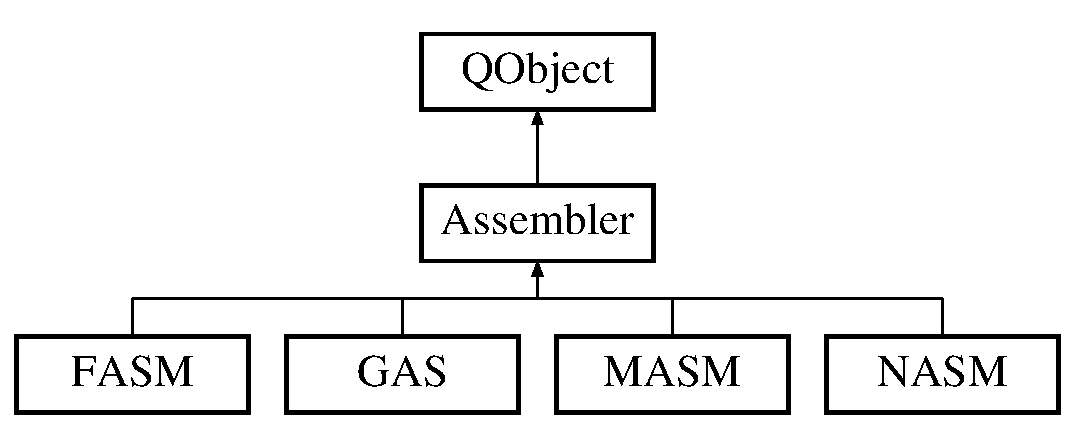
\includegraphics[height=3.000000cm]{class_assembler}
\end{center}
\end{figure}
\subsection*{Classes}
\begin{DoxyCompactItemize}
\item 
struct \hyperlink{struct_assembler_1_1_highlighting_rule}{Highlighting\+Rule}
\item 
struct \hyperlink{struct_assembler_1_1_line_num}{Line\+Num}
\end{DoxyCompactItemize}
\subsection*{Public Member Functions}
\begin{DoxyCompactItemize}
\item 
\hyperlink{class_assembler_aae6b7e0ee43e80cfbb0a0a130c1c476a}{Assembler} (bool x86, Q\+Object $\ast$parent=0)
\begin{DoxyCompactList}\small\item\em \hyperlink{class_assembler}{Assembler} constructor. Note that this is the stage where x86 is determined. \end{DoxyCompactList}\item 
\hypertarget{class_assembler_a0e5d1d3170d03c044a5d759267f31aa6}{}virtual Q\+String \hyperlink{class_assembler_a0e5d1d3170d03c044a5d759267f31aa6}{get\+Assembler\+Path} ()=0\label{class_assembler_a0e5d1d3170d03c044a5d759267f31aa6}

\begin{DoxyCompactList}\small\item\em Return the default path to the assembler. \end{DoxyCompactList}\item 
\hypertarget{class_assembler_a22e4678516dd765bc716915616b76ab9}{}virtual Q\+String \hyperlink{class_assembler_a22e4678516dd765bc716915616b76ab9}{get\+Linker\+Path} ()=0\label{class_assembler_a22e4678516dd765bc716915616b76ab9}

\begin{DoxyCompactList}\small\item\em Returns the default path to the linker. \end{DoxyCompactList}\item 
virtual quint64 \hyperlink{class_assembler_aa41f46e0cd774718d84bf4e5bd9c65b7}{get\+Main\+Offset} (Q\+File \&lst, Q\+String entry\+Label)=0
\item 
virtual void \hyperlink{class_assembler_aa724d277157a407d4d7fd3d0a23e84a7}{parse\+Lst\+File} (Q\+File \&lst, Q\+Vector$<$ \hyperlink{struct_assembler_1_1_line_num}{Assembler\+::\+Line\+Num} $>$ \&lines, quint64 offset)=0
\item 
\hypertarget{class_assembler_ace2439eeb3d887d279c3946df67f2525}{}virtual Q\+String \hyperlink{class_assembler_ace2439eeb3d887d279c3946df67f2525}{get\+Start\+Text} ()=0\label{class_assembler_ace2439eeb3d887d279c3946df67f2525}

\begin{DoxyCompactList}\small\item\em Return the default start text (default project code) \end{DoxyCompactList}\item 
\hypertarget{class_assembler_a3d699b729df36103f37a8ac45d54a0a6}{}virtual void \hyperlink{class_assembler_a3d699b729df36103f37a8ac45d54a0a6}{put\+Debug\+String} (\hyperlink{class_code_editor}{Code\+Editor} $\ast$code)=0\label{class_assembler_a3d699b729df36103f37a8ac45d54a0a6}

\begin{DoxyCompactList}\small\item\em Puts the debug string that makes frame (mov ebp, esp) \end{DoxyCompactList}\item 
\hypertarget{class_assembler_a7f4e8432d28694c2d89db13858ad1329}{}virtual Q\+String \hyperlink{class_assembler_a7f4e8432d28694c2d89db13858ad1329}{get\+Assembler\+Options} ()=0\label{class_assembler_a7f4e8432d28694c2d89db13858ad1329}

\begin{DoxyCompactList}\small\item\em Returns the default assembler options. \end{DoxyCompactList}\item 
\hypertarget{class_assembler_a644bcd38cf0b157d38c608043b63a6b8}{}virtual Q\+String \hyperlink{class_assembler_a644bcd38cf0b157d38c608043b63a6b8}{get\+Linker\+Options} ()=0\label{class_assembler_a644bcd38cf0b157d38c608043b63a6b8}

\begin{DoxyCompactList}\small\item\em Returns the default linker options. \end{DoxyCompactList}\item 
bool \hyperlink{class_assembler_aec6f08e8dd6ff49dfa9118be43ffc8e2}{isx86} ()
\begin{DoxyCompactList}\small\item\em Determines if the system is x86. \end{DoxyCompactList}\end{DoxyCompactItemize}
\subsection*{Public Attributes}
\begin{DoxyCompactItemize}
\item 
\hypertarget{class_assembler_a0a5d86a7ad035ed7113c4424c43d11fc}{}bool {\bfseries x86}\label{class_assembler_a0a5d86a7ad035ed7113c4424c43d11fc}

\item 
in C for example expressions for multi line highlighting workes if \hyperlink{class_assembler_a8e2ae531c6d59dfea8c7bb90febda262}{multi\+Line\+Comments}
\end{DoxyCompactItemize}


\subsection{Detailed Description}
This is the base class that all assemblers inherit. 

The \hyperlink{class_assembler}{Assembler} class contains functions which can be used to retrieve assember specific parameters such as the linker \& assembler location, the default program text, and user specified options. 

\subsection{Constructor \& Destructor Documentation}
\hypertarget{class_assembler_aae6b7e0ee43e80cfbb0a0a130c1c476a}{}\index{Assembler@{Assembler}!Assembler@{Assembler}}
\index{Assembler@{Assembler}!Assembler@{Assembler}}
\subsubsection[{Assembler}]{\setlength{\rightskip}{0pt plus 5cm}Assembler\+::\+Assembler (
\begin{DoxyParamCaption}
\item[{bool}]{x86, }
\item[{Q\+Object $\ast$}]{parent = {\ttfamily 0}}
\end{DoxyParamCaption}
)\hspace{0.3cm}{\ttfamily [explicit]}}\label{class_assembler_aae6b7e0ee43e80cfbb0a0a130c1c476a}


\hyperlink{class_assembler}{Assembler} constructor. Note that this is the stage where x86 is determined. 

Determines whether the target processor is x86 or x64. 

\subsection{Member Function Documentation}
\hypertarget{class_assembler_aa41f46e0cd774718d84bf4e5bd9c65b7}{}\index{Assembler@{Assembler}!get\+Main\+Offset@{get\+Main\+Offset}}
\index{get\+Main\+Offset@{get\+Main\+Offset}!Assembler@{Assembler}}
\subsubsection[{get\+Main\+Offset}]{\setlength{\rightskip}{0pt plus 5cm}virtual quint64 Assembler\+::get\+Main\+Offset (
\begin{DoxyParamCaption}
\item[{Q\+File \&}]{lst, }
\item[{Q\+String}]{entry\+Label}
\end{DoxyParamCaption}
)\hspace{0.3cm}{\ttfamily [pure virtual]}}\label{class_assembler_aa41f46e0cd774718d84bf4e5bd9c65b7}
get file with listing and name of entry label -\/ main or start. Returns the offset of this label -\/ number of strings and where the label is placed. 

Implemented in \hyperlink{class_f_a_s_m_ad63b8774910442ec8369db49a57cb7ee}{F\+A\+S\+M}, \hyperlink{class_m_a_s_m_aef0f1a5915184bfb9aca890a3493b3ad}{M\+A\+S\+M}, \hyperlink{class_g_a_s_ab1d4e22ffd3a438afa4dad4025ab2735}{G\+A\+S}, and \hyperlink{class_n_a_s_m_a432753e32490e7eaa36d9be41d8f1ed4}{N\+A\+S\+M}.

\hypertarget{class_assembler_aec6f08e8dd6ff49dfa9118be43ffc8e2}{}\index{Assembler@{Assembler}!isx86@{isx86}}
\index{isx86@{isx86}!Assembler@{Assembler}}
\subsubsection[{isx86}]{\setlength{\rightskip}{0pt plus 5cm}bool Assembler\+::isx86 (
\begin{DoxyParamCaption}
{}
\end{DoxyParamCaption}
)}\label{class_assembler_aec6f08e8dd6ff49dfa9118be43ffc8e2}


Determines if the system is x86. 

Returns a bool whether the processor is x86. \hypertarget{class_assembler_aa724d277157a407d4d7fd3d0a23e84a7}{}\index{Assembler@{Assembler}!parse\+Lst\+File@{parse\+Lst\+File}}
\index{parse\+Lst\+File@{parse\+Lst\+File}!Assembler@{Assembler}}
\subsubsection[{parse\+Lst\+File}]{\setlength{\rightskip}{0pt plus 5cm}virtual void Assembler\+::parse\+Lst\+File (
\begin{DoxyParamCaption}
\item[{Q\+File \&}]{lst, }
\item[{Q\+Vector$<$ {\bf Assembler\+::\+Line\+Num} $>$ \&}]{lines, }
\item[{quint64}]{offset}
\end{DoxyParamCaption}
)\hspace{0.3cm}{\ttfamily [pure virtual]}}\label{class_assembler_aa724d277157a407d4d7fd3d0a23e84a7}
Parses the listing file lst and fills Q\+Vector lines with results of parsing. offset -\/ difference between program code in memory and in file. 

Implemented in \hyperlink{class_f_a_s_m_aec5ded3222ad063755f28e113bf95e32}{F\+A\+S\+M}, \hyperlink{class_m_a_s_m_ad52eca298e722cee1e547f62ae24ee11}{M\+A\+S\+M}, \hyperlink{class_g_a_s_a572e0d7058f6f5d65a90c77a8b727460}{G\+A\+S}, and \hyperlink{class_n_a_s_m_a4de842373fdd8be68c23eb3313ad555e}{N\+A\+S\+M}.



\subsection{Member Data Documentation}
\hypertarget{class_assembler_a8e2ae531c6d59dfea8c7bb90febda262}{}\index{Assembler@{Assembler}!multi\+Line\+Comments@{multi\+Line\+Comments}}
\index{multi\+Line\+Comments@{multi\+Line\+Comments}!Assembler@{Assembler}}
\subsubsection[{multi\+Line\+Comments}]{\setlength{\rightskip}{0pt plus 5cm}in C for example expressions for multi line highlighting workes if Assembler\+::multi\+Line\+Comments}\label{class_assembler_a8e2ae531c6d59dfea8c7bb90febda262}
{\bfseries Initial value\+:}
\begin{DoxyCode}
== \textcolor{keyword}{true}. */
    \textcolor{keyword}{virtual} \textcolor{keywordtype}{void} fillHighligherRules(QVector<Assembler::HighlightingRule> &highlightingRules,
                                     QList<QTextCharFormat *> &formats,
                                     \textcolor{keywordtype}{bool} &\hyperlink{class_assembler_a8e2ae531c6d59dfea8c7bb90febda262}{multiLineComments},
                                     QRegExp &commentStartExpression,
                                     QRegExp &commentEndExpression) = 0
\end{DoxyCode}
Fills Q\+Vector with the highlighting rules. Qlist with formats (see \hyperlink{class_n_a_s_m}{N\+A\+S\+M}, \hyperlink{class_m_a_s_m}{M\+A\+S\+M}, \hyperlink{class_f_a_s_m}{F\+A\+S\+M}, \hyperlink{class_g_a_s}{G\+A\+S} as examples). comment\+Start\+Expression -\/ /$\ast$ in C++ for example, comment\+End\+Expression -\/ 

The documentation for this class was generated from the following files\+:\begin{DoxyCompactItemize}
\item 
\hyperlink{assembler_8h}{assembler.\+h}\item 
\hyperlink{assembler_8cpp}{assembler.\+cpp}\end{DoxyCompactItemize}

\hypertarget{class_code_editor}{}\section{Code\+Editor Class Reference}
\label{class_code_editor}\index{Code\+Editor@{Code\+Editor}}
Inheritance diagram for Code\+Editor\+:\begin{figure}[H]
\begin{center}
\leavevmode
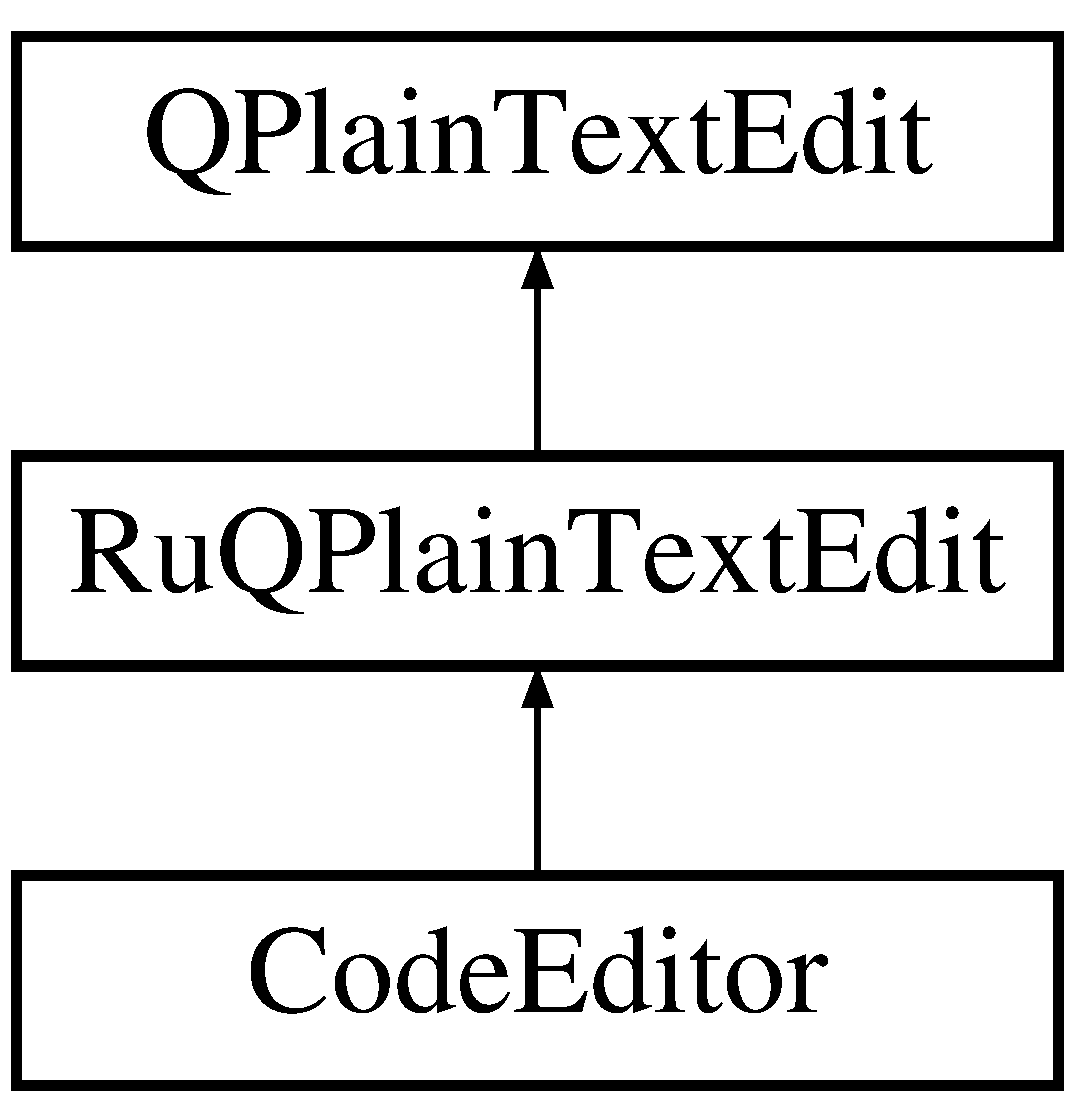
\includegraphics[height=3.000000cm]{class_code_editor}
\end{center}
\end{figure}
\subsection*{Public Slots}
\begin{DoxyCompactItemize}
\item 
\hypertarget{class_code_editor_ab460ede1cca49e5ba6e0d040efa2c00c}{}void {\bfseries update\+Debug\+Line} (int number)\label{class_code_editor_ab460ede1cca49e5ba6e0d040efa2c00c}

\item 
\hypertarget{class_code_editor_a93458bc38ed83c7501c1387a43252b1d}{}void {\bfseries put\+Tab} ()\label{class_code_editor_a93458bc38ed83c7501c1387a43252b1d}

\item 
\hypertarget{class_code_editor_a3bbced4ed50a16bb1ff830373a380464}{}void {\bfseries delete\+Tab} ()\label{class_code_editor_a3bbced4ed50a16bb1ff830373a380464}

\item 
\hypertarget{class_code_editor_a8d0bbb48f1f7ad273dba6e31f0b5f28b}{}void {\bfseries highlight\+Current\+Line} ()\label{class_code_editor_a8d0bbb48f1f7ad273dba6e31f0b5f28b}

\item 
\hypertarget{class_code_editor_aa38000763f508e8072ae87da7c56c8c7}{}void {\bfseries highlight\+Debug\+Line} (int line\+Number)\label{class_code_editor_aa38000763f508e8072ae87da7c56c8c7}

\item 
\hypertarget{class_code_editor_a020ee3dd5ffe336542199c4673846158}{}void {\bfseries set\+Debug\+Mode} (bool mode)\label{class_code_editor_a020ee3dd5ffe336542199c4673846158}

\item 
\hypertarget{class_code_editor_acf16c6a80c8403a2b51c1ac216d8dfef}{}Q\+List$<$ int $>$ $\ast$ {\bfseries get\+Breakpoints} ()\label{class_code_editor_acf16c6a80c8403a2b51c1ac216d8dfef}

\item 
\hypertarget{class_code_editor_ab9bd75edacef39851e1b6a2e149c2225}{}void {\bfseries set\+Breakpoint\+On\+Current\+Line} ()\label{class_code_editor_ab9bd75edacef39851e1b6a2e149c2225}

\end{DoxyCompactItemize}
\subsection*{Signals}
\begin{DoxyCompactItemize}
\item 
\hypertarget{class_code_editor_a462de76e30612853a2633b5175eaf778}{}void {\bfseries breakpoints\+Changed} (quint64 line\+Number, bool is\+Added)\label{class_code_editor_a462de76e30612853a2633b5175eaf778}

\item 
\hypertarget{class_code_editor_afb38d4c605648718eef7a15d8a1a4afd}{}void {\bfseries file\+Opened} (Q\+String path)\label{class_code_editor_afb38d4c605648718eef7a15d8a1a4afd}

\end{DoxyCompactItemize}
\subsection*{Public Member Functions}
\begin{DoxyCompactItemize}
\item 
\hypertarget{class_code_editor_a0f8a24cceec008bb6bd94c0dfc74aff5}{}{\bfseries Code\+Editor} (Q\+Widget $\ast$parent=0, bool with\+Beakpoints=true)\label{class_code_editor_a0f8a24cceec008bb6bd94c0dfc74aff5}

\item 
void \hyperlink{class_code_editor_a96e24088faa784a4ec419a647fcab5dd}{line\+Number\+Area\+Paint\+Event} (Q\+Paint\+Event $\ast$event)
\item 
void \hyperlink{class_code_editor_ae72a954985e8f12d755d22f33d6465ec}{line\+Number\+Area\+Mouse\+Press\+Event} (Q\+Mouse\+Event $\ast$event)
\item 
\hypertarget{class_code_editor_af7c3fbf0af03c4ff136e0298a336dd88}{}int {\bfseries line\+Number\+Area\+Width} ()\label{class_code_editor_af7c3fbf0af03c4ff136e0298a336dd88}

\item 
\hypertarget{class_code_editor_ab8e52f7d226ffbc0d7677e57ae138833}{}void {\bfseries repaint\+Line\+Number\+Area} ()\label{class_code_editor_ab8e52f7d226ffbc0d7677e57ae138833}

\item 
\hypertarget{class_code_editor_ad223a49b099ba8111fcd77a38b865166}{}bool {\bfseries is\+Macro\+On\+Current\+Debug\+Line} ()\label{class_code_editor_ad223a49b099ba8111fcd77a38b865166}

\end{DoxyCompactItemize}
\subsection*{Public Attributes}
\begin{DoxyCompactItemize}
\item 
\hypertarget{class_code_editor_a80d221047fe8770e4f44020d3dfdc211}{}int {\bfseries current\+Debug\+Line}\label{class_code_editor_a80d221047fe8770e4f44020d3dfdc211}

\item 
\hypertarget{class_code_editor_abfc08b4cdf3988f5325cb2bad954cc6a}{}bool {\bfseries debug\+Mode}\label{class_code_editor_abfc08b4cdf3988f5325cb2bad954cc6a}

\end{DoxyCompactItemize}
\subsection*{Protected Member Functions}
\begin{DoxyCompactItemize}
\item 
\hypertarget{class_code_editor_a3cf6c205d0cbcb3079811a406aab19be}{}void {\bfseries resize\+Event} (Q\+Resize\+Event $\ast$event)\label{class_code_editor_a3cf6c205d0cbcb3079811a406aab19be}

\item 
\hypertarget{class_code_editor_aa7addc3f760c1503bf8a2e57bb4b8678}{}void {\bfseries key\+Press\+Event} (Q\+Key\+Event $\ast$e)\label{class_code_editor_aa7addc3f760c1503bf8a2e57bb4b8678}

\item 
\hypertarget{class_code_editor_ae9ab9f58306591278621324da65bde40}{}void {\bfseries drag\+Enter\+Event} (Q\+Drag\+Enter\+Event $\ast$event)\label{class_code_editor_ae9ab9f58306591278621324da65bde40}

\item 
\hypertarget{class_code_editor_a4da88fc233cc1ff9cc96d08b7efd1033}{}void {\bfseries drop\+Event} (Q\+Drop\+Event $\ast$event)\label{class_code_editor_a4da88fc233cc1ff9cc96d08b7efd1033}

\end{DoxyCompactItemize}
\subsection*{Private Slots}
\begin{DoxyCompactItemize}
\item 
\hypertarget{class_code_editor_a28c8e8d686d9bacfb1bff04783b39924}{}void {\bfseries update\+Line\+Number\+Area\+Width} (int new\+Block\+Count)\label{class_code_editor_a28c8e8d686d9bacfb1bff04783b39924}

\item 
void \hyperlink{class_code_editor_a74597a5740a235410b56dfdd6f67314f}{update\+Line\+Number\+Area} (const Q\+Rect \&, int)
\item 
\hypertarget{class_code_editor_a0b95ac3b7c9fc3539f93b15fd3f3820e}{}void {\bfseries shift\+Breakpoints} (int block\+Count)\label{class_code_editor_a0b95ac3b7c9fc3539f93b15fd3f3820e}

\end{DoxyCompactItemize}
\subsection*{Private Attributes}
\begin{DoxyCompactItemize}
\item 
\hypertarget{class_code_editor_a9132cd18e435117ad928b18d9903162d}{}Q\+Widget $\ast$ {\bfseries line\+Number\+Area}\label{class_code_editor_a9132cd18e435117ad928b18d9903162d}

\item 
\hypertarget{class_code_editor_ab5e700e96549e80e5cc9023630ad2eff}{}int {\bfseries debug\+Area\+Width}\label{class_code_editor_ab5e700e96549e80e5cc9023630ad2eff}

\item 
\hypertarget{class_code_editor_aed60eae53d3dcaa0de4385c9204bd46e}{}Q\+Pixmap {\bfseries debug\+Image}\label{class_code_editor_aed60eae53d3dcaa0de4385c9204bd46e}

\item 
\hypertarget{class_code_editor_aadbfe61d58139da1b1a2d2f0afbcb078}{}Q\+Pixmap {\bfseries breakpoint\+Image}\label{class_code_editor_aadbfe61d58139da1b1a2d2f0afbcb078}

\item 
\hypertarget{class_code_editor_ae0315f118718e91bcc83188fd717e45d}{}Q\+List$<$ int $>$ \hyperlink{class_code_editor_ae0315f118718e91bcc83188fd717e45d}{breakpoints}\label{class_code_editor_ae0315f118718e91bcc83188fd717e45d}

\begin{DoxyCompactList}\small\item\em Number of lines with breakpoints. \end{DoxyCompactList}\item 
\hypertarget{class_code_editor_a77bda577cb6b2e1d83571ebbd22b86b1}{}int {\bfseries first\+Top\+Margin}\label{class_code_editor_a77bda577cb6b2e1d83571ebbd22b86b1}

\item 
\hypertarget{class_code_editor_a8465cd89547474011c78622dbfa76493}{}bool {\bfseries has\+Breakpoints}\label{class_code_editor_a8465cd89547474011c78622dbfa76493}

\item 
\hypertarget{class_code_editor_a9276c3f0db1928079d0a3cf990bb58cd}{}int {\bfseries prev\+Block\+Count}\label{class_code_editor_a9276c3f0db1928079d0a3cf990bb58cd}

\item 
\hypertarget{class_code_editor_af3744e9cba5fe24489514734fe0d37a1}{}Q\+Settings {\bfseries settings}\label{class_code_editor_af3744e9cba5fe24489514734fe0d37a1}

\end{DoxyCompactItemize}


\subsection{Member Function Documentation}
\hypertarget{class_code_editor_ae72a954985e8f12d755d22f33d6465ec}{}\index{Code\+Editor@{Code\+Editor}!line\+Number\+Area\+Mouse\+Press\+Event@{line\+Number\+Area\+Mouse\+Press\+Event}}
\index{line\+Number\+Area\+Mouse\+Press\+Event@{line\+Number\+Area\+Mouse\+Press\+Event}!Code\+Editor@{Code\+Editor}}
\subsubsection[{line\+Number\+Area\+Mouse\+Press\+Event}]{\setlength{\rightskip}{0pt plus 5cm}void Code\+Editor\+::line\+Number\+Area\+Mouse\+Press\+Event (
\begin{DoxyParamCaption}
\item[{Q\+Mouse\+Event $\ast$}]{event}
\end{DoxyParamCaption}
)}\label{class_code_editor_ae72a954985e8f12d755d22f33d6465ec}
If mouse click has been made -\/ add breakpoint Counting line number \hypertarget{class_code_editor_a96e24088faa784a4ec419a647fcab5dd}{}\index{Code\+Editor@{Code\+Editor}!line\+Number\+Area\+Paint\+Event@{line\+Number\+Area\+Paint\+Event}}
\index{line\+Number\+Area\+Paint\+Event@{line\+Number\+Area\+Paint\+Event}!Code\+Editor@{Code\+Editor}}
\subsubsection[{line\+Number\+Area\+Paint\+Event}]{\setlength{\rightskip}{0pt plus 5cm}void Code\+Editor\+::line\+Number\+Area\+Paint\+Event (
\begin{DoxyParamCaption}
\item[{Q\+Paint\+Event $\ast$}]{event}
\end{DoxyParamCaption}
)}\label{class_code_editor_a96e24088faa784a4ec419a647fcab5dd}
Blocks counting starts with 0, line number is equivalent (block number + 1) \hypertarget{class_code_editor_a74597a5740a235410b56dfdd6f67314f}{}\index{Code\+Editor@{Code\+Editor}!update\+Line\+Number\+Area@{update\+Line\+Number\+Area}}
\index{update\+Line\+Number\+Area@{update\+Line\+Number\+Area}!Code\+Editor@{Code\+Editor}}
\subsubsection[{update\+Line\+Number\+Area}]{\setlength{\rightskip}{0pt plus 5cm}void Code\+Editor\+::update\+Line\+Number\+Area (
\begin{DoxyParamCaption}
\item[{const Q\+Rect \&}]{rect, }
\item[{int}]{dy}
\end{DoxyParamCaption}
)\hspace{0.3cm}{\ttfamily [private]}, {\ttfamily [slot]}}\label{class_code_editor_a74597a5740a235410b56dfdd6f67314f}
Indirectly invokes \hyperlink{class_code_editor_a96e24088faa784a4ec419a647fcab5dd}{Code\+Editor\+::line\+Number\+Area\+Paint\+Event()} throw virtual Line\+Number\+Area\+::paint\+Event()

Viewport -\/ visible part of widget 

The documentation for this class was generated from the following files\+:\begin{DoxyCompactItemize}
\item 
\hyperlink{codeeditor_8h}{codeeditor.\+h}\item 
\hyperlink{codeeditor_8cpp}{codeeditor.\+cpp}\end{DoxyCompactItemize}

\hypertarget{class_command_debug_window}{}\section{Command\+Debug\+Window Class Reference}
\label{class_command_debug_window}\index{Command\+Debug\+Window@{Command\+Debug\+Window}}
Inheritance diagram for Command\+Debug\+Window\+:\begin{figure}[H]
\begin{center}
\leavevmode
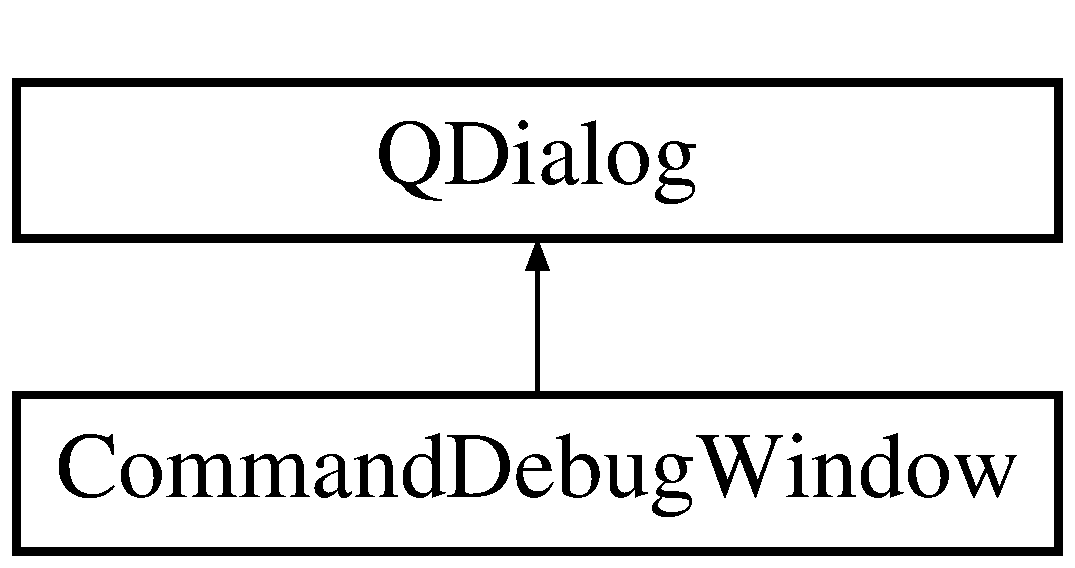
\includegraphics[height=2.000000cm]{class_command_debug_window}
\end{center}
\end{figure}
\subsection*{Public Slots}
\begin{DoxyCompactItemize}
\item 
\hypertarget{class_command_debug_window_abaaedef19fa6eb19aaf2ceeeb2ae4e99}{}void {\bfseries run\+Click} ()\label{class_command_debug_window_abaaedef19fa6eb19aaf2ceeeb2ae4e99}

\end{DoxyCompactItemize}
\subsection*{Signals}
\begin{DoxyCompactItemize}
\item 
\hypertarget{class_command_debug_window_aa6e7a92d27e60cd1c8c201310ff093e4}{}void {\bfseries run\+Command} (Q\+String command)\label{class_command_debug_window_aa6e7a92d27e60cd1c8c201310ff093e4}

\end{DoxyCompactItemize}
\subsection*{Public Member Functions}
\begin{DoxyCompactItemize}
\item 
\hypertarget{class_command_debug_window_aa9ea78c695bf4b4c0ff0314396282ccb}{}{\bfseries Command\+Debug\+Window} (Q\+Widget $\ast$parent=0)\label{class_command_debug_window_aa9ea78c695bf4b4c0ff0314396282ccb}

\end{DoxyCompactItemize}
\subsection*{Private Attributes}
\begin{DoxyCompactItemize}
\item 
\hypertarget{class_command_debug_window_a22110f0e3480da7ad1bff37e0824f4ca}{}Q\+H\+Box\+Layout $\ast$ {\bfseries add\+Layout}\label{class_command_debug_window_a22110f0e3480da7ad1bff37e0824f4ca}

\item 
\hypertarget{class_command_debug_window_a9f81804d9eafb39b9d68250e57da70d0}{}Q\+Push\+Button $\ast$ {\bfseries run\+Button}\label{class_command_debug_window_a9f81804d9eafb39b9d68250e57da70d0}

\item 
\hypertarget{class_command_debug_window_aaadd088f471e15d60bbbbd50b522c1ee}{}Q\+Line\+Edit $\ast$ {\bfseries command\+Name}\label{class_command_debug_window_aaadd088f471e15d60bbbbd50b522c1ee}

\end{DoxyCompactItemize}


The documentation for this class was generated from the following files\+:\begin{DoxyCompactItemize}
\item 
commanddebugwindow.\+h\item 
commanddebugwindow.\+cpp\end{DoxyCompactItemize}

\hypertarget{class_debug_any_command_widget}{}\section{Debug\+Any\+Command\+Widget Class Reference}
\label{class_debug_any_command_widget}\index{Debug\+Any\+Command\+Widget@{Debug\+Any\+Command\+Widget}}


This class does......  




{\ttfamily \#include $<$debuganycommandwidget.\+h$>$}

Inheritance diagram for Debug\+Any\+Command\+Widget\+:\begin{figure}[H]
\begin{center}
\leavevmode
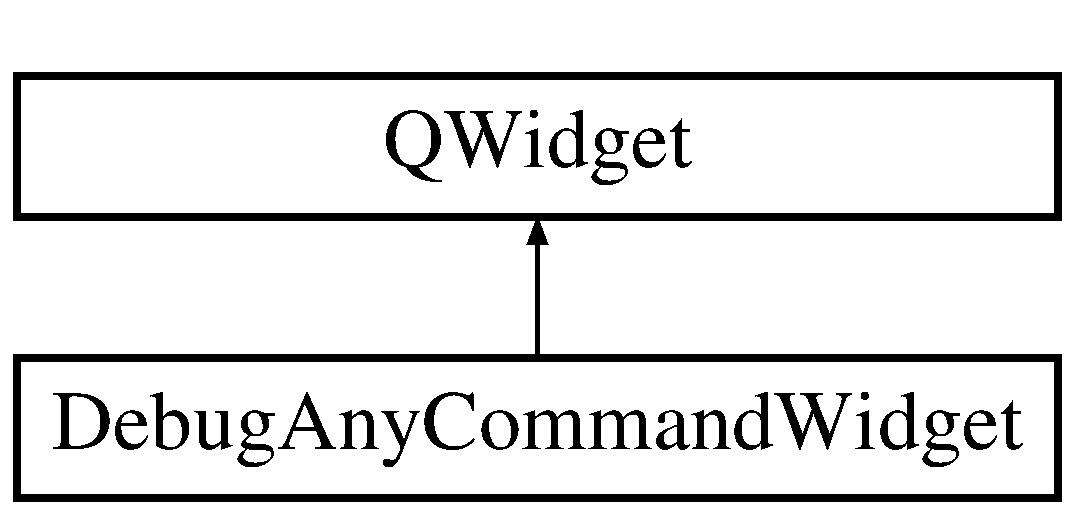
\includegraphics[height=2.000000cm]{class_debug_any_command_widget}
\end{center}
\end{figure}
\subsection*{Public Slots}
\begin{DoxyCompactItemize}
\item 
\hypertarget{class_debug_any_command_widget_a40f05f6e08e933dc99528e9f92195354}{}void {\bfseries process\+Command} ()\label{class_debug_any_command_widget_a40f05f6e08e933dc99528e9f92195354}

\end{DoxyCompactItemize}
\subsection*{Signals}
\begin{DoxyCompactItemize}
\item 
\hypertarget{class_debug_any_command_widget_a74bd41fd02dddc2455ce27f9fa75547c}{}void {\bfseries perform\+Command} (const Q\+String command, bool print)\label{class_debug_any_command_widget_a74bd41fd02dddc2455ce27f9fa75547c}

\end{DoxyCompactItemize}
\subsection*{Public Member Functions}
\begin{DoxyCompactItemize}
\item 
\hypertarget{class_debug_any_command_widget_ac518c5bebbf8b31eee1ea7863efea2fe}{}{\bfseries Debug\+Any\+Command\+Widget} (Q\+Widget $\ast$parent=0)\label{class_debug_any_command_widget_ac518c5bebbf8b31eee1ea7863efea2fe}

\item 
\hypertarget{class_debug_any_command_widget_a98dcf97a1ebf2a2a523dba4fa9553456}{}void {\bfseries set\+Focus\+On\+Line\+Edit} ()\label{class_debug_any_command_widget_a98dcf97a1ebf2a2a523dba4fa9553456}

\item 
\hypertarget{class_debug_any_command_widget_a0d5feefc9967dffc9ea4583fe909f815}{}void {\bfseries show\+Previous\+Command} ()\label{class_debug_any_command_widget_a0d5feefc9967dffc9ea4583fe909f815}

\item 
\hypertarget{class_debug_any_command_widget_aab67e1561b7532fb08ae3e60184e96b4}{}void {\bfseries show\+Next\+Command} ()\label{class_debug_any_command_widget_aab67e1561b7532fb08ae3e60184e96b4}

\item 
\hypertarget{class_debug_any_command_widget_aecb771425d29dfa3703c190bd2f027f2}{}int {\bfseries height} ()\label{class_debug_any_command_widget_aecb771425d29dfa3703c190bd2f027f2}

\end{DoxyCompactItemize}
\subsection*{Protected Member Functions}
\begin{DoxyCompactItemize}
\item 
\hypertarget{class_debug_any_command_widget_a14bbbbb6eb17d6f15bcc6ecd4e3e5aee}{}void {\bfseries key\+Press\+Event} (Q\+Key\+Event $\ast$event)\label{class_debug_any_command_widget_a14bbbbb6eb17d6f15bcc6ecd4e3e5aee}

\end{DoxyCompactItemize}
\subsection*{Private Attributes}
\begin{DoxyCompactItemize}
\item 
\hypertarget{class_debug_any_command_widget_ad4a5fe865ba9660f6cbac6e09e2bd137}{}Q\+Label $\ast$ {\bfseries any\+Command\+Label}\label{class_debug_any_command_widget_ad4a5fe865ba9660f6cbac6e09e2bd137}

\item 
\hypertarget{class_debug_any_command_widget_ad19beab3fb6c3792df1da5ec017da3e9}{}Q\+Line\+Edit $\ast$ {\bfseries command}\label{class_debug_any_command_widget_ad19beab3fb6c3792df1da5ec017da3e9}

\item 
\hypertarget{class_debug_any_command_widget_a50311daaf991957f859463ca1ea5cf9b}{}Q\+Push\+Button $\ast$ {\bfseries perform\+Button}\label{class_debug_any_command_widget_a50311daaf991957f859463ca1ea5cf9b}

\item 
\hypertarget{class_debug_any_command_widget_a6dd7d633f09779a465218436d9bac391}{}Q\+H\+Box\+Layout $\ast$ {\bfseries layout}\label{class_debug_any_command_widget_a6dd7d633f09779a465218436d9bac391}

\item 
\hypertarget{class_debug_any_command_widget_a24fa59fe04b41dcdb695bb6aae7d94a1}{}Q\+Check\+Box $\ast$ {\bfseries print\+Check\+Box}\label{class_debug_any_command_widget_a24fa59fe04b41dcdb695bb6aae7d94a1}

\item 
\hypertarget{class_debug_any_command_widget_aa6e9673465d405354506a286f6e54075}{}Q\+String\+List {\bfseries commands}\label{class_debug_any_command_widget_aa6e9673465d405354506a286f6e54075}

\item 
\hypertarget{class_debug_any_command_widget_a1ba9dd8b19df99e7ae62598f31bcc6f9}{}int {\bfseries current\+Command\+Pos}\label{class_debug_any_command_widget_a1ba9dd8b19df99e7ae62598f31bcc6f9}

\end{DoxyCompactItemize}


\subsection{Detailed Description}
This class does...... 



The documentation for this class was generated from the following files\+:\begin{DoxyCompactItemize}
\item 
\hyperlink{debuganycommandwidget_8h}{debuganycommandwidget.\+h}\item 
\hyperlink{debuganycommandwidget_8cpp}{debuganycommandwidget.\+cpp}\end{DoxyCompactItemize}

\hypertarget{class_debugger}{}\section{Debugger Class Reference}
\label{class_debugger}\index{Debugger@{Debugger}}


This class represents the debugger.  




{\ttfamily \#include $<$debugger.\+h$>$}

Inheritance diagram for Debugger\+:\begin{figure}[H]
\begin{center}
\leavevmode
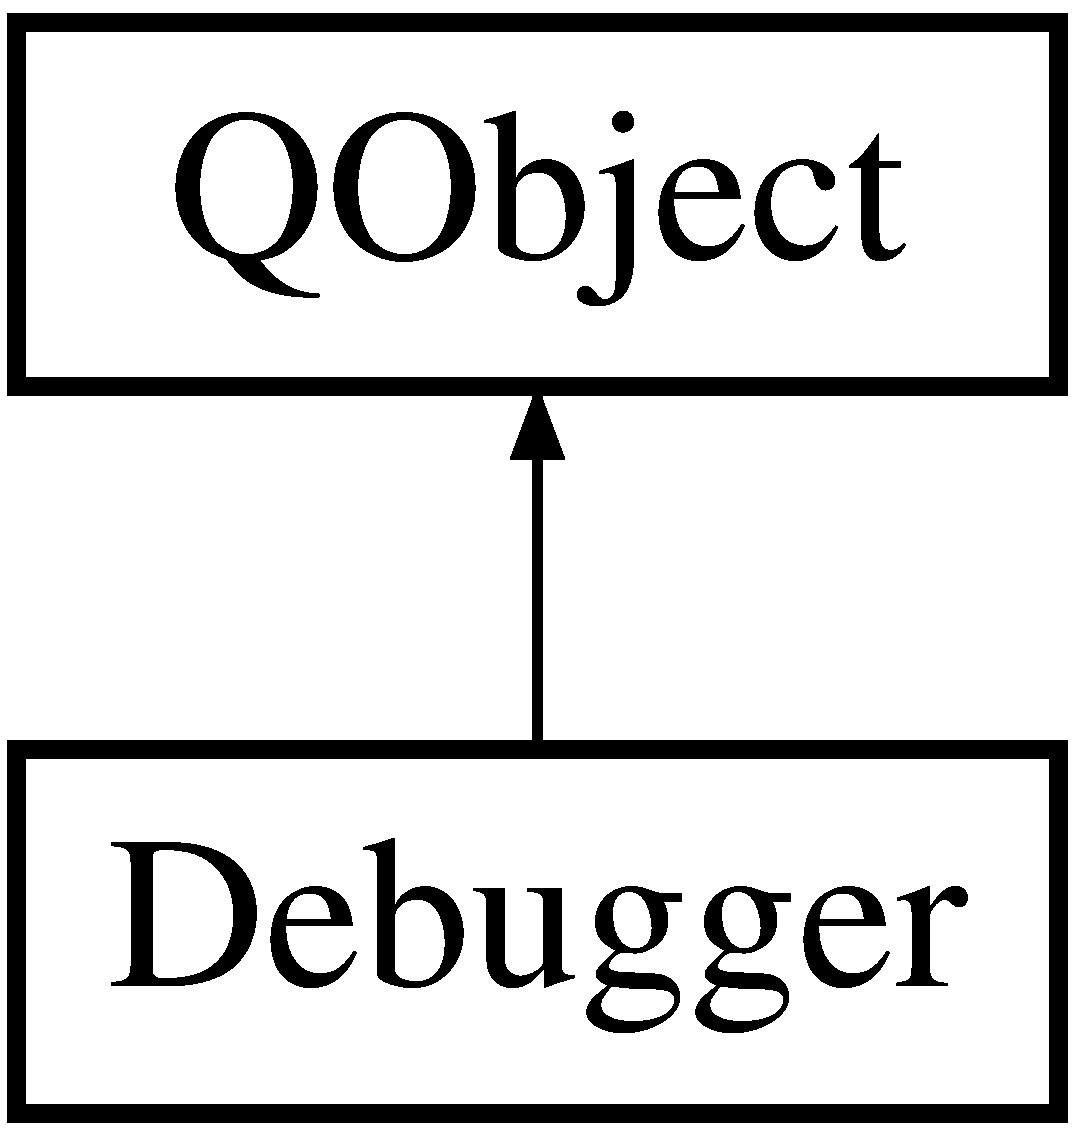
\includegraphics[height=2.000000cm]{class_debugger}
\end{center}
\end{figure}
\subsection*{Classes}
\begin{DoxyCompactItemize}
\item 
struct \hyperlink{struct_debugger_1_1memory_info}{memory\+Info}
\item 
struct \hyperlink{struct_debugger_1_1registers_info}{registers\+Info}
\end{DoxyCompactItemize}
\subsection*{Public Types}
\begin{DoxyCompactItemize}
\item 
\hypertarget{class_debugger_a80544446d8b2aebeb64fc2dd21ce189f}{}typedef \hyperlink{struct_assembler_1_1_line_num}{Assembler\+::\+Line\+Num} {\bfseries Line\+Num}\label{class_debugger_a80544446d8b2aebeb64fc2dd21ce189f}

\end{DoxyCompactItemize}
\subsection*{Public Slots}
\begin{DoxyCompactItemize}
\item 
\hypertarget{class_debugger_ac89ff4b6cda77d27cf45eaec8d06eb84}{}void {\bfseries read\+Output\+To\+Buffer} ()\label{class_debugger_ac89ff4b6cda77d27cf45eaec8d06eb84}

\item 
\hypertarget{class_debugger_ae0be5fc23e7513a9b943b02b8464655c}{}void {\bfseries process\+Output} ()\label{class_debugger_ae0be5fc23e7513a9b943b02b8464655c}

\item 
\hypertarget{class_debugger_af4417fa18d936f6f9275c85e9ded4705}{}void {\bfseries process\+Message} (Q\+String output, Q\+String error)\label{class_debugger_af4417fa18d936f6f9275c85e9ded4705}

\item 
\hypertarget{class_debugger_ae53701dbcf8dbc4378b0fc3769a988f0}{}void {\bfseries process\+Action} (Q\+String output, Q\+String error=Q\+String())\label{class_debugger_ae53701dbcf8dbc4378b0fc3769a988f0}

\item 
\hypertarget{class_debugger_a6f3eae0ace3af6bf40be6cd69ca98f22}{}void {\bfseries do\+Input} (Q\+String command, Debug\+Action\+Type action\+Type)\label{class_debugger_a6f3eae0ace3af6bf40be6cd69ca98f22}

\item 
\hypertarget{class_debugger_ac18e41fff794085b939abb643d5547ae}{}void {\bfseries change\+Breakpoint} (quint64 line\+Number, bool is\+Added)\label{class_debugger_ac18e41fff794085b939abb643d5547ae}

\item 
\hypertarget{class_debugger_a83af2b195bc1dd89cb05121585ba97bf}{}void {\bfseries emit\+Started} ()\label{class_debugger_a83af2b195bc1dd89cb05121585ba97bf}

\end{DoxyCompactItemize}
\subsection*{Signals}
\begin{DoxyCompactItemize}
\item 
\hypertarget{class_debugger_adbe43a9b006c1ff0df00f959022a180c}{}void \hyperlink{class_debugger_adbe43a9b006c1ff0df00f959022a180c}{highlight\+Line} (int)\label{class_debugger_adbe43a9b006c1ff0df00f959022a180c}

\begin{DoxyCompactList}\small\item\em Highlight the current debug line. \end{DoxyCompactList}\item 
\hypertarget{class_debugger_acf0d732e2bd6411e03c3e3f7ab072db4}{}void {\bfseries finished} ()\label{class_debugger_acf0d732e2bd6411e03c3e3f7ab072db4}

\item 
\hypertarget{class_debugger_ae3c0d16ffb07fca28532471dac4a3d04}{}void \hyperlink{class_debugger_ae3c0d16ffb07fca28532471dac4a3d04}{started} ()\label{class_debugger_ae3c0d16ffb07fca28532471dac4a3d04}

\begin{DoxyCompactList}\small\item\em Emited when debugger is ready to get commands like step into, etc. -\/$>$ Omitted or Emited? \end{DoxyCompactList}\item 
\hypertarget{class_debugger_a97bb6cfc618c4f76d09c245def0cc6fe}{}void {\bfseries print\+Registers} (Q\+List$<$ \hyperlink{struct_debugger_1_1registers_info}{Debugger\+::registers\+Info} $>$)\label{class_debugger_a97bb6cfc618c4f76d09c245def0cc6fe}

\item 
\hypertarget{class_debugger_ac17eb18b4f55846b2ee26d20081165d6}{}void {\bfseries print\+Memory} (Q\+List$<$ \hyperlink{struct_debugger_1_1memory_info}{Debugger\+::memory\+Info} $>$)\label{class_debugger_ac17eb18b4f55846b2ee26d20081165d6}

\item 
\hypertarget{class_debugger_aaa170ace8d83be4d6d50eb77452b9970}{}void {\bfseries print\+Log} (Q\+String msg, Q\+Color color=Q\+Color(Qt\+::black))\label{class_debugger_aaa170ace8d83be4d6d50eb77452b9970}

\item 
\hypertarget{class_debugger_a33c5be2b419f3917f460eac35d5472b0}{}void {\bfseries print\+Output} (Q\+String msg)\label{class_debugger_a33c5be2b419f3917f460eac35d5472b0}

\item 
\hypertarget{class_debugger_a7652cfcdc33f9c8d5ea82bcf1d2f497d}{}void {\bfseries in\+Macro} ()\label{class_debugger_a7652cfcdc33f9c8d5ea82bcf1d2f497d}

\item 
\hypertarget{class_debugger_ac31d9a6bd5f7096346fc1e0d693556dd}{}void {\bfseries was\+Stopped} ()\label{class_debugger_ac31d9a6bd5f7096346fc1e0d693556dd}

\item 
\hypertarget{class_debugger_a2d80e136e4642751be887681efcc0ad5}{}void {\bfseries need\+To\+Continue} ()\label{class_debugger_a2d80e136e4642751be887681efcc0ad5}

\end{DoxyCompactItemize}
\subsection*{Public Member Functions}
\begin{DoxyCompactItemize}
\item 
\hypertarget{class_debugger_afbf5c91cfe0f4bf6953bd241af0b6b0a}{}{\bfseries Debugger} (Q\+Text\+Edit $\ast$t\+Edit, const Q\+String \&path, Q\+String tmp, \hyperlink{class_assembler}{Assembler} $\ast$assembler, Q\+Widget $\ast$parent=0)\label{class_debugger_afbf5c91cfe0f4bf6953bd241af0b6b0a}

\item 
\hypertarget{class_debugger_afcddd18a500da8763d72a0714486956a}{}void {\bfseries set\+Watches\+Count} (int count)\label{class_debugger_afcddd18a500da8763d72a0714486956a}

\item 
\hypertarget{class_debugger_a0d42b6de1ebec7605bcf3b6cab2eb65d}{}bool {\bfseries is\+Stopped} ()\label{class_debugger_a0d42b6de1ebec7605bcf3b6cab2eb65d}

\item 
\hypertarget{class_debugger_a6f041e29ae97defbde7ed711fb175e62}{}void {\bfseries pause} ()\label{class_debugger_a6f041e29ae97defbde7ed711fb175e62}

\end{DoxyCompactItemize}
\subsection*{Private Member Functions}
\begin{DoxyCompactItemize}
\item 
\hypertarget{class_debugger_a5e5bd24a61e98d7854ff9f1b5a79cd1e}{}void {\bfseries process\+Lst} ()\label{class_debugger_a5e5bd24a61e98d7854ff9f1b5a79cd1e}

\item 
\hypertarget{class_debugger_a1df28a43e7686d9aa06714fc8b534072}{}void {\bfseries run} ()\label{class_debugger_a1df28a43e7686d9aa06714fc8b534072}

\end{DoxyCompactItemize}
\subsection*{Private Attributes}
\begin{DoxyCompactItemize}
\item 
\hypertarget{class_debugger_a3d2a0063b413ae6b22a1c970d6fa255c}{}Q\+Process $\ast$ {\bfseries process}\label{class_debugger_a3d2a0063b413ae6b22a1c970d6fa255c}

\item 
\hypertarget{class_debugger_a99e176dedc29ecb4a7995df3c853c43c}{}Q\+Text\+Edit $\ast$ {\bfseries text\+Edit}\label{class_debugger_a99e176dedc29ecb4a7995df3c853c43c}

\item 
\hypertarget{class_debugger_a9520cdbe94f115c987328c526116323b}{}quint64 \hyperlink{class_debugger_a9520cdbe94f115c987328c526116323b}{offset}\label{class_debugger_a9520cdbe94f115c987328c526116323b}

\begin{DoxyCompactList}\small\item\em Offset between program code in memory and in file. \end{DoxyCompactList}\item 
\hypertarget{class_debugger_acf8d80ba5fb7408aef12c82b687ae416}{}Q\+Vector$<$ \hyperlink{struct_assembler_1_1_line_num}{Line\+Num} $>$ \hyperlink{class_debugger_acf8d80ba5fb7408aef12c82b687ae416}{lines}\label{class_debugger_acf8d80ba5fb7408aef12c82b687ae416}

\begin{DoxyCompactList}\small\item\em Accordance between program lines in memory and in file. \end{DoxyCompactList}\item 
\hypertarget{class_debugger_a685a71e032e775b881e76fb62b9bf702}{}int \hyperlink{class_debugger_a685a71e032e775b881e76fb62b9bf702}{c}\label{class_debugger_a685a71e032e775b881e76fb62b9bf702}

\begin{DoxyCompactList}\small\item\em Counter for sequential performing of actions. \end{DoxyCompactList}\item 
\hypertarget{class_debugger_a2868873b7e2c82002aca656a4c88d1d1}{}bool {\bfseries registers\+Ok}\label{class_debugger_a2868873b7e2c82002aca656a4c88d1d1}

\item 
\hypertarget{class_debugger_a3d7e051e61a7d69df940301617860640}{}Q\+Queue$<$ Debug\+Action\+Type $>$ \hyperlink{class_debugger_a3d7e051e61a7d69df940301617860640}{action\+Type\+Queue}\label{class_debugger_a3d7e051e61a7d69df940301617860640}

\begin{DoxyCompactList}\small\item\em Queue of actions type from enum. \end{DoxyCompactList}\item 
\hypertarget{class_debugger_a20e69b676082292edf0fdbee0a13aeb0}{}Q\+String \hyperlink{class_debugger_a20e69b676082292edf0fdbee0a13aeb0}{exit\+Message}\label{class_debugger_a20e69b676082292edf0fdbee0a13aeb0}

\begin{DoxyCompactList}\small\item\em Message on exit in current platform. \end{DoxyCompactList}\item 
\hypertarget{class_debugger_af5894be0b78a8cc36b1d1b99dd71ef97}{}Q\+Reg\+Exp \hyperlink{class_debugger_af5894be0b78a8cc36b1d1b99dd71ef97}{c\+Exit\+Message}\label{class_debugger_af5894be0b78a8cc36b1d1b99dd71ef97}

\begin{DoxyCompactList}\small\item\em Message on exit which shows when \char`\"{}continue\char`\"{} command used. \end{DoxyCompactList}\item 
\hypertarget{class_debugger_a9182a784eaf8f0e5fd6fd56c4d78000a}{}Q\+String {\bfseries tmp\+Path}\label{class_debugger_a9182a784eaf8f0e5fd6fd56c4d78000a}

\item 
\hypertarget{class_debugger_a55d82d638b0be2683dcf654696e994c0}{}Q\+String \hyperlink{class_debugger_a55d82d638b0be2683dcf654696e994c0}{buffer}\label{class_debugger_a55d82d638b0be2683dcf654696e994c0}

\begin{DoxyCompactList}\small\item\em Global gdb output buffer. \end{DoxyCompactList}\item 
\hypertarget{class_debugger_aa81988662cf102a4b9db3f5e05b4da1c}{}Q\+String \hyperlink{class_debugger_aa81988662cf102a4b9db3f5e05b4da1c}{error\+Buffer}\label{class_debugger_aa81988662cf102a4b9db3f5e05b4da1c}

\begin{DoxyCompactList}\small\item\em Global gdb error buffer. \end{DoxyCompactList}\item 
\hypertarget{class_debugger_a991fd6cbd4a6b6983f1c4913600df67f}{}Q\+Timer $\ast$ \hyperlink{class_debugger_a991fd6cbd4a6b6983f1c4913600df67f}{buffer\+Timer}\label{class_debugger_a991fd6cbd4a6b6983f1c4913600df67f}

\begin{DoxyCompactList}\small\item\em Timer for checking output and sending ready output to processing with Debugger\+::process\+Output() function. \end{DoxyCompactList}\item 
\hypertarget{class_debugger_a3a9f51bd7e9885d57408177656ef9903}{}int \hyperlink{class_debugger_a3a9f51bd7e9885d57408177656ef9903}{watches\+Count}\label{class_debugger_a3a9f51bd7e9885d57408177656ef9903}

\begin{DoxyCompactList}\small\item\em The number of variable watches. \end{DoxyCompactList}\item 
\hypertarget{class_debugger_ae8d68c1ebbcd62fbadb3d4f494eac132}{}Q\+List$<$ \hyperlink{struct_debugger_1_1memory_info}{Debugger\+::memory\+Info} $>$ \hyperlink{class_debugger_ae8d68c1ebbcd62fbadb3d4f494eac132}{watches}\label{class_debugger_ae8d68c1ebbcd62fbadb3d4f494eac132}

\begin{DoxyCompactList}\small\item\em List of the variable watches. \end{DoxyCompactList}\item 
\hypertarget{class_debugger_a034fcdc2cfeac7d404eaf22f3cec72b9}{}bool \hyperlink{class_debugger_a034fcdc2cfeac7d404eaf22f3cec72b9}{first\+Action}\label{class_debugger_a034fcdc2cfeac7d404eaf22f3cec72b9}

\begin{DoxyCompactList}\small\item\em U\+N\+K\+N\+O\+W\+N. \end{DoxyCompactList}\item 
\hypertarget{class_debugger_a653485bb08b57e6505c2f98fee8df379}{}Q\+List$<$ \hyperlink{struct_assembler_1_1_line_num}{Line\+Num} $>$ \hyperlink{class_debugger_a653485bb08b57e6505c2f98fee8df379}{break\+Pairs}\label{class_debugger_a653485bb08b57e6505c2f98fee8df379}

\begin{DoxyCompactList}\small\item\em U\+N\+K\+N\+O\+W\+N. \end{DoxyCompactList}\item 
\hypertarget{class_debugger_a820589c5102d67769128d41a17754d07}{}\hyperlink{class_assembler}{Assembler} $\ast$ {\bfseries assembler}\label{class_debugger_a820589c5102d67769128d41a17754d07}

\item 
\hypertarget{class_debugger_a97f6c18d3d76887b7cb4dbb15aa8d44d}{}bool {\bfseries stopped}\label{class_debugger_a97f6c18d3d76887b7cb4dbb15aa8d44d}

\item 
\hypertarget{class_debugger_af48358ff43c602ca6cf1766c0ebff92a}{}quint64 {\bfseries pid}\label{class_debugger_af48358ff43c602ca6cf1766c0ebff92a}

\item 
\hypertarget{class_debugger_a407fb1b514f65eae94dede657442a327}{}bool {\bfseries dbg\+Symbols}\label{class_debugger_a407fb1b514f65eae94dede657442a327}

\item 
\hypertarget{class_debugger_a8f11bcbf15b0d90b62f0d44bdfe2e404}{}quint64 {\bfseries entry\+Point}\label{class_debugger_a8f11bcbf15b0d90b62f0d44bdfe2e404}

\end{DoxyCompactItemize}


\subsection{Detailed Description}
This class represents the debugger. 

! 

The documentation for this class was generated from the following files\+:\begin{DoxyCompactItemize}
\item 
\hyperlink{debugger_8h}{debugger.\+h}\item 
\hyperlink{debugger_8cpp}{debugger.\+cpp}\end{DoxyCompactItemize}

\hypertarget{class_debug_table_widget}{}\section{Debug\+Table\+Widget Class Reference}
\label{class_debug_table_widget}\index{Debug\+Table\+Widget@{Debug\+Table\+Widget}}


This class represents the Memory table.  




{\ttfamily \#include $<$debugtablewidget.\+h$>$}

Inheritance diagram for Debug\+Table\+Widget\+:\begin{figure}[H]
\begin{center}
\leavevmode
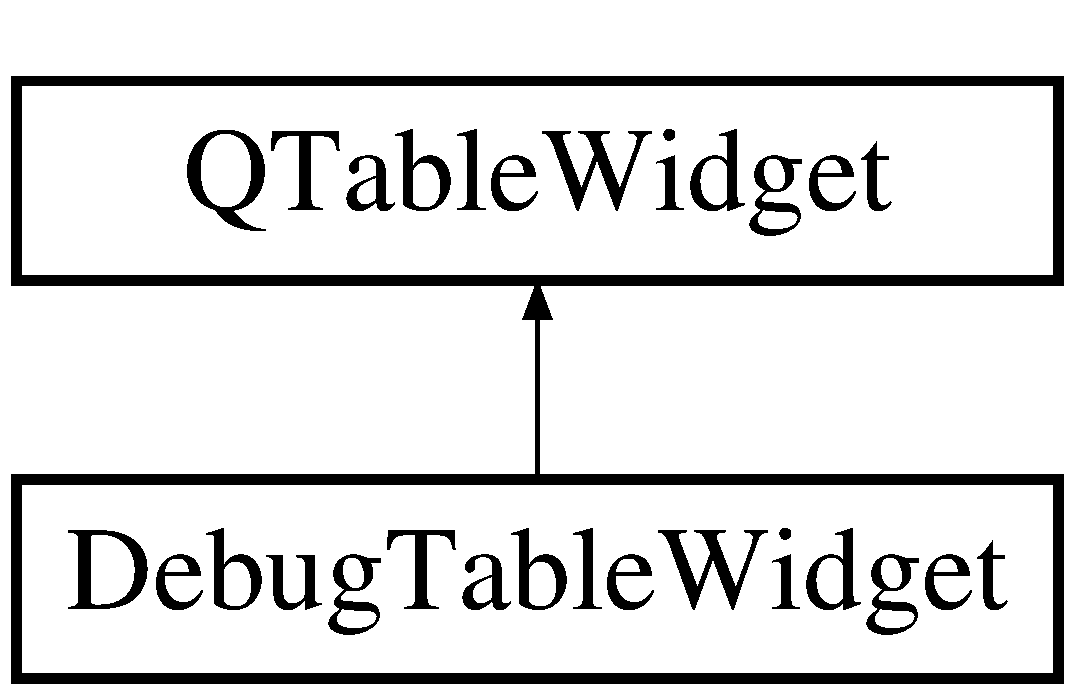
\includegraphics[height=2.000000cm]{class_debug_table_widget}
\end{center}
\end{figure}
\subsection*{Public Slots}
\begin{DoxyCompactItemize}
\item 
\hypertarget{class_debug_table_widget_a4d8800af67dcf41b00c9c99f7cf136dc}{}void {\bfseries delete\+Variable} ()\label{class_debug_table_widget_a4d8800af67dcf41b00c9c99f7cf136dc}

\item 
\hypertarget{class_debug_table_widget_a643c2921c5092af91a16bfea6246e96d}{}void {\bfseries add\+Variable} (const Q\+String \&variable\+Name, int row\+Number=-\/1)\label{class_debug_table_widget_a643c2921c5092af91a16bfea6246e96d}

\item 
\hypertarget{class_debug_table_widget_a09c0ea8ad8301fb33343855b8a1ceaea}{}void {\bfseries add\+Variable} (const \hyperlink{struct_ru_q_plain_text_edit_1_1_watch}{Ru\+Q\+Plain\+Text\+Edit\+::\+Watch} \&variable, int row\+Number=-\/1)\label{class_debug_table_widget_a09c0ea8ad8301fb33343855b8a1ceaea}

\item 
\hypertarget{class_debug_table_widget_a655c0e61ba8232d0ae3a06c5b83c8ab9}{}void {\bfseries change\+Variable\+Value} (const Q\+String \&value, int row\+Number, bool is\+Valid)\label{class_debug_table_widget_a655c0e61ba8232d0ae3a06c5b83c8ab9}

\item 
\hypertarget{class_debug_table_widget_a26bcee1edac0ec77e94a158bf460fdc0}{}void {\bfseries add\+Register} (const Q\+String \&name, const Q\+String \&hex\+Value, const Q\+String \&dec\+Value, int row\+Number)\label{class_debug_table_widget_a26bcee1edac0ec77e94a158bf460fdc0}

\item 
\hypertarget{class_debug_table_widget_a5ef2ed2a7b735973df658db91ca37fd2}{}void {\bfseries change\+Memory\+Window} (int row, int column)\label{class_debug_table_widget_a5ef2ed2a7b735973df658db91ca37fd2}

\item 
\hypertarget{class_debug_table_widget_acb9c92b66e566a16bb71fb68fb39cf5c}{}void {\bfseries set\+Values\+From\+Debugger} (Q\+List$<$ \hyperlink{struct_debugger_1_1memory_info}{Debugger\+::memory\+Info} $>$ watches)\label{class_debug_table_widget_acb9c92b66e566a16bb71fb68fb39cf5c}

\item 
\hypertarget{class_debug_table_widget_ab2631afd9b17c3f5246fad297b02c0b7}{}void {\bfseries set\+Values\+From\+Debugger} (Q\+List$<$ \hyperlink{struct_debugger_1_1registers_info}{Debugger\+::registers\+Info} $>$ registers)\label{class_debug_table_widget_ab2631afd9b17c3f5246fad297b02c0b7}

\end{DoxyCompactItemize}
\subsection*{Signals}
\begin{DoxyCompactItemize}
\item 
\hypertarget{class_debug_table_widget_a63febd4042d44b0148fb3e3692d4423b}{}void {\bfseries close\+Signal} ()\label{class_debug_table_widget_a63febd4042d44b0148fb3e3692d4423b}

\item 
\hypertarget{class_debug_table_widget_a4ba5bb4bf0bc8ffac4fa7740cc566dc4}{}void {\bfseries debug\+Show\+Memory} ()\label{class_debug_table_widget_a4ba5bb4bf0bc8ffac4fa7740cc566dc4}

\end{DoxyCompactItemize}
\subsection*{Public Member Functions}
\begin{DoxyCompactItemize}
\item 
\hypertarget{class_debug_table_widget_a72e7b44f66614eb549fe23486c885c57}{}{\bfseries Debug\+Table\+Widget} (int rows, int columns, Debug\+Table\+Widget\+Type widget\+Type, Q\+Widget $\ast$parent=0)\label{class_debug_table_widget_a72e7b44f66614eb549fe23486c885c57}

\item 
\hypertarget{class_debug_table_widget_a9242e8c7c39e7cc52f1689dfabd69285}{}bool {\bfseries is\+Empty} ()\label{class_debug_table_widget_a9242e8c7c39e7cc52f1689dfabd69285}

\item 
\hypertarget{class_debug_table_widget_a4b3a88d8c20725d4515af9222805f7af}{}void {\bfseries initialize\+Memory\+Window} (const Q\+List$<$ \hyperlink{struct_ru_q_plain_text_edit_1_1_watch}{Ru\+Q\+Plain\+Text\+Edit\+::\+Watch} $>$ \&watches)\label{class_debug_table_widget_a4b3a88d8c20725d4515af9222805f7af}

\end{DoxyCompactItemize}
\subsection*{Static Public Attributes}
\begin{DoxyCompactItemize}
\item 
\hypertarget{class_debug_table_widget_a0ed3f2adc6845b3577c4395e64839252}{}static Q\+Byte\+Array {\bfseries memory\+Header\+State}\label{class_debug_table_widget_a0ed3f2adc6845b3577c4395e64839252}

\item 
\hypertarget{class_debug_table_widget_a91db0ae3cf15652b8df4284c2714b4da}{}static Q\+Byte\+Array {\bfseries register\+Window\+State}\label{class_debug_table_widget_a91db0ae3cf15652b8df4284c2714b4da}

\item 
\hypertarget{class_debug_table_widget_ad78dd6c6a348da08ad18dfdbf6272c77}{}static bool {\bfseries geometry\+Memory\+Saved}\label{class_debug_table_widget_ad78dd6c6a348da08ad18dfdbf6272c77}

\item 
\hypertarget{class_debug_table_widget_a0b98bcbe0af39cad3262901a24e72f1b}{}static bool {\bfseries geometry\+Registers\+Saved}\label{class_debug_table_widget_a0b98bcbe0af39cad3262901a24e72f1b}

\end{DoxyCompactItemize}
\subsection*{Protected Member Functions}
\begin{DoxyCompactItemize}
\item 
\hypertarget{class_debug_table_widget_a1f54a1476d5e6b593a7122f125302791}{}void {\bfseries close\+Event} (Q\+Close\+Event $\ast$)\label{class_debug_table_widget_a1f54a1476d5e6b593a7122f125302791}

\item 
\hypertarget{class_debug_table_widget_a9916b91e7858973c3611ddeba648c69a}{}void {\bfseries mouse\+Press\+Event} (Q\+Mouse\+Event $\ast$event)\label{class_debug_table_widget_a9916b91e7858973c3611ddeba648c69a}

\item 
\hypertarget{class_debug_table_widget_ae2d309bb3c50be05fbc715d67522de66}{}void {\bfseries key\+Press\+Event} (Q\+Key\+Event $\ast$event)\label{class_debug_table_widget_ae2d309bb3c50be05fbc715d67522de66}

\end{DoxyCompactItemize}
\subsection*{Private Attributes}
\begin{DoxyCompactItemize}
\item 
\hypertarget{class_debug_table_widget_aeed4234d2e5094f6af154e0a65916f71}{}int {\bfseries context\+Menu\+Line\+Number}\label{class_debug_table_widget_aeed4234d2e5094f6af154e0a65916f71}

\item 
\hypertarget{class_debug_table_widget_acb026ff25f4f9cd6023701b0364abeac}{}Debug\+Table\+Widget\+Type {\bfseries type}\label{class_debug_table_widget_acb026ff25f4f9cd6023701b0364abeac}

\item 
\hypertarget{class_debug_table_widget_a0257a292e3dd8583b6e9294a7df1b7c0}{}bool {\bfseries empty}\label{class_debug_table_widget_a0257a292e3dd8583b6e9294a7df1b7c0}

\item 
\hypertarget{class_debug_table_widget_a1221dfd2571c4ae8c344a3d71a4953e4}{}bool {\bfseries first\+Time}\label{class_debug_table_widget_a1221dfd2571c4ae8c344a3d71a4953e4}

\end{DoxyCompactItemize}


\subsection{Detailed Description}
This class represents the Memory table. 

!\+This class contains the methods and variables relevant to the memory window under the debugger. Methods include adding variable watches, modifying variable contents, and adding registers. 

The documentation for this class was generated from the following files\+:\begin{DoxyCompactItemize}
\item 
\hyperlink{debugtablewidget_8h}{debugtablewidget.\+h}\item 
\hyperlink{debugtablewidget_8cpp}{debugtablewidget.\+cpp}\end{DoxyCompactItemize}

\hypertarget{class_f_a_s_m}{}\section{F\+A\+S\+M Class Reference}
\label{class_f_a_s_m}\index{F\+A\+S\+M@{F\+A\+S\+M}}


This class defines the behavior for the \hyperlink{class_f_a_s_m}{F\+A\+S\+M} assembler.  




{\ttfamily \#include $<$fasm.\+h$>$}

Inheritance diagram for F\+A\+S\+M\+:\begin{figure}[H]
\begin{center}
\leavevmode
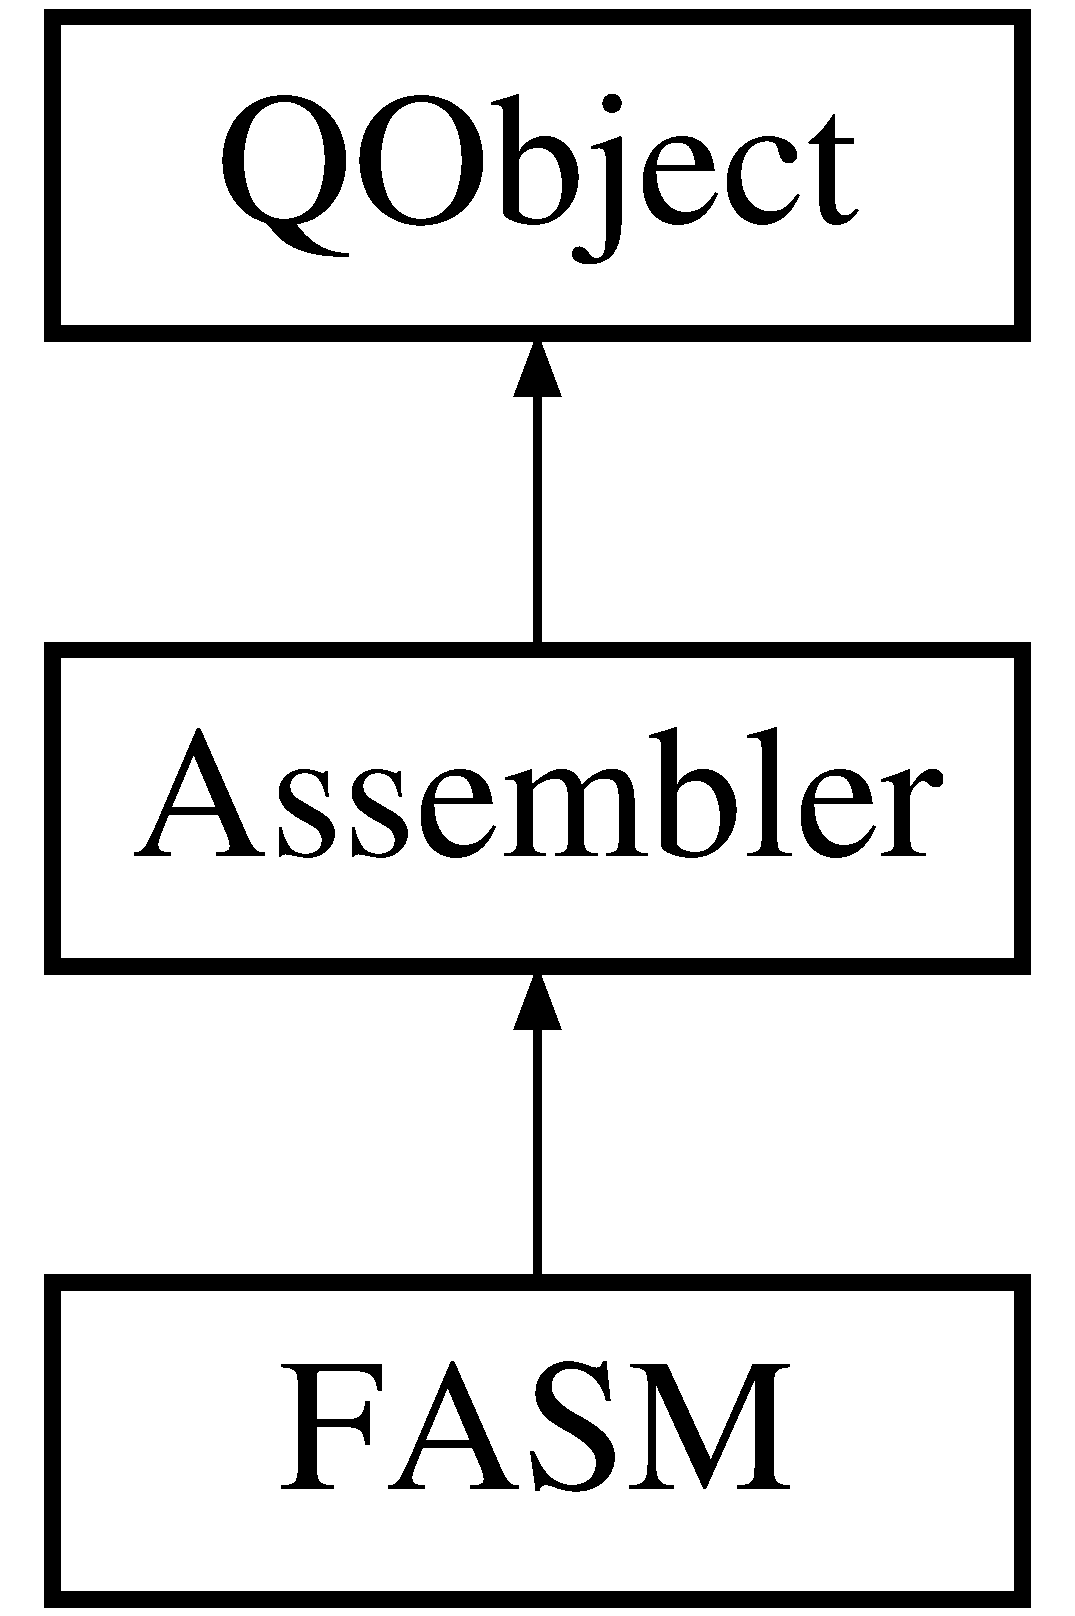
\includegraphics[height=3.000000cm]{class_f_a_s_m}
\end{center}
\end{figure}
\subsection*{Public Member Functions}
\begin{DoxyCompactItemize}
\item 
\hypertarget{class_f_a_s_m_ac7adb4bd7c11ce721b2259e92be18ecf}{}{\bfseries F\+A\+S\+M} (bool x86, Q\+Object $\ast$parent=0)\label{class_f_a_s_m_ac7adb4bd7c11ce721b2259e92be18ecf}

\item 
\hypertarget{class_f_a_s_m_a58a7917ea0f91d68e65b6129d3340194}{}Q\+String \hyperlink{class_f_a_s_m_a58a7917ea0f91d68e65b6129d3340194}{get\+Assembler\+Path} ()\label{class_f_a_s_m_a58a7917ea0f91d68e65b6129d3340194}

\begin{DoxyCompactList}\small\item\em Return the default path to the assembler. \end{DoxyCompactList}\item 
\hypertarget{class_f_a_s_m_aa73825b1d8255e03423cdbbfb0012b9f}{}Q\+String \hyperlink{class_f_a_s_m_aa73825b1d8255e03423cdbbfb0012b9f}{get\+Linker\+Path} ()\label{class_f_a_s_m_aa73825b1d8255e03423cdbbfb0012b9f}

\begin{DoxyCompactList}\small\item\em Returns the default path to the linker. \end{DoxyCompactList}\item 
quint64 \hyperlink{class_f_a_s_m_ad63b8774910442ec8369db49a57cb7ee}{get\+Main\+Offset} (Q\+File \&lst\+Out, Q\+String entry\+Label)
\item 
void \hyperlink{class_f_a_s_m_aec5ded3222ad063755f28e113bf95e32}{parse\+Lst\+File} (Q\+File \&lst\+Out, Q\+Vector$<$ \hyperlink{struct_assembler_1_1_line_num}{Assembler\+::\+Line\+Num} $>$ \&lines, quint64 offset)
\item 
\hypertarget{class_f_a_s_m_afeafae3bc5ec6cc9949ecbd86bb89148}{}void {\bfseries fill\+Highligher\+Rules} (Q\+Vector$<$ \hyperlink{struct_assembler_1_1_highlighting_rule}{Assembler\+::\+Highlighting\+Rule} $>$ \&highlighting\+Rules, Q\+List$<$ Q\+Text\+Char\+Format $\ast$ $>$ \&formats, bool \&\hyperlink{class_assembler_a8e2ae531c6d59dfea8c7bb90febda262}{multi\+Line\+Comments}, Q\+Reg\+Exp \&comment\+Start\+Expression, Q\+Reg\+Exp \&comment\+End\+Expression)\label{class_f_a_s_m_afeafae3bc5ec6cc9949ecbd86bb89148}

\item 
\hypertarget{class_f_a_s_m_acc88d6cc29358917f095925d91d831cf}{}Q\+String \hyperlink{class_f_a_s_m_acc88d6cc29358917f095925d91d831cf}{get\+Start\+Text} ()\label{class_f_a_s_m_acc88d6cc29358917f095925d91d831cf}

\begin{DoxyCompactList}\small\item\em Return the default start text (default project code) \end{DoxyCompactList}\item 
\hypertarget{class_f_a_s_m_a1e912edf8fb4e1d229c4f96089a75118}{}void \hyperlink{class_f_a_s_m_a1e912edf8fb4e1d229c4f96089a75118}{put\+Debug\+String} (\hyperlink{class_code_editor}{Code\+Editor} $\ast$code)\label{class_f_a_s_m_a1e912edf8fb4e1d229c4f96089a75118}

\begin{DoxyCompactList}\small\item\em Puts the debug string that makes frame (mov ebp, esp) \end{DoxyCompactList}\item 
\hypertarget{class_f_a_s_m_aa5c0613929b1ef1feaadb37e199375a5}{}Q\+String \hyperlink{class_f_a_s_m_aa5c0613929b1ef1feaadb37e199375a5}{get\+Assembler\+Options} ()\label{class_f_a_s_m_aa5c0613929b1ef1feaadb37e199375a5}

\begin{DoxyCompactList}\small\item\em Returns the default assembler options. \end{DoxyCompactList}\item 
\hypertarget{class_f_a_s_m_a8739150ad8abe0f9467c406e2d7f999f}{}Q\+String \hyperlink{class_f_a_s_m_a8739150ad8abe0f9467c406e2d7f999f}{get\+Linker\+Options} ()\label{class_f_a_s_m_a8739150ad8abe0f9467c406e2d7f999f}

\begin{DoxyCompactList}\small\item\em Returns the default linker options. \end{DoxyCompactList}\item 
\hypertarget{class_f_a_s_m_aa6c068b5c4cda6b6d67f199fed86fa57}{}Q\+String {\bfseries get\+Listing\+File\+Path} (Q\+File \&lst\+Out)\label{class_f_a_s_m_aa6c068b5c4cda6b6d67f199fed86fa57}

\end{DoxyCompactItemize}
\subsection*{Additional Inherited Members}


\subsection{Detailed Description}
This class defines the behavior for the \hyperlink{class_f_a_s_m}{F\+A\+S\+M} assembler. 



\subsection{Member Function Documentation}
\hypertarget{class_f_a_s_m_ad63b8774910442ec8369db49a57cb7ee}{}\index{F\+A\+S\+M@{F\+A\+S\+M}!get\+Main\+Offset@{get\+Main\+Offset}}
\index{get\+Main\+Offset@{get\+Main\+Offset}!F\+A\+S\+M@{F\+A\+S\+M}}
\subsubsection[{get\+Main\+Offset}]{\setlength{\rightskip}{0pt plus 5cm}quint64 F\+A\+S\+M\+::get\+Main\+Offset (
\begin{DoxyParamCaption}
\item[{Q\+File \&}]{lst, }
\item[{Q\+String}]{entry\+Label}
\end{DoxyParamCaption}
)\hspace{0.3cm}{\ttfamily [virtual]}}\label{class_f_a_s_m_ad63b8774910442ec8369db49a57cb7ee}
get file with listing and name of entry label -\/ main or start. Returns the offset of this label -\/ number of strings and where the label is placed. 

Implements \hyperlink{class_assembler_aa41f46e0cd774718d84bf4e5bd9c65b7}{Assembler}.

\hypertarget{class_f_a_s_m_aec5ded3222ad063755f28e113bf95e32}{}\index{F\+A\+S\+M@{F\+A\+S\+M}!parse\+Lst\+File@{parse\+Lst\+File}}
\index{parse\+Lst\+File@{parse\+Lst\+File}!F\+A\+S\+M@{F\+A\+S\+M}}
\subsubsection[{parse\+Lst\+File}]{\setlength{\rightskip}{0pt plus 5cm}void F\+A\+S\+M\+::parse\+Lst\+File (
\begin{DoxyParamCaption}
\item[{Q\+File \&}]{lst, }
\item[{Q\+Vector$<$ {\bf Assembler\+::\+Line\+Num} $>$ \&}]{lines, }
\item[{quint64}]{offset}
\end{DoxyParamCaption}
)\hspace{0.3cm}{\ttfamily [virtual]}}\label{class_f_a_s_m_aec5ded3222ad063755f28e113bf95e32}
Parses the listing file lst and fills Q\+Vector lines with results of parsing. offset -\/ difference between program code in memory and in file. 

Implements \hyperlink{class_assembler_aa724d277157a407d4d7fd3d0a23e84a7}{Assembler}.



The documentation for this class was generated from the following files\+:\begin{DoxyCompactItemize}
\item 
\hyperlink{fasm_8h}{fasm.\+h}\item 
\hyperlink{fasm_8cpp}{fasm.\+cpp}\end{DoxyCompactItemize}

\hypertarget{class_find_dialog}{}\section{Find\+Dialog Class Reference}
\label{class_find_dialog}\index{Find\+Dialog@{Find\+Dialog}}


This class represents the \char`\"{}find text\char`\"{} functionality.  




{\ttfamily \#include $<$finddialog.\+h$>$}

Inheritance diagram for Find\+Dialog\+:\begin{figure}[H]
\begin{center}
\leavevmode
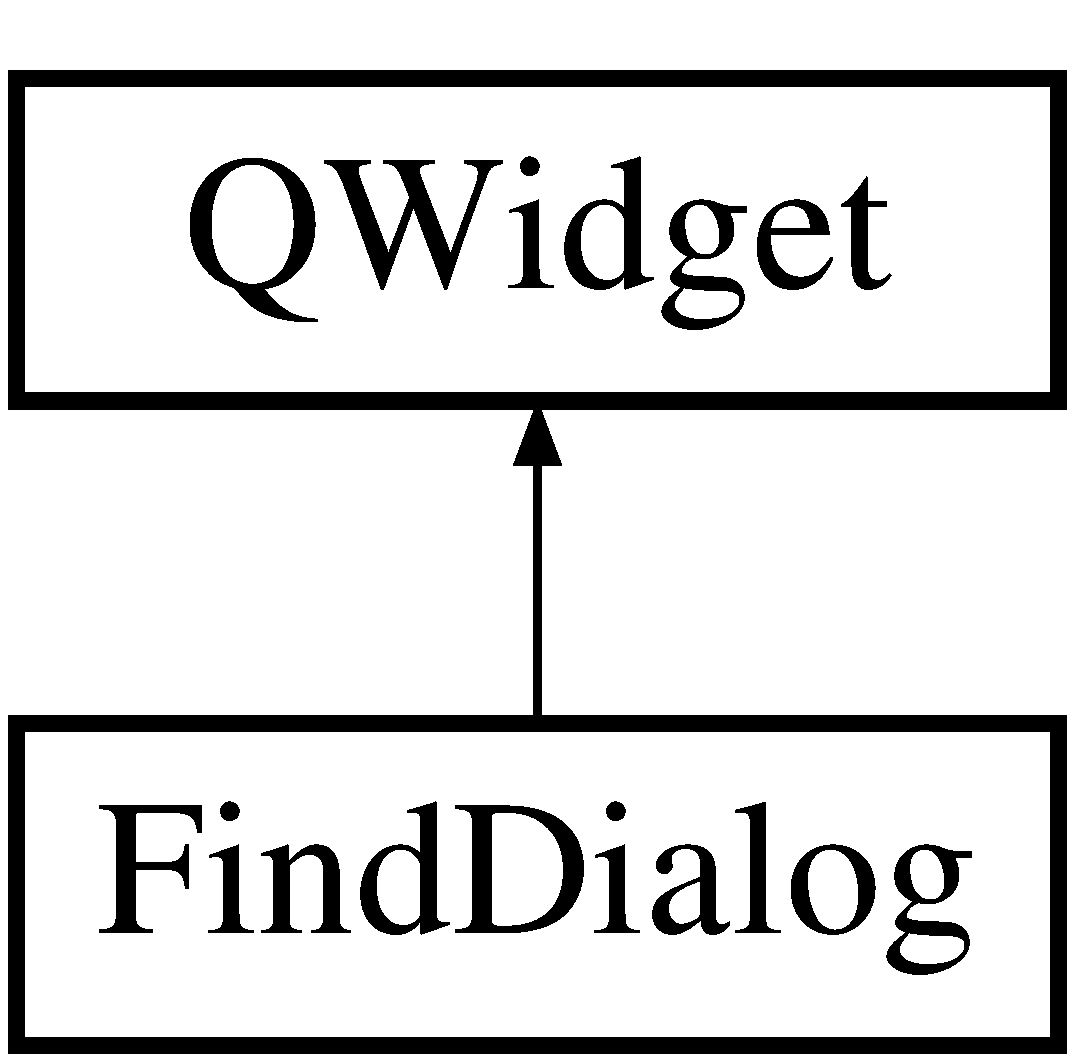
\includegraphics[height=2.000000cm]{class_find_dialog}
\end{center}
\end{figure}
\subsection*{Public Slots}
\begin{DoxyCompactItemize}
\item 
\hypertarget{class_find_dialog_a4c4a3771fb980ba9c69ca6a67f0e0064}{}bool {\bfseries close} ()\label{class_find_dialog_a4c4a3771fb980ba9c69ca6a67f0e0064}

\end{DoxyCompactItemize}
\subsection*{Signals}
\begin{DoxyCompactItemize}
\item 
\hypertarget{class_find_dialog_a3046657833c8120339f3a03444f8e5ff}{}void {\bfseries find\+Next} (const Q\+String \&str, Qt\+::\+Case\+Sensitivity cs, bool all, bool replace, const Q\+String \&replace\+Text=0)\label{class_find_dialog_a3046657833c8120339f3a03444f8e5ff}

\end{DoxyCompactItemize}
\subsection*{Public Member Functions}
\begin{DoxyCompactItemize}
\item 
\hypertarget{class_find_dialog_af9dc0e86bec39e9b3a0b954a603a8e76}{}{\bfseries Find\+Dialog} (Q\+Widget $\ast$parent=0)\label{class_find_dialog_af9dc0e86bec39e9b3a0b954a603a8e76}

\item 
\hypertarget{class_find_dialog_a966e7ab89d607dbff17d17a95f102587}{}void {\bfseries close\+Event} (Q\+Close\+Event $\ast$e)\label{class_find_dialog_a966e7ab89d607dbff17d17a95f102587}

\end{DoxyCompactItemize}
\subsection*{Private Slots}
\begin{DoxyCompactItemize}
\item 
\hypertarget{class_find_dialog_a655e40bfdcc2c7712a1541bbf8cf2744}{}void {\bfseries find\+Clicked} ()\label{class_find_dialog_a655e40bfdcc2c7712a1541bbf8cf2744}

\item 
\hypertarget{class_find_dialog_aa42a9c9abe4a4ede6d87b2da08b3b928}{}void {\bfseries find\+All\+Clicked} ()\label{class_find_dialog_aa42a9c9abe4a4ede6d87b2da08b3b928}

\item 
\hypertarget{class_find_dialog_ae70c0cd7fbfa8b635e2bf43c34ee6586}{}void {\bfseries replace\+Clicked} ()\label{class_find_dialog_ae70c0cd7fbfa8b635e2bf43c34ee6586}

\item 
\hypertarget{class_find_dialog_abe5173da17631afacde0742e4cd9e471}{}void {\bfseries replace\+All\+Clicked} ()\label{class_find_dialog_abe5173da17631afacde0742e4cd9e471}

\item 
\hypertarget{class_find_dialog_a2f659549e817833ee65d14f81d59cced}{}void {\bfseries enable\+Find\+Button} (const Q\+String \&text)\label{class_find_dialog_a2f659549e817833ee65d14f81d59cced}

\end{DoxyCompactItemize}
\subsection*{Private Attributes}
\begin{DoxyCompactItemize}
\item 
\hypertarget{class_find_dialog_a162cc453e71d917ac08d1aabbdbf4fbd}{}Q\+Label $\ast$ {\bfseries search\+Label}\label{class_find_dialog_a162cc453e71d917ac08d1aabbdbf4fbd}

\item 
\hypertarget{class_find_dialog_aa29766ac87487026ac7a76951e4b8d0b}{}Q\+Label $\ast$ {\bfseries replace\+Label}\label{class_find_dialog_aa29766ac87487026ac7a76951e4b8d0b}

\item 
\hypertarget{class_find_dialog_ac516bb12976237f707d7b9c51738d73e}{}Q\+Line\+Edit $\ast$ {\bfseries search\+Edit}\label{class_find_dialog_ac516bb12976237f707d7b9c51738d73e}

\item 
\hypertarget{class_find_dialog_a343258a37f12d131051ad3cbdf353a28}{}Q\+Line\+Edit $\ast$ {\bfseries replace\+Edit}\label{class_find_dialog_a343258a37f12d131051ad3cbdf353a28}

\item 
\hypertarget{class_find_dialog_a35f7083798170a5d572fc9d869ca6d1a}{}Q\+Check\+Box $\ast$ {\bfseries case\+Check\+Box}\label{class_find_dialog_a35f7083798170a5d572fc9d869ca6d1a}

\item 
\hypertarget{class_find_dialog_a2a4e97929c23e98e150924d7420a481f}{}Q\+Push\+Button $\ast$ {\bfseries find\+Button}\label{class_find_dialog_a2a4e97929c23e98e150924d7420a481f}

\item 
\hypertarget{class_find_dialog_aa0bd8a47a2074da69056fbf812ea7811}{}Q\+Push\+Button $\ast$ {\bfseries find\+All\+Button}\label{class_find_dialog_aa0bd8a47a2074da69056fbf812ea7811}

\item 
\hypertarget{class_find_dialog_a671d60112b89dea510c149372d2992ef}{}Q\+Push\+Button $\ast$ {\bfseries replace\+Button}\label{class_find_dialog_a671d60112b89dea510c149372d2992ef}

\item 
\hypertarget{class_find_dialog_a558408ab812aebae4a63f805a3951023}{}Q\+Push\+Button $\ast$ {\bfseries replace\+All\+Button}\label{class_find_dialog_a558408ab812aebae4a63f805a3951023}

\item 
\hypertarget{class_find_dialog_a4cd1160790eb513e0a103ad286fc2510}{}Q\+Push\+Button $\ast$ {\bfseries close\+Button}\label{class_find_dialog_a4cd1160790eb513e0a103ad286fc2510}

\item 
\hypertarget{class_find_dialog_a891b70d2a9b9adeae41b20298e7d23cc}{}Q\+H\+Box\+Layout $\ast$ {\bfseries replace\+Layout}\label{class_find_dialog_a891b70d2a9b9adeae41b20298e7d23cc}

\item 
\hypertarget{class_find_dialog_acebe70639dab551c763cfe19cab7f9ce}{}Q\+H\+Box\+Layout $\ast$ {\bfseries search\+Layout}\label{class_find_dialog_acebe70639dab551c763cfe19cab7f9ce}

\item 
\hypertarget{class_find_dialog_a130675f44fd1bd0fda090793fdf5bff6}{}Q\+H\+Box\+Layout $\ast$ {\bfseries replace\+Button\+Layout}\label{class_find_dialog_a130675f44fd1bd0fda090793fdf5bff6}

\item 
\hypertarget{class_find_dialog_a735dfeee149248594b8311c234866df7}{}Q\+V\+Box\+Layout $\ast$ {\bfseries left\+Layout}\label{class_find_dialog_a735dfeee149248594b8311c234866df7}

\item 
\hypertarget{class_find_dialog_ab93f0e33031fb7dbe6f55f2de1f364aa}{}Q\+V\+Box\+Layout $\ast$ {\bfseries right\+Layout}\label{class_find_dialog_ab93f0e33031fb7dbe6f55f2de1f364aa}

\item 
\hypertarget{class_find_dialog_aae801e97a136a56b3e936b312837ce07}{}Q\+H\+Box\+Layout $\ast$ {\bfseries main\+Layout}\label{class_find_dialog_aae801e97a136a56b3e936b312837ce07}

\item 
\hypertarget{class_find_dialog_a0d031ef966bb68201131d8360ed502ba}{}Q\+Spacer\+Item $\ast$ {\bfseries search\+Spacer}\label{class_find_dialog_a0d031ef966bb68201131d8360ed502ba}

\end{DoxyCompactItemize}


\subsection{Detailed Description}
This class represents the \char`\"{}find text\char`\"{} functionality. 

All of the methods including Find Find All Find\&Replace Are defined here. 

The documentation for this class was generated from the following files\+:\begin{DoxyCompactItemize}
\item 
\hyperlink{finddialog_8h}{finddialog.\+h}\item 
\hyperlink{finddialog_8cpp}{finddialog.\+cpp}\end{DoxyCompactItemize}

\hypertarget{class_g_a_s}{}\section{G\+A\+S Class Reference}
\label{class_g_a_s}\index{G\+A\+S@{G\+A\+S}}


This class defines the behavior for the \hyperlink{class_g_a_s}{G\+A\+S} assembler.  




{\ttfamily \#include $<$gas.\+h$>$}

Inheritance diagram for G\+A\+S\+:\begin{figure}[H]
\begin{center}
\leavevmode
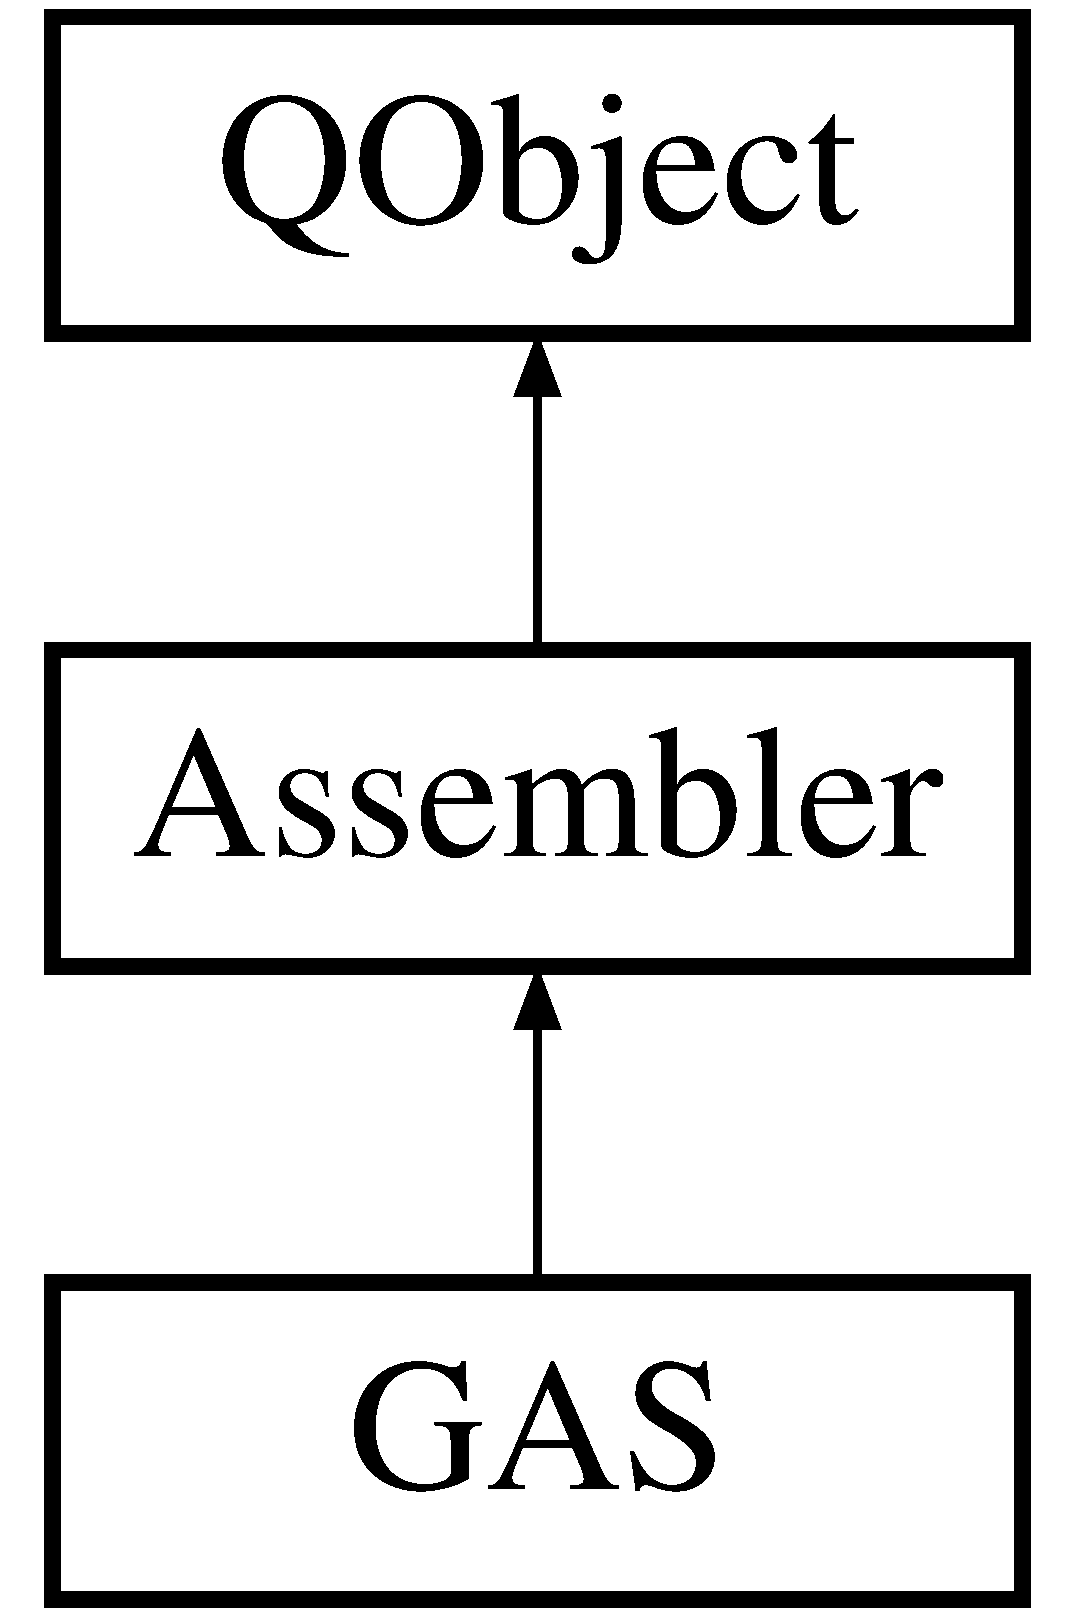
\includegraphics[height=3.000000cm]{class_g_a_s}
\end{center}
\end{figure}
\subsection*{Public Member Functions}
\begin{DoxyCompactItemize}
\item 
\hypertarget{class_g_a_s_af13f9f492a83b6a8d13607e2dbc08726}{}{\bfseries G\+A\+S} (bool x86, Q\+Object $\ast$parent=0)\label{class_g_a_s_af13f9f492a83b6a8d13607e2dbc08726}

\item 
\hypertarget{class_g_a_s_adc206282c20b7a3f69b40c294883c1f0}{}Q\+String \hyperlink{class_g_a_s_adc206282c20b7a3f69b40c294883c1f0}{get\+Assembler\+Path} ()\label{class_g_a_s_adc206282c20b7a3f69b40c294883c1f0}

\begin{DoxyCompactList}\small\item\em Return the default path to the assembler. \end{DoxyCompactList}\item 
\hypertarget{class_g_a_s_a21833928db55133bad977fca971fad3a}{}Q\+String \hyperlink{class_g_a_s_a21833928db55133bad977fca971fad3a}{get\+Linker\+Path} ()\label{class_g_a_s_a21833928db55133bad977fca971fad3a}

\begin{DoxyCompactList}\small\item\em Returns the default path to the linker. \end{DoxyCompactList}\item 
quint64 \hyperlink{class_g_a_s_ab1d4e22ffd3a438afa4dad4025ab2735}{get\+Main\+Offset} (Q\+File \&lst, Q\+String entry\+Label)
\item 
void \hyperlink{class_g_a_s_a572e0d7058f6f5d65a90c77a8b727460}{parse\+Lst\+File} (Q\+File \&lst, Q\+Vector$<$ \hyperlink{struct_assembler_1_1_line_num}{Assembler\+::\+Line\+Num} $>$ \&lines, quint64 offset)
\item 
\hypertarget{class_g_a_s_a50f67e9e0a7a5d235397bee4cc05a2a0}{}void {\bfseries fill\+Highligher\+Rules} (Q\+Vector$<$ \hyperlink{struct_assembler_1_1_highlighting_rule}{Assembler\+::\+Highlighting\+Rule} $>$ \&highlighting\+Rules, Q\+List$<$ Q\+Text\+Char\+Format $\ast$ $>$ \&formats, bool \&\hyperlink{class_assembler_a8e2ae531c6d59dfea8c7bb90febda262}{multi\+Line\+Comments}, Q\+Reg\+Exp \&comment\+Start\+Expression, Q\+Reg\+Exp \&comment\+End\+Expression)\label{class_g_a_s_a50f67e9e0a7a5d235397bee4cc05a2a0}

\item 
\hypertarget{class_g_a_s_aeb1894b36402e608ac97ce73547f51bd}{}Q\+String \hyperlink{class_g_a_s_aeb1894b36402e608ac97ce73547f51bd}{get\+Start\+Text} ()\label{class_g_a_s_aeb1894b36402e608ac97ce73547f51bd}

\begin{DoxyCompactList}\small\item\em Return the default start text (default project code) \end{DoxyCompactList}\item 
\hypertarget{class_g_a_s_ae5477b2cccdb69b665be5d183d6b7086}{}void \hyperlink{class_g_a_s_ae5477b2cccdb69b665be5d183d6b7086}{put\+Debug\+String} (\hyperlink{class_code_editor}{Code\+Editor} $\ast$code)\label{class_g_a_s_ae5477b2cccdb69b665be5d183d6b7086}

\begin{DoxyCompactList}\small\item\em Puts the debug string that makes frame (mov ebp, esp) \end{DoxyCompactList}\item 
\hypertarget{class_g_a_s_af74e0b595c4ac405ba75895f7aadeb66}{}Q\+String \hyperlink{class_g_a_s_af74e0b595c4ac405ba75895f7aadeb66}{get\+Assembler\+Options} ()\label{class_g_a_s_af74e0b595c4ac405ba75895f7aadeb66}

\begin{DoxyCompactList}\small\item\em Returns the default assembler options. \end{DoxyCompactList}\item 
\hypertarget{class_g_a_s_a127305521d703d7cca95a087a220d9f0}{}Q\+String \hyperlink{class_g_a_s_a127305521d703d7cca95a087a220d9f0}{get\+Linker\+Options} ()\label{class_g_a_s_a127305521d703d7cca95a087a220d9f0}

\begin{DoxyCompactList}\small\item\em Returns the default linker options. \end{DoxyCompactList}\end{DoxyCompactItemize}
\subsection*{Additional Inherited Members}


\subsection{Detailed Description}
This class defines the behavior for the \hyperlink{class_g_a_s}{G\+A\+S} assembler. 



\subsection{Member Function Documentation}
\hypertarget{class_g_a_s_ab1d4e22ffd3a438afa4dad4025ab2735}{}\index{G\+A\+S@{G\+A\+S}!get\+Main\+Offset@{get\+Main\+Offset}}
\index{get\+Main\+Offset@{get\+Main\+Offset}!G\+A\+S@{G\+A\+S}}
\subsubsection[{get\+Main\+Offset}]{\setlength{\rightskip}{0pt plus 5cm}quint64 G\+A\+S\+::get\+Main\+Offset (
\begin{DoxyParamCaption}
\item[{Q\+File \&}]{lst, }
\item[{Q\+String}]{entry\+Label}
\end{DoxyParamCaption}
)\hspace{0.3cm}{\ttfamily [virtual]}}\label{class_g_a_s_ab1d4e22ffd3a438afa4dad4025ab2735}
get file with listing and name of entry label -\/ main or start. Returns the offset of this label -\/ number of strings and where the label is placed. 

Implements \hyperlink{class_assembler_aa41f46e0cd774718d84bf4e5bd9c65b7}{Assembler}.

\hypertarget{class_g_a_s_a572e0d7058f6f5d65a90c77a8b727460}{}\index{G\+A\+S@{G\+A\+S}!parse\+Lst\+File@{parse\+Lst\+File}}
\index{parse\+Lst\+File@{parse\+Lst\+File}!G\+A\+S@{G\+A\+S}}
\subsubsection[{parse\+Lst\+File}]{\setlength{\rightskip}{0pt plus 5cm}void G\+A\+S\+::parse\+Lst\+File (
\begin{DoxyParamCaption}
\item[{Q\+File \&}]{lst, }
\item[{Q\+Vector$<$ {\bf Assembler\+::\+Line\+Num} $>$ \&}]{lines, }
\item[{quint64}]{offset}
\end{DoxyParamCaption}
)\hspace{0.3cm}{\ttfamily [virtual]}}\label{class_g_a_s_a572e0d7058f6f5d65a90c77a8b727460}
Parses the listing file lst and fills Q\+Vector lines with results of parsing. offset -\/ difference between program code in memory and in file. 

Implements \hyperlink{class_assembler_aa724d277157a407d4d7fd3d0a23e84a7}{Assembler}.



The documentation for this class was generated from the following files\+:\begin{DoxyCompactItemize}
\item 
\hyperlink{gas_8h}{gas.\+h}\item 
\hyperlink{gas_8cpp}{gas.\+cpp}\end{DoxyCompactItemize}

\hypertarget{class_get_started_widget}{}\section{Get\+Started\+Widget Class Reference}
\label{class_get_started_widget}\index{Get\+Started\+Widget@{Get\+Started\+Widget}}
Inheritance diagram for Get\+Started\+Widget\+:\begin{figure}[H]
\begin{center}
\leavevmode
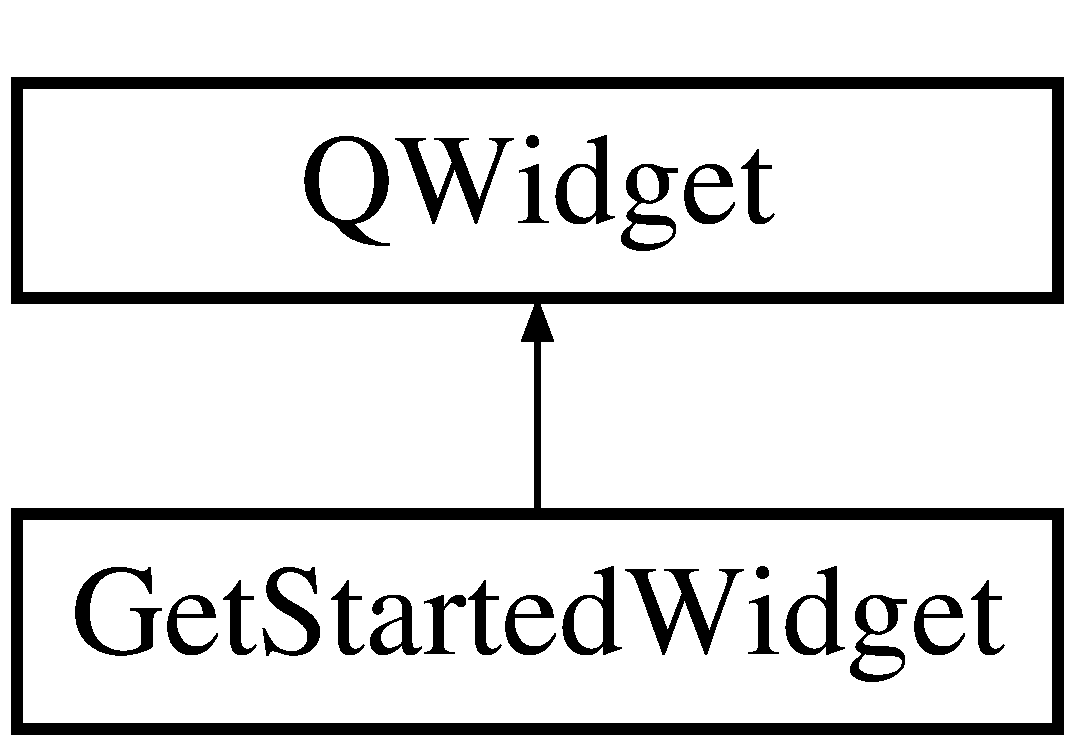
\includegraphics[height=2.000000cm]{class_get_started_widget}
\end{center}
\end{figure}
\subsection*{Public Member Functions}
\begin{DoxyCompactItemize}
\item 
\hypertarget{class_get_started_widget_a9cfb08d5e11309e0af9e8711a09adffa}{}{\bfseries Get\+Started\+Widget} (Q\+Widget $\ast$parent=0)\label{class_get_started_widget_a9cfb08d5e11309e0af9e8711a09adffa}

\end{DoxyCompactItemize}
\subsection*{Public Attributes}
\begin{DoxyCompactItemize}
\item 
\hypertarget{class_get_started_widget_af23faf9268f1e4632084bba304c85c36}{}Q\+Command\+Link\+Button $\ast$ {\bfseries new\+Button}\label{class_get_started_widget_af23faf9268f1e4632084bba304c85c36}

\item 
\hypertarget{class_get_started_widget_a2cc201c00b37e685949d614f8bf29df8}{}Q\+Command\+Link\+Button $\ast$ {\bfseries open\+Button}\label{class_get_started_widget_a2cc201c00b37e685949d614f8bf29df8}

\item 
\hypertarget{class_get_started_widget_a91a3519b78e9cf1012f0119299b7af42}{}Q\+Command\+Link\+Button $\ast$ {\bfseries prev\+Session\+Button}\label{class_get_started_widget_a91a3519b78e9cf1012f0119299b7af42}

\end{DoxyCompactItemize}
\subsection*{Private Attributes}
\begin{DoxyCompactItemize}
\item 
\hypertarget{class_get_started_widget_a967f3dadf71419dad0337e76a4700085}{}Q\+H\+Box\+Layout $\ast$ {\bfseries label\+Layout}\label{class_get_started_widget_a967f3dadf71419dad0337e76a4700085}

\item 
\hypertarget{class_get_started_widget_aed1b1611fa79fea98f289be0927aeb13}{}Q\+V\+Box\+Layout $\ast$ {\bfseries layout}\label{class_get_started_widget_aed1b1611fa79fea98f289be0927aeb13}

\item 
\hypertarget{class_get_started_widget_a2c001e9a29d232afbf5185097a97b481}{}Q\+Label $\ast$ {\bfseries welcome\+Label}\label{class_get_started_widget_a2c001e9a29d232afbf5185097a97b481}

\item 
\hypertarget{class_get_started_widget_a00139a801f4614d47189081e71e6f932}{}Q\+Label $\ast$ {\bfseries img\+Label}\label{class_get_started_widget_a00139a801f4614d47189081e71e6f932}

\item 
\hypertarget{class_get_started_widget_a7fd3a6ac1bac6e326b8dab87ee313b52}{}Q\+Spacer\+Item $\ast$ {\bfseries spacer}\label{class_get_started_widget_a7fd3a6ac1bac6e326b8dab87ee313b52}

\item 
\hypertarget{class_get_started_widget_aa697f30ca3a5facd85e4a70e98001c65}{}Q\+Spacer\+Item $\ast$ {\bfseries bottom\+Spacer}\label{class_get_started_widget_aa697f30ca3a5facd85e4a70e98001c65}

\item 
\hypertarget{class_get_started_widget_ac5e0e935d94b17e251cea738c920bd66}{}Q\+Spacer\+Item $\ast$ {\bfseries left\+Spacer}\label{class_get_started_widget_ac5e0e935d94b17e251cea738c920bd66}

\end{DoxyCompactItemize}


The documentation for this class was generated from the following files\+:\begin{DoxyCompactItemize}
\item 
\hyperlink{getstartedwidget_8h}{getstartedwidget.\+h}\item 
\hyperlink{getstartedwidget_8cpp}{getstartedwidget.\+cpp}\end{DoxyCompactItemize}

\hypertarget{class_highlighter}{}\section{Highlighter Class Reference}
\label{class_highlighter}\index{Highlighter@{Highlighter}}


This class defines the rules of syntax highlighting.  




{\ttfamily \#include $<$highlighter.\+h$>$}

Inheritance diagram for Highlighter\+:\begin{figure}[H]
\begin{center}
\leavevmode
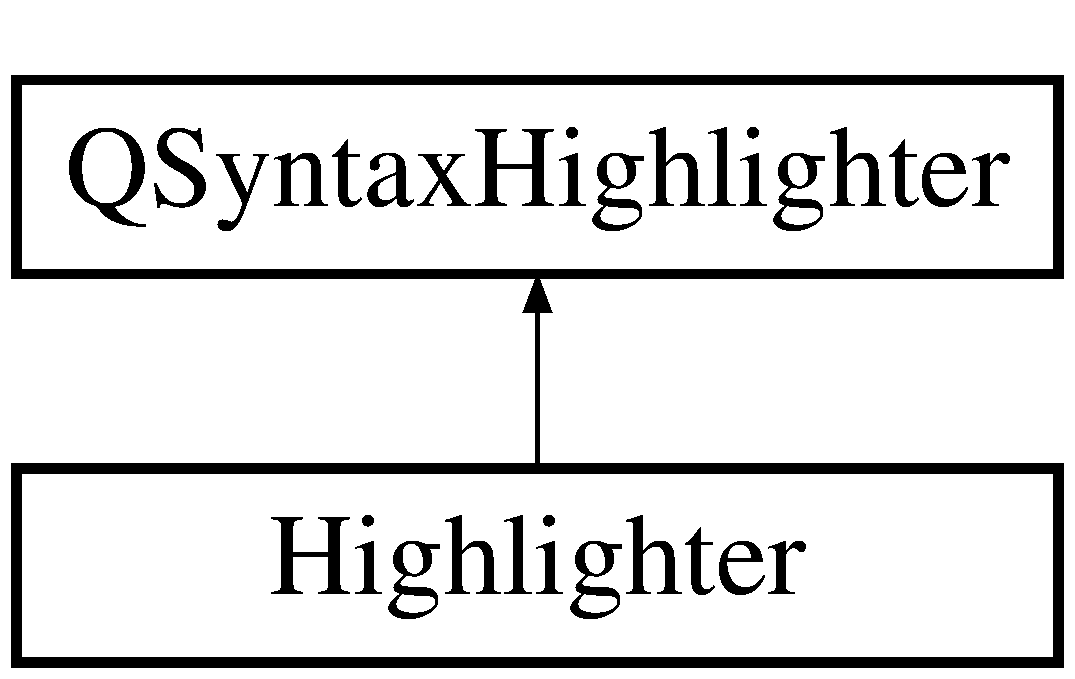
\includegraphics[height=2.000000cm]{class_highlighter}
\end{center}
\end{figure}
\subsection*{Public Member Functions}
\begin{DoxyCompactItemize}
\item 
\hypertarget{class_highlighter_a5e7fcc335ddbe9516c144e2fdff46e3c}{}{\bfseries Highlighter} (\hyperlink{class_assembler}{Assembler} $\ast$assembler, Q\+Text\+Document $\ast$parent=0)\label{class_highlighter_a5e7fcc335ddbe9516c144e2fdff46e3c}

\end{DoxyCompactItemize}
\subsection*{Protected Member Functions}
\begin{DoxyCompactItemize}
\item 
\hypertarget{class_highlighter_ad07c7fd55d2ce2c675bca607b9370488}{}void {\bfseries highlight\+Block} (const Q\+String \&text)\label{class_highlighter_ad07c7fd55d2ce2c675bca607b9370488}

\end{DoxyCompactItemize}
\subsection*{Private Types}
\begin{DoxyCompactItemize}
\item 
\hypertarget{class_highlighter_aa60f8c7c52decbe57b9f5ba4705402e2}{}typedef \hyperlink{struct_assembler_1_1_highlighting_rule}{Assembler\+::\+Highlighting\+Rule} {\bfseries Highlighting\+Rule}\label{class_highlighter_aa60f8c7c52decbe57b9f5ba4705402e2}

\end{DoxyCompactItemize}
\subsection*{Private Member Functions}
\begin{DoxyCompactItemize}
\item 
\hypertarget{class_highlighter_a17ed99316195809e6bb92711a959eecf}{}bool {\bfseries is\+Comment\+In\+Quote} (const Q\+String \&text, int index)\label{class_highlighter_a17ed99316195809e6bb92711a959eecf}

\end{DoxyCompactItemize}
\subsection*{Private Attributes}
\begin{DoxyCompactItemize}
\item 
\hypertarget{class_highlighter_aa23f8b3f4ddd1354f508b46d77897fe5}{}Q\+Vector$<$ \hyperlink{struct_assembler_1_1_highlighting_rule}{Highlighting\+Rule} $>$ {\bfseries highlighting\+Rules}\label{class_highlighter_aa23f8b3f4ddd1354f508b46d77897fe5}

\item 
\hypertarget{class_highlighter_a67cdecd667929b4eefbc7057d58cd90b}{}Q\+Reg\+Exp {\bfseries comment\+Start\+Expression}\label{class_highlighter_a67cdecd667929b4eefbc7057d58cd90b}

\item 
\hypertarget{class_highlighter_a3baa1033bbdf70a16df42940968b72b4}{}Q\+Reg\+Exp {\bfseries comment\+End\+Expression}\label{class_highlighter_a3baa1033bbdf70a16df42940968b72b4}

\item 
\hypertarget{class_highlighter_ad4ea108a70fbf74e69439a35261fb36b}{}bool {\bfseries multi\+Line\+Comments}\label{class_highlighter_ad4ea108a70fbf74e69439a35261fb36b}

\item 
\hypertarget{class_highlighter_a1b7ef37cb63af92ab17f91885922418d}{}Q\+Text\+Char\+Format {\bfseries comment\+Format}\label{class_highlighter_a1b7ef37cb63af92ab17f91885922418d}

\end{DoxyCompactItemize}


\subsection{Detailed Description}
This class defines the rules of syntax highlighting. 

Because some assemblers use different keywords, it is essential to distinguish between rules. Each rule set is defined as a \hyperlink{class_highlighter}{Highlighter} instance. 

The documentation for this class was generated from the following files\+:\begin{DoxyCompactItemize}
\item 
\hyperlink{highlighter_8h}{highlighter.\+h}\item 
\hyperlink{highlighter_8cpp}{highlighter.\+cpp}\end{DoxyCompactItemize}

\hypertarget{struct_assembler_1_1_highlighting_rule}{}\section{Assembler\+:\+:Highlighting\+Rule Struct Reference}
\label{struct_assembler_1_1_highlighting_rule}\index{Assembler\+::\+Highlighting\+Rule@{Assembler\+::\+Highlighting\+Rule}}
\subsection*{Public Attributes}
\begin{DoxyCompactItemize}
\item 
\hypertarget{struct_assembler_1_1_highlighting_rule_aa3ba772c482811abece37b73b007eef3}{}Q\+Reg\+Exp \hyperlink{struct_assembler_1_1_highlighting_rule_aa3ba772c482811abece37b73b007eef3}{pattern}\label{struct_assembler_1_1_highlighting_rule_aa3ba772c482811abece37b73b007eef3}

\begin{DoxyCompactList}\small\item\em Pattern to highlight. \end{DoxyCompactList}\item 
\hypertarget{struct_assembler_1_1_highlighting_rule_ac31c4c54be807ed0c1cebf5478316bc3}{}Q\+Text\+Char\+Format \hyperlink{struct_assembler_1_1_highlighting_rule_ac31c4c54be807ed0c1cebf5478316bc3}{format}\label{struct_assembler_1_1_highlighting_rule_ac31c4c54be807ed0c1cebf5478316bc3}

\begin{DoxyCompactList}\small\item\em Whighlighting format U\+N\+K\+N\+O\+W\+N F\+I\+L\+L T\+H\+I\+S I\+N. \end{DoxyCompactList}\item 
\hypertarget{struct_assembler_1_1_highlighting_rule_acec02296231600d74137df651f987808}{}bool {\bfseries is\+Comment}\label{struct_assembler_1_1_highlighting_rule_acec02296231600d74137df651f987808}

\end{DoxyCompactItemize}


The documentation for this struct was generated from the following file\+:\begin{DoxyCompactItemize}
\item 
\hyperlink{assembler_8h}{assembler.\+h}\end{DoxyCompactItemize}

\hypertarget{struct_assembler_1_1_line_num}{}\section{Assembler\+:\+:Line\+Num Struct Reference}
\label{struct_assembler_1_1_line_num}\index{Assembler\+::\+Line\+Num@{Assembler\+::\+Line\+Num}}
\subsection*{Public Member Functions}
\begin{DoxyCompactItemize}
\item 
\hypertarget{struct_assembler_1_1_line_num_af687ddb816dcd5c29f896cae92e6d7b5}{}bool {\bfseries operator==} (const \hyperlink{struct_assembler_1_1_line_num}{Line\+Num} \&ln)\label{struct_assembler_1_1_line_num_af687ddb816dcd5c29f896cae92e6d7b5}

\end{DoxyCompactItemize}
\subsection*{Public Attributes}
\begin{DoxyCompactItemize}
\item 
\hypertarget{struct_assembler_1_1_line_num_ae5d6969a723ee8e06940233863fcd8e4}{}quint64 \hyperlink{struct_assembler_1_1_line_num_ae5d6969a723ee8e06940233863fcd8e4}{num\+In\+Code}\label{struct_assembler_1_1_line_num_ae5d6969a723ee8e06940233863fcd8e4}

\begin{DoxyCompactList}\small\item\em String number in code in S\+A\+S\+M code area -\/$>$What does string number in code mean? \end{DoxyCompactList}\item 
\hypertarget{struct_assembler_1_1_line_num_a6ae7b98e18a63f558aff59cce0810aac}{}quint64 \hyperlink{struct_assembler_1_1_line_num_a6ae7b98e18a63f558aff59cce0810aac}{num\+In\+Mem}\label{struct_assembler_1_1_line_num_a6ae7b98e18a63f558aff59cce0810aac}

\begin{DoxyCompactList}\small\item\em Address of instruction in memory -\/$>$ which instruction? Of the user's? \end{DoxyCompactList}\end{DoxyCompactItemize}


The documentation for this struct was generated from the following file\+:\begin{DoxyCompactItemize}
\item 
\hyperlink{assembler_8h}{assembler.\+h}\end{DoxyCompactItemize}

\hypertarget{class_line_number_area}{}\section{Line\+Number\+Area Class Reference}
\label{class_line_number_area}\index{Line\+Number\+Area@{Line\+Number\+Area}}
Inheritance diagram for Line\+Number\+Area\+:\begin{figure}[H]
\begin{center}
\leavevmode
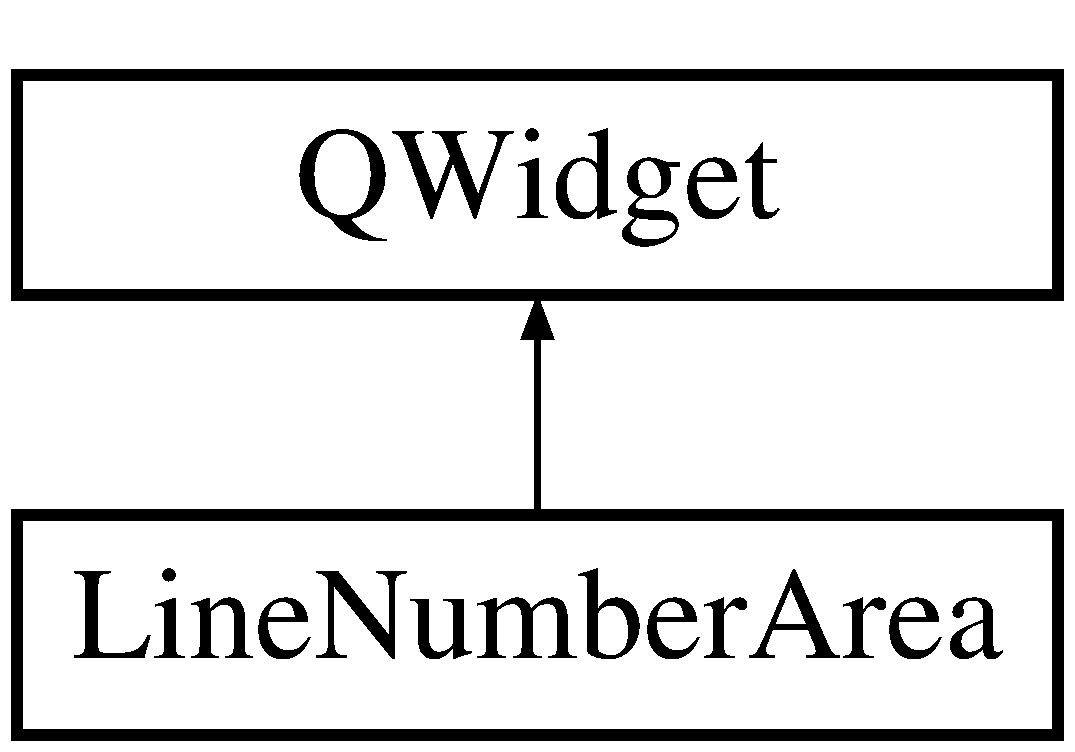
\includegraphics[height=2.000000cm]{class_line_number_area}
\end{center}
\end{figure}
\subsection*{Public Member Functions}
\begin{DoxyCompactItemize}
\item 
\hypertarget{class_line_number_area_afc09bd40180955642bf5fc3ae2e41ecc}{}{\bfseries Line\+Number\+Area} (\hyperlink{class_code_editor}{Code\+Editor} $\ast$editor)\label{class_line_number_area_afc09bd40180955642bf5fc3ae2e41ecc}

\item 
\hypertarget{class_line_number_area_a5d31f7fb107bc1eefd7ae4974c095308}{}Q\+Size {\bfseries size\+Hint} () const \label{class_line_number_area_a5d31f7fb107bc1eefd7ae4974c095308}

\end{DoxyCompactItemize}
\subsection*{Protected Member Functions}
\begin{DoxyCompactItemize}
\item 
\hypertarget{class_line_number_area_a56400934bfe272427deb3ffd975b3a7f}{}void {\bfseries paint\+Event} (Q\+Paint\+Event $\ast$event)\label{class_line_number_area_a56400934bfe272427deb3ffd975b3a7f}

\item 
\hypertarget{class_line_number_area_a856443cc79937f836ed2e9bbae3cb118}{}void {\bfseries mouse\+Press\+Event} (Q\+Mouse\+Event $\ast$event)\label{class_line_number_area_a856443cc79937f836ed2e9bbae3cb118}

\end{DoxyCompactItemize}
\subsection*{Private Attributes}
\begin{DoxyCompactItemize}
\item 
\hypertarget{class_line_number_area_ae1dcaf51cd365f6137d1beecc1e5af80}{}\hyperlink{class_code_editor}{Code\+Editor} $\ast$ {\bfseries code\+Editor}\label{class_line_number_area_ae1dcaf51cd365f6137d1beecc1e5af80}

\end{DoxyCompactItemize}


The documentation for this class was generated from the following file\+:\begin{DoxyCompactItemize}
\item 
\hyperlink{codeeditor_8h}{codeeditor.\+h}\end{DoxyCompactItemize}

\hypertarget{class_main_window}{}\section{Main\+Window Class Reference}
\label{class_main_window}\index{Main\+Window@{Main\+Window}}


The \hyperlink{class_main_window}{Main\+Window} class defines the actions and behavior of the main user interface.  




{\ttfamily \#include $<$mainwindow.\+h$>$}

Inheritance diagram for Main\+Window\+:\begin{figure}[H]
\begin{center}
\leavevmode
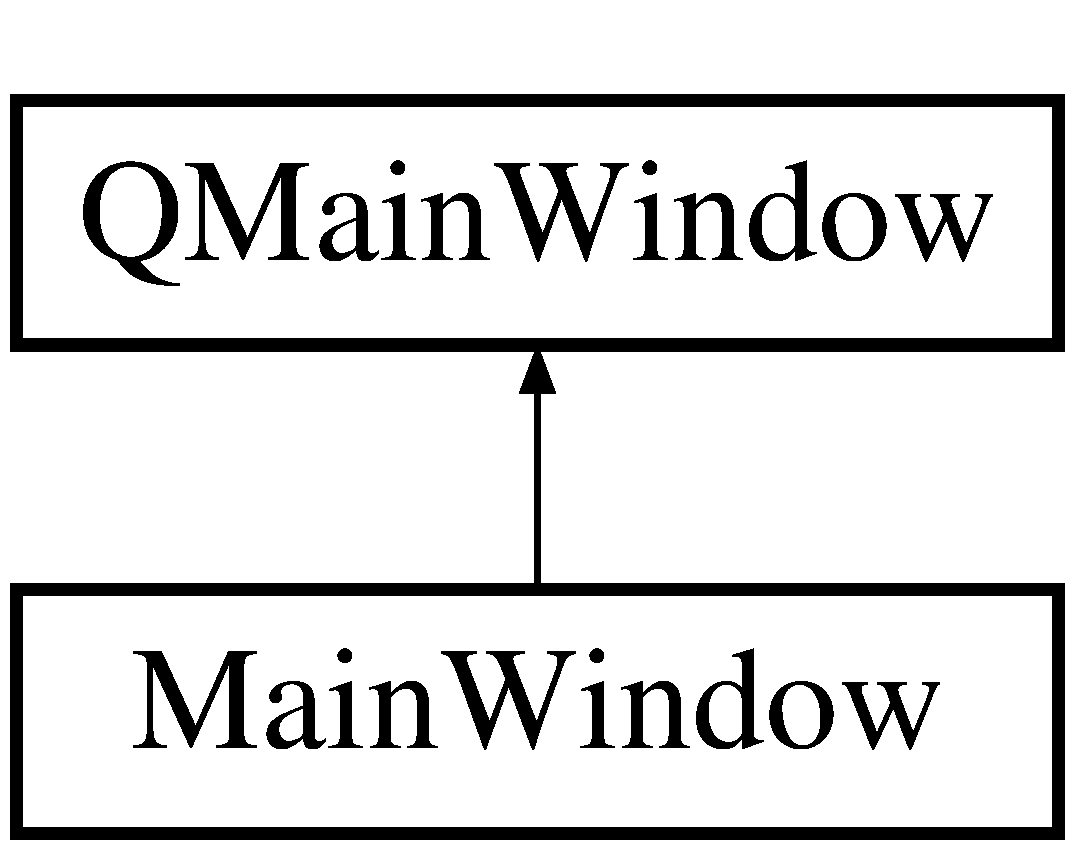
\includegraphics[height=2.000000cm]{class_main_window}
\end{center}
\end{figure}
\subsection*{Public Slots}
\begin{DoxyCompactItemize}
\item 
void \hyperlink{class_main_window_a69f73b93cc05c89a9ae1be0161105982}{new\+File} ()
\begin{DoxyCompactList}\small\item\em Actions and Menus. \end{DoxyCompactList}\item 
\hypertarget{class_main_window_a288b768c3c21a9171bdc56fe845ece8b}{}void {\bfseries open\+File} ()\label{class_main_window_a288b768c3c21a9171bdc56fe845ece8b}

\item 
\hypertarget{class_main_window_ad11e32151909b28e94538b146958d5a1}{}void {\bfseries close\+File} ()\label{class_main_window_ad11e32151909b28e94538b146958d5a1}

\item 
\hypertarget{class_main_window_aa90a352577dfc8ad0f7e6974f689b596}{}bool {\bfseries save\+File} (int index=-\/1)\label{class_main_window_aa90a352577dfc8ad0f7e6974f689b596}

\item 
\hypertarget{class_main_window_ace2d3f9e772a478c9e10467fc0707128}{}bool {\bfseries save\+As\+File} (int index=-\/1)\label{class_main_window_ace2d3f9e772a478c9e10467fc0707128}

\item 
\hypertarget{class_main_window_abbb16fb2d79a6a8c91695a1aad622383}{}void {\bfseries save\+Exe} ()\label{class_main_window_abbb16fb2d79a6a8c91695a1aad622383}

\item 
bool \hyperlink{class_main_window_a79cd135085ff501e05419fc7153c4e73}{close\+App} ()
\item 
void \hyperlink{class_main_window_a14b2be29dd502629c21f9ec1b0de5de4}{refresh\+Edit\+Menu} ()
\item 
\hypertarget{class_main_window_a117d0f9e30fade99d142818049a5a2b3}{}void {\bfseries change\+Current\+Saved\+State} (bool changed)\label{class_main_window_a117d0f9e30fade99d142818049a5a2b3}

\item 
\hypertarget{class_main_window_ab67a8002596d073eb1460fb06eeaff66}{}void \hyperlink{class_main_window_ab67a8002596d073eb1460fb06eeaff66}{open\+File} (Q\+String path)\label{class_main_window_ab67a8002596d073eb1460fb06eeaff66}

\begin{DoxyCompactList}\small\item\em Custom U\+N\+K\+N\+O\+W\+N. \end{DoxyCompactList}\item 
\hypertarget{class_main_window_a1308c0af5f2cb446322065b02fcbeaad}{}void {\bfseries other\+Instance\+Data\+Received} (Q\+Byte\+Array data)\label{class_main_window_a1308c0af5f2cb446322065b02fcbeaad}

\item 
void \hyperlink{class_main_window_a8584b048711a7a4fd68c042aeaf6d8e7}{build\+Program} (bool debug\+Mode=false)
\begin{DoxyCompactList}\small\item\em Build. \end{DoxyCompactList}\item 
\hypertarget{class_main_window_a82e7f9602ec1cf314ccd79dd4ef55c20}{}void {\bfseries run\+Program} ()\label{class_main_window_a82e7f9602ec1cf314ccd79dd4ef55c20}

\item 
\hypertarget{class_main_window_a6e289e447311bfd223d971e20abd9117}{}void {\bfseries run\+Exe\+Program} ()\label{class_main_window_a6e289e447311bfd223d971e20abd9117}

\item 
\hypertarget{class_main_window_a0e2d100b79aa592b649f0f9a9e35076f}{}void {\bfseries stop\+Program} ()\label{class_main_window_a0e2d100b79aa592b649f0f9a9e35076f}

\item 
\hypertarget{class_main_window_af0402980c9360426d2c996ecdc7374de}{}void {\bfseries test\+Stop\+Of\+Program} ()\label{class_main_window_af0402980c9360426d2c996ecdc7374de}

\item 
\hypertarget{class_main_window_a45faac26bdff89812539c065ef018a18}{}void {\bfseries set\+Program\+Builded\+Flag\+To\+False} ()\label{class_main_window_a45faac26bdff89812539c065ef018a18}

\item 
void \hyperlink{class_main_window_aeac9a226959ae44a5f8eedb73fbfaa94}{change\+Current\+Tab} (int index)
\item 
\hypertarget{class_main_window_a44a8bbdd1b143683bea71cfbad3a11b4}{}void {\bfseries print\+Log} (const Q\+String \&message, const Q\+Color \&color)\label{class_main_window_a44a8bbdd1b143683bea71cfbad3a11b4}

\item 
\hypertarget{class_main_window_a7b6f8754dcab273fe524bcaa30e67604}{}void {\bfseries print\+Log\+With\+Time} (const Q\+String \&message, const Q\+Color \&color)\label{class_main_window_a7b6f8754dcab273fe524bcaa30e67604}

\item 
\hypertarget{class_main_window_a52de98a5b987796cae5c2a1d5660037c}{}void {\bfseries start\+Count\+Program\+Time} ()\label{class_main_window_a52de98a5b987796cae5c2a1d5660037c}

\item 
void \hyperlink{class_main_window_ac1ebf6edc016999e6e55b58c2efc322e}{debug} ()
\begin{DoxyCompactList}\small\item\em Debug. \end{DoxyCompactList}\item 
void \hyperlink{class_main_window_a1ecd0f10a8b0acfaf63c1bb4f1b77cfb}{enable\+Debug\+Actions} ()
\item 
void \hyperlink{class_main_window_ad11440fb016244cd6f3fa947022ad713}{disable\+Debug\+Actions} (bool start=false)
\item 
\hypertarget{class_main_window_a3e9fb363847ac215097e42c5d2b12083}{}void {\bfseries debug\+Next} ()\label{class_main_window_a3e9fb363847ac215097e42c5d2b12083}

\item 
\hypertarget{class_main_window_a44cc0c28c3f5038f955a7e463497a9da}{}void {\bfseries debug\+Next\+Ni} ()\label{class_main_window_a44cc0c28c3f5038f955a7e463497a9da}

\item 
void \hyperlink{class_main_window_a0d8f20a9b47c566a76a96633188372fa}{debug\+Exit} ()
\item 
\hypertarget{class_main_window_aee811445332a4f7db279652ec332fe66}{}void {\bfseries debug\+Toggle\+Breakpoint} ()\label{class_main_window_aee811445332a4f7db279652ec332fe66}

\item 
\hypertarget{class_main_window_ac50abb82874b91085ceea8f565fd5f5a}{}void {\bfseries debug\+Show\+Registers} ()\label{class_main_window_ac50abb82874b91085ceea8f565fd5f5a}

\item 
void \hyperlink{class_main_window_af0e3a62c03cbe1723ba91d7cb21ec3c1}{debug\+Show\+Memory} ()
\item 
\hypertarget{class_main_window_a15b7242ca96db2dfaec976b3b6570aa6}{}void {\bfseries debug\+Run\+Command} (Q\+String command, bool print)\label{class_main_window_a15b7242ca96db2dfaec976b3b6570aa6}

\item 
\hypertarget{class_main_window_abcac2850930ae7f17bb5e01421630577}{}void {\bfseries save\+Watches} (\hyperlink{class_debug_table_widget}{Debug\+Table\+Widget} $\ast$table)\label{class_main_window_abcac2850930ae7f17bb5e01421630577}

\item 
\hypertarget{class_main_window_aa8e175e826ca88ed0edc86c4f58b2b3c}{}void {\bfseries set\+Show\+Registers\+To\+Unchecked} ()\label{class_main_window_aa8e175e826ca88ed0edc86c4f58b2b3c}

\item 
\hypertarget{class_main_window_aab119cfa893d26727179f37f4d93b9c3}{}void {\bfseries set\+Show\+Memory\+To\+Unchecked} ()\label{class_main_window_aab119cfa893d26727179f37f4d93b9c3}

\item 
\hypertarget{class_main_window_a94de085952cb2e1c2cabdf0589589bf7}{}void {\bfseries set\+Show\+Memory\+To\+Checked} (const \hyperlink{struct_ru_q_plain_text_edit_1_1_watch}{Ru\+Q\+Plain\+Text\+Edit\+::\+Watch} \&variable)\label{class_main_window_a94de085952cb2e1c2cabdf0589589bf7}

\item 
\hypertarget{class_main_window_a8208aa1ac575ce525eeb67962de39649}{}void {\bfseries show\+Any\+Command\+Widget} ()\label{class_main_window_a8208aa1ac575ce525eeb67962de39649}

\item 
\hypertarget{class_main_window_a4b549dce3792ad8e98c579b114dbf2d6}{}void {\bfseries close\+Any\+Command\+Widget} ()\label{class_main_window_a4b549dce3792ad8e98c579b114dbf2d6}

\item 
\hypertarget{class_main_window_a69a5788187930b71d8847316ea1ff400}{}void {\bfseries print\+Output} (Q\+String msg, int index=-\/1)\label{class_main_window_a69a5788187930b71d8847316ea1ff400}

\item 
\hypertarget{class_main_window_a7132389264d1fc06daf0f592ec390b63}{}void {\bfseries get\+Output} ()\label{class_main_window_a7132389264d1fc06daf0f592ec390b63}

\item 
\hypertarget{class_main_window_ac19a5fb34a804da9e7f970917843a680}{}void {\bfseries change\+Debug\+Action\+To\+Start} ()\label{class_main_window_ac19a5fb34a804da9e7f970917843a680}

\item 
\hypertarget{class_main_window_a069e1f54d0a804ca17cb8d4d78f093b0}{}void \hyperlink{class_main_window_a069e1f54d0a804ca17cb8d4d78f093b0}{find} ()\label{class_main_window_a069e1f54d0a804ca17cb8d4d78f093b0}

\begin{DoxyCompactList}\small\item\em Search. \end{DoxyCompactList}\item 
void \hyperlink{class_main_window_a56e46fe3769163f479d2a2b5eeb00b24}{find\+Next} (const Q\+String \&pattern, Qt\+::\+Case\+Sensitivity cs, bool all, bool replace, const Q\+String \&replace\+Text=0)
\item 
\hypertarget{class_main_window_a31b9332bdc8d48261497648c3faf2f91}{}void \hyperlink{class_main_window_a31b9332bdc8d48261497648c3faf2f91}{restore\+Prev\+Session} (bool not\+Notify=false)\label{class_main_window_a31b9332bdc8d48261497648c3faf2f91}

\begin{DoxyCompactList}\small\item\em Settings. \end{DoxyCompactList}\item 
void \hyperlink{class_main_window_a8e1c1ad87a68b27f19492549b9c4e773}{open\+Settings} ()
\item 
void \hyperlink{class_main_window_a31a22d06907f6f37fe53b3c1a78a27c4}{change\+Mode} (bool x86)
\item 
void \hyperlink{class_main_window_a117cad33e07cf5743d10390224ce9b20}{change\+Assembler} ()
\item 
\hypertarget{class_main_window_adc2c6917bad92be5f29b3f03bdcf3e2f}{}void {\bfseries change\+Start\+Text} ()\label{class_main_window_adc2c6917bad92be5f29b3f03bdcf3e2f}

\item 
void \hyperlink{class_main_window_abb30531afee763d0586ee6323fd332e2}{save\+Settings} ()
\item 
\hypertarget{class_main_window_a8d8a4882d5f3bfd14c1a9ad099cfed34}{}void {\bfseries exit\+Settings} ()\label{class_main_window_a8d8a4882d5f3bfd14c1a9ad099cfed34}

\item 
void \hyperlink{class_main_window_aee3cd5b22f4b0ec8e98b0a56d21e2ce4}{change\+Actions\+State} (int widget\+Index)
\item 
void \hyperlink{class_main_window_a03a1eafa1b4d6b1214767f408cbcf8c7}{reset\+All\+Settings} ()
\item 
\hypertarget{class_main_window_ad750f8cf1395c0383b01c97fe65cd515}{}void {\bfseries pick\+Color} (Q\+Widget $\ast$color\+Button, bool init=false)\label{class_main_window_ad750f8cf1395c0383b01c97fe65cd515}

\item 
\hypertarget{class_main_window_aec4ed4286d88e04c131cb882050c3fec}{}void {\bfseries change\+Highlighting\+Font} (Q\+Widget $\ast$box, bool init=false)\label{class_main_window_aec4ed4286d88e04c131cb882050c3fec}

\item 
\hypertarget{class_main_window_a588a4be0d3b05980878a5fa660996fc2}{}void {\bfseries change\+Highlighting\+Line\+Mode} (bool mode)\label{class_main_window_a588a4be0d3b05980878a5fa660996fc2}

\item 
\hypertarget{class_main_window_a6f43cd45a2b2ef207cabe97a8d8941e3}{}void {\bfseries recreate\+Highlighter} ()\label{class_main_window_a6f43cd45a2b2ef207cabe97a8d8941e3}

\item 
void \hyperlink{class_main_window_a4f00b18cd52e8ba0ef80cca56559cead}{recreate\+Assembler} (bool start=false)
\item 
void \hyperlink{class_main_window_ac778aed78fb6c50fecbdb174bad1b293}{init\+Assembler\+Settings} (bool first\+Opening)
\item 
\hypertarget{class_main_window_aeae98b66b64ca9c75095b6cbac38f4a2}{}void {\bfseries backup\+Settings} ()\label{class_main_window_aeae98b66b64ca9c75095b6cbac38f4a2}

\item 
\hypertarget{class_main_window_a555711d04fe9b975d620fbe79dbfdd87}{}void {\bfseries restore\+Settings\+And\+Exit} ()\label{class_main_window_a555711d04fe9b975d620fbe79dbfdd87}

\item 
void \hyperlink{class_main_window_a1f08865148ab71e63a82bff98cbd17c8}{print\+Masm\+Info} ()
\item 
\hypertarget{class_main_window_aa6eb8abce0304d5e6f84097dd433122b}{}void {\bfseries enable\+Or\+Disable\+Linking\+Edit} (int disable\+Linking\+Checkbox\+State)\label{class_main_window_aa6eb8abce0304d5e6f84097dd433122b}

\item 
bool \hyperlink{class_main_window_a2b789b53a039e5c900fccba3881cc16b}{delete\+Tab} (int index, bool save\+File\+Name=false)
\begin{DoxyCompactList}\small\item\em Closing. \end{DoxyCompactList}\item 
\hypertarget{class_main_window_a4f95292d59c2795f60e74b15b7b82af9}{}void {\bfseries close\+All\+Child\+Windows} ()\label{class_main_window_a4f95292d59c2795f60e74b15b7b82af9}

\item 
void \hyperlink{class_main_window_a4037900bbe42daa151e96ba5c96c8f62}{open\+Help} ()
\begin{DoxyCompactList}\small\item\em Help and About. \end{DoxyCompactList}\item 
\hypertarget{class_main_window_a06bcc3ac679ebab877652fc0d69744ea}{}void {\bfseries open\+About} ()\label{class_main_window_a06bcc3ac679ebab877652fc0d69744ea}

\end{DoxyCompactItemize}
\subsection*{Public Member Functions}
\begin{DoxyCompactItemize}
\item 
\hyperlink{class_main_window_affc2bb4c6ca84428e7121d8aac999164}{Main\+Window} (const Q\+String\+List \&args, Q\+Widget $\ast$parent=0)
\item 
\hyperlink{class_main_window_ae98d00a93bc118200eeef9f9bba1dba7}{$\sim$\+Main\+Window} ()
\item 
void \hyperlink{class_main_window_ad233094d8a8d6f41d81d845d1c4eb1ee}{init\+Ui} ()
\item 
\hypertarget{class_main_window_aa4907b0251d305659e403c62921ef331}{}void {\bfseries create\+Menus} ()\label{class_main_window_aa4907b0251d305659e403c62921ef331}

\item 
void \hyperlink{class_main_window_a62cd8712fb41a754298f6f60eead2cb0}{create\+Actions} ()
\item 
\hypertarget{class_main_window_a3a5152074fdfc6e75c6f86e55fcba28d}{}void {\bfseries create\+Buttons} ()\label{class_main_window_a3a5152074fdfc6e75c6f86e55fcba28d}

\item 
\hypertarget{class_main_window_acce4e32b95d3d5cb48470c053a1740c2}{}void {\bfseries create\+Tool\+Bars} ()\label{class_main_window_acce4e32b95d3d5cb48470c053a1740c2}

\item 
void \hyperlink{class_main_window_a49be45fc9b993fdc3afe55d4b6fa0650}{write\+Settings} ()
\item 
\hypertarget{class_main_window_a22a92325046401ede7a21e64728dd10b}{}void {\bfseries setup\+Editor} (int i)\label{class_main_window_a22a92325046401ede7a21e64728dd10b}

\item 
\hypertarget{class_main_window_a2ac2a11c4c75f5ee65f61e5c373581f6}{}bool {\bfseries ok\+To\+Continue} (int index=-\/1)\label{class_main_window_a2ac2a11c4c75f5ee65f61e5c373581f6}

\item 
void \hyperlink{class_main_window_a8f3241a37f8995ca0c20aeebdd2bfc24}{set\+Current\+Tab\+Name} (const Q\+String \&file\+Path, int index=-\/1)
\item 
\hypertarget{class_main_window_ad0252b4ac212cce0738ac8678309b2a0}{}bool {\bfseries remove\+Dir\+Recuresively} (const Q\+String \&dir\+Name)\label{class_main_window_ad0252b4ac212cce0738ac8678309b2a0}

\end{DoxyCompactItemize}
\subsection*{Protected Member Functions}
\begin{DoxyCompactItemize}
\item 
\hypertarget{class_main_window_a671bf73078069470c19965a3d948b6fa}{}void {\bfseries drag\+Enter\+Event} (Q\+Drag\+Enter\+Event $\ast$event)\label{class_main_window_a671bf73078069470c19965a3d948b6fa}

\item 
\hypertarget{class_main_window_ae7b97e68c51358f6f36be3c40b89c01c}{}void {\bfseries drop\+Event} (Q\+Drop\+Event $\ast$event)\label{class_main_window_ae7b97e68c51358f6f36be3c40b89c01c}

\end{DoxyCompactItemize}
\subsection*{Private Member Functions}
\begin{DoxyCompactItemize}
\item 
\hypertarget{class_main_window_a8a5bf36f9544ed3ec3a9eea9b7154564}{}void {\bfseries close\+Event} (Q\+Close\+Event $\ast$e)\label{class_main_window_a8a5bf36f9544ed3ec3a9eea9b7154564}

\end{DoxyCompactItemize}
\subsection*{Private Attributes}
\begin{DoxyCompactItemize}
\item 
\hypertarget{class_main_window_ab0d27cd951f836d48197c91349e02398}{}\hyperlink{class_get_started_widget}{Get\+Started\+Widget} $\ast$ {\bfseries get\+Started\+Widget}\label{class_main_window_ab0d27cd951f836d48197c91349e02398}

\item 
\hypertarget{class_main_window_ac789c1633000cdbf742f45f254ace59d}{}Q\+Stacked\+Widget $\ast$ {\bfseries main\+Widget}\label{class_main_window_ac789c1633000cdbf742f45f254ace59d}

\item 
\hypertarget{class_main_window_a392fb761a37795ee8081438c8c3493dd}{}Q\+Splitter $\ast$ {\bfseries splitter}\label{class_main_window_a392fb761a37795ee8081438c8c3493dd}

\item 
\hypertarget{class_main_window_abd2dd045cd4f4a425682e634515cee4a}{}Q\+V\+Box\+Layout $\ast$ {\bfseries work\+Layout}\label{class_main_window_abd2dd045cd4f4a425682e634515cee4a}

\item 
\hypertarget{class_main_window_aedb288ba31a9b42071fda2724afa8eb2}{}Q\+Widget $\ast$ {\bfseries work\+Widget}\label{class_main_window_aedb288ba31a9b42071fda2724afa8eb2}

\item 
\hypertarget{class_main_window_abbd98dca69e8cdc0aedf6330bc5a0960}{}\hyperlink{class_ru_q_text_edit}{Ru\+Q\+Text\+Edit} $\ast$ {\bfseries compiler\+Out}\label{class_main_window_abbd98dca69e8cdc0aedf6330bc5a0960}

\item 
\hypertarget{class_main_window_a7d5ec7879af0d224a6173a5565ea1ffd}{}Q\+Tab\+Widget $\ast$ {\bfseries tabs}\label{class_main_window_a7d5ec7879af0d224a6173a5565ea1ffd}

\item 
\hypertarget{class_main_window_a426da48f6e2f865b07a28533c07c4f7a}{}Q\+Menu $\ast$ \hyperlink{class_main_window_a426da48f6e2f865b07a28533c07c4f7a}{file\+Menu}\label{class_main_window_a426da48f6e2f865b07a28533c07c4f7a}

\begin{DoxyCompactList}\small\item\em Menus and Actions. \end{DoxyCompactList}\item 
\hypertarget{class_main_window_a5b05548b0849cd96a73ad5b38cc73bef}{}Q\+Menu $\ast$ {\bfseries edit\+Menu}\label{class_main_window_a5b05548b0849cd96a73ad5b38cc73bef}

\item 
\hypertarget{class_main_window_a2bfd2a3d19e9e750d25041306aa2923b}{}Q\+Menu $\ast$ {\bfseries debug\+Menu}\label{class_main_window_a2bfd2a3d19e9e750d25041306aa2923b}

\item 
\hypertarget{class_main_window_ab50ce8e7185bd0b16711a7a699dd907b}{}Q\+Menu $\ast$ {\bfseries build\+Menu}\label{class_main_window_ab50ce8e7185bd0b16711a7a699dd907b}

\item 
\hypertarget{class_main_window_a7e503c332056eb43ffa07fc664d34489}{}Q\+Menu $\ast$ {\bfseries settings\+Menu}\label{class_main_window_a7e503c332056eb43ffa07fc664d34489}

\item 
\hypertarget{class_main_window_a947c15e520bfea60338b2577f67146b8}{}Q\+Menu $\ast$ {\bfseries help\+Menu}\label{class_main_window_a947c15e520bfea60338b2577f67146b8}

\item 
\hypertarget{class_main_window_a5bcdb8d44feeff7d1bcb21f66a164255}{}Q\+Action $\ast$ {\bfseries new\+Action}\label{class_main_window_a5bcdb8d44feeff7d1bcb21f66a164255}

\item 
\hypertarget{class_main_window_ae988ea38c66b588f8f7e3f198aea46b0}{}Q\+Action $\ast$ {\bfseries open\+Action}\label{class_main_window_ae988ea38c66b588f8f7e3f198aea46b0}

\item 
\hypertarget{class_main_window_aa548b025a7f0179f05c928038c656fd7}{}Q\+Action $\ast$ {\bfseries close\+Action}\label{class_main_window_aa548b025a7f0179f05c928038c656fd7}

\item 
\hypertarget{class_main_window_a0ca0fd7bf38a67d5a0a985357566f396}{}Q\+Action $\ast$ {\bfseries save\+Action}\label{class_main_window_a0ca0fd7bf38a67d5a0a985357566f396}

\item 
\hypertarget{class_main_window_a6c23b775bc9e5820e87f9039ffdccf89}{}Q\+Action $\ast$ {\bfseries save\+As\+Action}\label{class_main_window_a6c23b775bc9e5820e87f9039ffdccf89}

\item 
\hypertarget{class_main_window_a0f48448ba8d20f4eb18430b5d9d8f54b}{}Q\+Action $\ast$ {\bfseries save\+Exe\+Action}\label{class_main_window_a0f48448ba8d20f4eb18430b5d9d8f54b}

\item 
\hypertarget{class_main_window_a480862e5bff02a85e6de35513eceff2c}{}Q\+Action $\ast$ {\bfseries exit\+Action}\label{class_main_window_a480862e5bff02a85e6de35513eceff2c}

\item 
\hypertarget{class_main_window_abd1e6457fc9a3441cc4e7046eb119a0f}{}Q\+Action $\ast$ {\bfseries find\+Action}\label{class_main_window_abd1e6457fc9a3441cc4e7046eb119a0f}

\item 
\hypertarget{class_main_window_a9c2a73fe97788e4d531747413e090e53}{}Q\+Action $\ast$ {\bfseries comment\+Action}\label{class_main_window_a9c2a73fe97788e4d531747413e090e53}

\item 
\hypertarget{class_main_window_a5dbf4af115805b62eb3e2aa072f737f8}{}Q\+Action $\ast$ {\bfseries uncomment\+Action}\label{class_main_window_a5dbf4af115805b62eb3e2aa072f737f8}

\item 
\hypertarget{class_main_window_a5781877445b8e6152ade56a71a4d8741}{}Q\+Action $\ast$ {\bfseries undo\+Action}\label{class_main_window_a5781877445b8e6152ade56a71a4d8741}

\item 
\hypertarget{class_main_window_a068e205ecfed3a2859e025e04f2f5f50}{}Q\+Action $\ast$ {\bfseries redo\+Action}\label{class_main_window_a068e205ecfed3a2859e025e04f2f5f50}

\item 
\hypertarget{class_main_window_a62adda2fa755a485b73d36ed37d9cbf6}{}Q\+Action $\ast$ {\bfseries cut\+Action}\label{class_main_window_a62adda2fa755a485b73d36ed37d9cbf6}

\item 
\hypertarget{class_main_window_a97c114ec68355261f327b83d5e19a5dc}{}Q\+Action $\ast$ {\bfseries copy\+Action}\label{class_main_window_a97c114ec68355261f327b83d5e19a5dc}

\item 
\hypertarget{class_main_window_a79595fa29fd4a746d701d6422cea5c86}{}Q\+Action $\ast$ {\bfseries paste\+Action}\label{class_main_window_a79595fa29fd4a746d701d6422cea5c86}

\item 
\hypertarget{class_main_window_acda4f1b59ac5e55f37e98e35bf5dc9b6}{}Q\+Action $\ast$ {\bfseries delete\+Action}\label{class_main_window_acda4f1b59ac5e55f37e98e35bf5dc9b6}

\item 
\hypertarget{class_main_window_a27a851d907e5cf54c2df75cdbb8a9003}{}Q\+Action $\ast$ {\bfseries select\+All\+Action}\label{class_main_window_a27a851d907e5cf54c2df75cdbb8a9003}

\item 
\hypertarget{class_main_window_acd9224aa5d181e9c6754cb71fc103e2f}{}Q\+Action $\ast$ {\bfseries put\+Tab\+Action}\label{class_main_window_acd9224aa5d181e9c6754cb71fc103e2f}

\item 
\hypertarget{class_main_window_a8f5db4cdc4dc7f610ace1b97f64f42fb}{}Q\+Action $\ast$ {\bfseries delete\+Tab\+Action}\label{class_main_window_a8f5db4cdc4dc7f610ace1b97f64f42fb}

\item 
\hypertarget{class_main_window_a29f530ec086e65c4a35eb28e68fd2236}{}Q\+Action $\ast$ {\bfseries build\+Action}\label{class_main_window_a29f530ec086e65c4a35eb28e68fd2236}

\item 
\hypertarget{class_main_window_a84ae1463c68554b9d2e3ff3fa2c30c25}{}Q\+Action $\ast$ {\bfseries run\+Action}\label{class_main_window_a84ae1463c68554b9d2e3ff3fa2c30c25}

\item 
\hypertarget{class_main_window_a9b4544dc6986833c366d47c5b83632bf}{}Q\+Action $\ast$ {\bfseries run\+Exe\+Action}\label{class_main_window_a9b4544dc6986833c366d47c5b83632bf}

\item 
\hypertarget{class_main_window_a9b1cc672dc054704f2dfbe47386793b5}{}Q\+Action $\ast$ {\bfseries stop\+Action}\label{class_main_window_a9b1cc672dc054704f2dfbe47386793b5}

\item 
\hypertarget{class_main_window_a4a8e530692fbabf29c34083616628bf9}{}Q\+Action $\ast$ {\bfseries debug\+Action}\label{class_main_window_a4a8e530692fbabf29c34083616628bf9}

\item 
\hypertarget{class_main_window_af618c0de06267e6b249bf5681dde4d45}{}Q\+Action $\ast$ {\bfseries debug\+Next\+Action}\label{class_main_window_af618c0de06267e6b249bf5681dde4d45}

\item 
\hypertarget{class_main_window_af10d588a7952b147e345945ef345cd1c}{}Q\+Action $\ast$ {\bfseries debug\+Next\+Ni\+Action}\label{class_main_window_af10d588a7952b147e345945ef345cd1c}

\item 
\hypertarget{class_main_window_a1526ae1c06e5cdace7bba5e3d17a0780}{}Q\+Action $\ast$ {\bfseries debug\+Toggle\+Breakpoint\+Action}\label{class_main_window_a1526ae1c06e5cdace7bba5e3d17a0780}

\item 
\hypertarget{class_main_window_abdf5fb2ab70cac959f1252548bb5df01}{}Q\+Action $\ast$ {\bfseries debug\+Show\+Registers\+Action}\label{class_main_window_abdf5fb2ab70cac959f1252548bb5df01}

\item 
\hypertarget{class_main_window_a2243efbdb97a03e431d2be5d6e6f870d}{}Q\+Action $\ast$ {\bfseries debug\+Show\+Memory\+Action}\label{class_main_window_a2243efbdb97a03e431d2be5d6e6f870d}

\item 
\hypertarget{class_main_window_a54cb5d217f90135a7c366d0b37331493}{}Q\+Action $\ast$ {\bfseries settings\+Action}\label{class_main_window_a54cb5d217f90135a7c366d0b37331493}

\item 
\hypertarget{class_main_window_add8f4264db92b536da73c849e14bd3c7}{}Q\+Action $\ast$ {\bfseries help\+Action}\label{class_main_window_add8f4264db92b536da73c849e14bd3c7}

\item 
\hypertarget{class_main_window_a4bc4ae131d91d1eece03c36fd0c2d3fa}{}Q\+Action $\ast$ {\bfseries about\+Action}\label{class_main_window_a4bc4ae131d91d1eece03c36fd0c2d3fa}

\item 
\hypertarget{class_main_window_a0a352c6d66b7a080fcf558874a7e51d4}{}Q\+Tool\+Bar $\ast$ \hyperlink{class_main_window_a0a352c6d66b7a080fcf558874a7e51d4}{file\+Tool\+Bar}\label{class_main_window_a0a352c6d66b7a080fcf558874a7e51d4}

\begin{DoxyCompactList}\small\item\em Toolbars. \end{DoxyCompactList}\item 
\hypertarget{class_main_window_a58acbb5fd760cdd016969a446abb83ca}{}Q\+Tool\+Bar $\ast$ {\bfseries edit\+Tool\+Bar}\label{class_main_window_a58acbb5fd760cdd016969a446abb83ca}

\item 
\hypertarget{class_main_window_aa6e68a631578e55575254dd029ae8145}{}Q\+Tool\+Bar $\ast$ {\bfseries build\+Tool\+Bar}\label{class_main_window_aa6e68a631578e55575254dd029ae8145}

\item 
\hypertarget{class_main_window_aa3194e1aeded7359e3b63db79ad73a71}{}Q\+Tool\+Bar $\ast$ {\bfseries debug\+Tool\+Bar}\label{class_main_window_aa3194e1aeded7359e3b63db79ad73a71}

\item 
\hypertarget{class_main_window_a087957e06d8d297f08221e508dfb326e}{}Q\+Process $\ast$ \hyperlink{class_main_window_a087957e06d8d297f08221e508dfb326e}{run\+Process}\label{class_main_window_a087957e06d8d297f08221e508dfb326e}

\begin{DoxyCompactList}\small\item\em Builder and debugger and all that concern to them. \end{DoxyCompactList}\item 
\hypertarget{class_main_window_a0781f612c0eee901117a42f3fa457683}{}\hyperlink{class_code_editor}{Code\+Editor} $\ast$ {\bfseries prev\+Code\+Editor}\label{class_main_window_a0781f612c0eee901117a42f3fa457683}

\item 
\hypertarget{class_main_window_a356578805ed1248a7f2807434cb0e5ee}{}Q\+Timer $\ast$ {\bfseries timer}\label{class_main_window_a356578805ed1248a7f2807434cb0e5ee}

\item 
\hypertarget{class_main_window_a532375be374a745d71c38659afc235ea}{}Q\+Time {\bfseries program\+Execution\+Time}\label{class_main_window_a532375be374a745d71c38659afc235ea}

\item 
\hypertarget{class_main_window_ade3454d10164efa50487db71a9e2fbd9}{}\hyperlink{class_debugger}{Debugger} $\ast$ {\bfseries debugger}\label{class_main_window_ade3454d10164efa50487db71a9e2fbd9}

\item 
\hypertarget{class_main_window_a393e70c554043c77c719373122d8fb31}{}bool {\bfseries program\+Is\+Builded}\label{class_main_window_a393e70c554043c77c719373122d8fb31}

\item 
\hypertarget{class_main_window_a765bcdb2472bb408de635274ba564f0b}{}Q\+Pointer$<$ \hyperlink{class_debug_table_widget}{Debug\+Table\+Widget} $>$ {\bfseries registers\+Window}\label{class_main_window_a765bcdb2472bb408de635274ba564f0b}

\item 
\hypertarget{class_main_window_ae29651235c4b3e55b1475e53c949d396}{}Q\+Dock\+Widget $\ast$ {\bfseries registers\+Dock}\label{class_main_window_ae29651235c4b3e55b1475e53c949d396}

\item 
\hypertarget{class_main_window_acfa36ea58edc35ba9c1ccf85d5eb4d4c}{}Q\+Pointer$<$ \hyperlink{class_debug_table_widget}{Debug\+Table\+Widget} $>$ {\bfseries memory\+Window}\label{class_main_window_acfa36ea58edc35ba9c1ccf85d5eb4d4c}

\item 
\hypertarget{class_main_window_a23eeda6f502e86e8186877f7c2b583eb}{}Q\+Dock\+Widget $\ast$ {\bfseries memory\+Dock}\label{class_main_window_a23eeda6f502e86e8186877f7c2b583eb}

\item 
\hypertarget{class_main_window_ad9e9b1792aeba47a7bb27f954dd5f95b}{}Q\+List$<$ \hyperlink{struct_ru_q_plain_text_edit_1_1_watch}{Ru\+Q\+Plain\+Text\+Edit\+::\+Watch} $>$ {\bfseries watches}\label{class_main_window_ad9e9b1792aeba47a7bb27f954dd5f95b}

\item 
\hypertarget{class_main_window_ab5c1ce4f3d677eaa17ada4ec162aec06}{}\hyperlink{class_debug_any_command_widget}{Debug\+Any\+Command\+Widget} $\ast$ {\bfseries debug\+Any\+Command\+Widget}\label{class_main_window_ab5c1ce4f3d677eaa17ada4ec162aec06}

\item 
\hypertarget{class_main_window_a5f3369b552ea5be75a14592ec73d2018}{}bool {\bfseries program\+Stopped}\label{class_main_window_a5f3369b552ea5be75a14592ec73d2018}

\item 
\hypertarget{class_main_window_ae71b480c580e95196e0541d091b29440}{}int {\bfseries output\+Index}\label{class_main_window_ae71b480c580e95196e0541d091b29440}

\item 
\hypertarget{class_main_window_adadee554364d68c67e145995bb0d6d88}{}\hyperlink{class_assembler}{Assembler} $\ast$ {\bfseries assembler}\label{class_main_window_adadee554364d68c67e145995bb0d6d88}

\item 
\hypertarget{class_main_window_a946e1a48859b30089dd5bfcfb2032ef9}{}bool {\bfseries debugger\+Was\+Started}\label{class_main_window_a946e1a48859b30089dd5bfcfb2032ef9}

\item 
\hypertarget{class_main_window_a101e50e1127fe118c8072fb654d2a6f4}{}Q\+String {\bfseries debug\+Key}\label{class_main_window_a101e50e1127fe118c8072fb654d2a6f4}

\item 
\hypertarget{class_main_window_ae653e799d7c4b702ad23f9a5f5b134e7}{}\hyperlink{class_highlighter}{Highlighter} $\ast$ \hyperlink{class_main_window_ae653e799d7c4b702ad23f9a5f5b134e7}{highlighter}\label{class_main_window_ae653e799d7c4b702ad23f9a5f5b134e7}

\begin{DoxyCompactList}\small\item\em Highlighters. \end{DoxyCompactList}\item 
\hypertarget{class_main_window_ac3ed715255e638544c915d3f5dcd0eed}{}\hyperlink{class_highlighter}{Highlighter} $\ast$ {\bfseries settings\+Highlighter}\label{class_main_window_ac3ed715255e638544c915d3f5dcd0eed}

\item 
\hypertarget{class_main_window_a940ef509338a6eb9a8fd88b744444528}{}Q\+Pointer$<$ \hyperlink{class_find_dialog}{Find\+Dialog} $>$ \hyperlink{class_main_window_a940ef509338a6eb9a8fd88b744444528}{find\+Dialog}\label{class_main_window_a940ef509338a6eb9a8fd88b744444528}

\begin{DoxyCompactList}\small\item\em Search. \end{DoxyCompactList}\item 
\hypertarget{class_main_window_a4675f0ccc7830548cdb633bd7d203311}{}Qt\+::\+Case\+Sensitivity {\bfseries prev\+Cs}\label{class_main_window_a4675f0ccc7830548cdb633bd7d203311}

\item 
\hypertarget{class_main_window_aa26c478fd01dfb62f25cea707f46828f}{}Q\+Pointer$<$ Q\+Widget $>$ \hyperlink{class_main_window_aa26c478fd01dfb62f25cea707f46828f}{settings\+Window}\label{class_main_window_aa26c478fd01dfb62f25cea707f46828f}

\begin{DoxyCompactList}\small\item\em Settings and Help. \end{DoxyCompactList}\item 
\hypertarget{class_main_window_addb2c09eaa063aafb1a199f0ccdfe58a}{}Ui\+::\+Settings\+Window {\bfseries settings\+Ui}\label{class_main_window_addb2c09eaa063aafb1a199f0ccdfe58a}

\item 
\hypertarget{class_main_window_a4c0f162aea1aef936ce3cd6568d744d9}{}Q\+String {\bfseries start\+Text}\label{class_main_window_a4c0f162aea1aef936ce3cd6568d744d9}

\item 
\hypertarget{class_main_window_a017ec0eacfb8f3a4bc7656e75adb3610}{}\hyperlink{class_code_editor}{Code\+Editor} $\ast$ {\bfseries settings\+Start\+Text\+Editor}\label{class_main_window_a017ec0eacfb8f3a4bc7656e75adb3610}

\item 
\hypertarget{class_main_window_a314ff864f3e545e033898d3d4f136d52}{}Q\+String \hyperlink{class_main_window_a314ff864f3e545e033898d3d4f136d52}{save\+Open\+Directory}\label{class_main_window_a314ff864f3e545e033898d3d4f136d52}

\begin{DoxyCompactList}\small\item\em save and open \end{DoxyCompactList}\item 
\hypertarget{class_main_window_a0198da4de1adda89a1418a87168f66c6}{}Q\+Pointer$<$ Q\+Text\+Browser $>$ {\bfseries help}\label{class_main_window_a0198da4de1adda89a1418a87168f66c6}

\item 
\hypertarget{class_main_window_a4fd9ec8df088f03433cb7937adadcc34}{}Q\+Signal\+Mapper $\ast$ {\bfseries color\+Signal\+Mapper}\label{class_main_window_a4fd9ec8df088f03433cb7937adadcc34}

\item 
\hypertarget{class_main_window_a0ede638df0e7f1ed317c83ebdf790c7e}{}Q\+Signal\+Mapper $\ast$ {\bfseries fonts\+Signal\+Mapper}\label{class_main_window_a0ede638df0e7f1ed317c83ebdf790c7e}

\item 
\hypertarget{class_main_window_afdd7b3115692de072db9504d38449ae9}{}Q\+List$<$ Q\+Push\+Button $\ast$ $>$ {\bfseries color\+Buttons}\label{class_main_window_afdd7b3115692de072db9504d38449ae9}

\item 
\hypertarget{class_main_window_aabb23f3b2db87626123838f7705f3f15}{}Q\+List$<$ Q\+Color $>$ \hyperlink{class_main_window_aabb23f3b2db87626123838f7705f3f15}{default\+Colors}\label{class_main_window_aabb23f3b2db87626123838f7705f3f15}

\begin{DoxyCompactList}\small\item\em According to color\+Buttons. \end{DoxyCompactList}\item 
\hypertarget{class_main_window_a3b3d9502ca6548f19f81b3e9921e8e1f}{}Q\+Map$<$ Q\+String, Q\+Color $>$ {\bfseries colors\+Map}\label{class_main_window_a3b3d9502ca6548f19f81b3e9921e8e1f}

\item 
\hypertarget{class_main_window_a41a492577e8a6dd51b9b9a78a236c6c0}{}Q\+List$<$ Q\+Check\+Box $\ast$ $>$ {\bfseries font\+Check\+Boxes}\label{class_main_window_a41a492577e8a6dd51b9b9a78a236c6c0}

\item 
\hypertarget{class_main_window_a87b5b9562fe91ee19249f5a0d7617ce0}{}Q\+Settings {\bfseries settings}\label{class_main_window_a87b5b9562fe91ee19249f5a0d7617ce0}

\item 
\hypertarget{class_main_window_aa9410fd13b6463955726d700de837323}{}Q\+String {\bfseries backup\+Assembler}\label{class_main_window_aa9410fd13b6463955726d700de837323}

\item 
\hypertarget{class_main_window_a6ebfecf17b4a7b7931daa5198fbc0b44}{}Q\+String {\bfseries backup\+Mode}\label{class_main_window_a6ebfecf17b4a7b7931daa5198fbc0b44}

\item 
\hypertarget{class_main_window_a1af0453c231c87ff14067103b3121803}{}Q\+String {\bfseries backup\+Assembler\+Options}\label{class_main_window_a1af0453c231c87ff14067103b3121803}

\item 
\hypertarget{class_main_window_a1fe62872a358a8f6f20e96c02a9be62f}{}Q\+String {\bfseries backup\+Linker\+Options}\label{class_main_window_a1fe62872a358a8f6f20e96c02a9be62f}

\item 
\hypertarget{class_main_window_a11c38f51d33a2369f1bd444be72975af}{}bool {\bfseries backup\+Disable\+Linking}\label{class_main_window_a11c38f51d33a2369f1bd444be72975af}

\item 
\hypertarget{class_main_window_a44be17fe698b7a47c0d118379075c8e9}{}Q\+String {\bfseries backup\+Assembler\+Path}\label{class_main_window_a44be17fe698b7a47c0d118379075c8e9}

\item 
\hypertarget{class_main_window_a36891330292ae023d8de31113a555b63}{}Q\+String {\bfseries backup\+Start\+Text}\label{class_main_window_a36891330292ae023d8de31113a555b63}

\item 
\hypertarget{class_main_window_ad28f0fe6e6dc8caf75173b19db1972c4}{}Q\+String {\bfseries backup\+Linker\+Path}\label{class_main_window_ad28f0fe6e6dc8caf75173b19db1972c4}

\item 
\hypertarget{class_main_window_a4b71407a32d640de521b24eed1c8d672}{}bool \hyperlink{class_main_window_a4b71407a32d640de521b24eed1c8d672}{close\+From\+Close\+All}\label{class_main_window_a4b71407a32d640de521b24eed1c8d672}

\begin{DoxyCompactList}\small\item\em About close. \end{DoxyCompactList}\end{DoxyCompactItemize}


\subsection{Detailed Description}
The \hyperlink{class_main_window}{Main\+Window} class defines the actions and behavior of the main user interface. 

Longer explanation here 

\subsection{Constructor \& Destructor Documentation}
\hypertarget{class_main_window_affc2bb4c6ca84428e7121d8aac999164}{}\index{Main\+Window@{Main\+Window}!Main\+Window@{Main\+Window}}
\index{Main\+Window@{Main\+Window}!Main\+Window@{Main\+Window}}
\subsubsection[{Main\+Window}]{\setlength{\rightskip}{0pt plus 5cm}Main\+Window\+::\+Main\+Window (
\begin{DoxyParamCaption}
\item[{const Q\+String\+List \&}]{args, }
\item[{Q\+Widget $\ast$}]{parent = {\ttfamily 0}}
\end{DoxyParamCaption}
)}\label{class_main_window_affc2bb4c6ca84428e7121d8aac999164}
Set save and open directory

Initial variables

Initialize assembler

Set code field start text

Restore log splitter state

Open documents from command line \hypertarget{class_main_window_ae98d00a93bc118200eeef9f9bba1dba7}{}\index{Main\+Window@{Main\+Window}!````~Main\+Window@{$\sim$\+Main\+Window}}
\index{````~Main\+Window@{$\sim$\+Main\+Window}!Main\+Window@{Main\+Window}}
\subsubsection[{$\sim$\+Main\+Window}]{\setlength{\rightskip}{0pt plus 5cm}Main\+Window\+::$\sim$\+Main\+Window (
\begin{DoxyParamCaption}
{}
\end{DoxyParamCaption}
)}\label{class_main_window_ae98d00a93bc118200eeef9f9bba1dba7}
Delete all temporary files 

\subsection{Member Function Documentation}
\hypertarget{class_main_window_a8584b048711a7a4fd68c042aeaf6d8e7}{}\index{Main\+Window@{Main\+Window}!build\+Program@{build\+Program}}
\index{build\+Program@{build\+Program}!Main\+Window@{Main\+Window}}
\subsubsection[{build\+Program}]{\setlength{\rightskip}{0pt plus 5cm}void Main\+Window\+::build\+Program (
\begin{DoxyParamCaption}
\item[{bool}]{debug\+Mode = {\ttfamily false}}
\end{DoxyParamCaption}
)\hspace{0.3cm}{\ttfamily [slot]}}\label{class_main_window_a8584b048711a7a4fd68c042aeaf6d8e7}


Build. 

Save input to file

\hyperlink{class_assembler}{Assembler}

G\+C\+C

macro.\+c compilation/copying

macro.\+c compilation

Final linking

Print errors

Q\+Message\+Box\+::critical(0, tr(\char`\"{}\+Warning!\char`\"{}), tr(\char`\"{}\+Errors have occurred in the build!\char`\"{}));

print warnings \hypertarget{class_main_window_aee3cd5b22f4b0ec8e98b0a56d21e2ce4}{}\index{Main\+Window@{Main\+Window}!change\+Actions\+State@{change\+Actions\+State}}
\index{change\+Actions\+State@{change\+Actions\+State}!Main\+Window@{Main\+Window}}
\subsubsection[{change\+Actions\+State}]{\setlength{\rightskip}{0pt plus 5cm}void Main\+Window\+::change\+Actions\+State (
\begin{DoxyParamCaption}
\item[{int}]{widget\+Index}
\end{DoxyParamCaption}
)\hspace{0.3cm}{\ttfamily [slot]}}\label{class_main_window_aee3cd5b22f4b0ec8e98b0a56d21e2ce4}
Get started window \hypertarget{class_main_window_a117cad33e07cf5743d10390224ce9b20}{}\index{Main\+Window@{Main\+Window}!change\+Assembler@{change\+Assembler}}
\index{change\+Assembler@{change\+Assembler}!Main\+Window@{Main\+Window}}
\subsubsection[{change\+Assembler}]{\setlength{\rightskip}{0pt plus 5cm}void Main\+Window\+::change\+Assembler (
\begin{DoxyParamCaption}
{}
\end{DoxyParamCaption}
)\hspace{0.3cm}{\ttfamily [slot]}}\label{class_main_window_a117cad33e07cf5743d10390224ce9b20}
\hyperlink{class_assembler}{Assembler} Dependent Options Begin \hypertarget{class_main_window_aeac9a226959ae44a5f8eedb73fbfaa94}{}\index{Main\+Window@{Main\+Window}!change\+Current\+Tab@{change\+Current\+Tab}}
\index{change\+Current\+Tab@{change\+Current\+Tab}!Main\+Window@{Main\+Window}}
\subsubsection[{change\+Current\+Tab}]{\setlength{\rightskip}{0pt plus 5cm}void Main\+Window\+::change\+Current\+Tab (
\begin{DoxyParamCaption}
\item[{int}]{index}
\end{DoxyParamCaption}
)\hspace{0.3cm}{\ttfamily [slot]}}\label{class_main_window_aeac9a226959ae44a5f8eedb73fbfaa94}
Set highlighter \hypertarget{class_main_window_a31a22d06907f6f37fe53b3c1a78a27c4}{}\index{Main\+Window@{Main\+Window}!change\+Mode@{change\+Mode}}
\index{change\+Mode@{change\+Mode}!Main\+Window@{Main\+Window}}
\subsubsection[{change\+Mode}]{\setlength{\rightskip}{0pt plus 5cm}void Main\+Window\+::change\+Mode (
\begin{DoxyParamCaption}
\item[{bool}]{x86}
\end{DoxyParamCaption}
)\hspace{0.3cm}{\ttfamily [slot]}}\label{class_main_window_a31a22d06907f6f37fe53b3c1a78a27c4}
\hyperlink{class_assembler}{Assembler} Dependent Options End \hypertarget{class_main_window_a79cd135085ff501e05419fc7153c4e73}{}\index{Main\+Window@{Main\+Window}!close\+App@{close\+App}}
\index{close\+App@{close\+App}!Main\+Window@{Main\+Window}}
\subsubsection[{close\+App}]{\setlength{\rightskip}{0pt plus 5cm}bool Main\+Window\+::close\+App (
\begin{DoxyParamCaption}
{}
\end{DoxyParamCaption}
)\hspace{0.3cm}{\ttfamily [slot]}}\label{class_main_window_a79cd135085ff501e05419fc7153c4e73}
Consider all tabs

Left only saved tabs \hypertarget{class_main_window_a62cd8712fb41a754298f6f60eead2cb0}{}\index{Main\+Window@{Main\+Window}!create\+Actions@{create\+Actions}}
\index{create\+Actions@{create\+Actions}!Main\+Window@{Main\+Window}}
\subsubsection[{create\+Actions}]{\setlength{\rightskip}{0pt plus 5cm}void Main\+Window\+::create\+Actions (
\begin{DoxyParamCaption}
{}
\end{DoxyParamCaption}
)}\label{class_main_window_a62cd8712fb41a754298f6f60eead2cb0}
Action in edit menu connects in refresh\+Edit\+Menu function!

Enable in run\+Program(), disable in stop

Disable some actions if get started widget opened \hypertarget{class_main_window_ac1ebf6edc016999e6e55b58c2efc322e}{}\index{Main\+Window@{Main\+Window}!debug@{debug}}
\index{debug@{debug}!Main\+Window@{Main\+Window}}
\subsubsection[{debug}]{\setlength{\rightskip}{0pt plus 5cm}void Main\+Window\+::debug (
\begin{DoxyParamCaption}
{}
\end{DoxyParamCaption}
)\hspace{0.3cm}{\ttfamily [slot]}}\label{class_main_window_ac1ebf6edc016999e6e55b58c2efc322e}


Debug. 

Start debugger if true \hypertarget{class_main_window_a0d8f20a9b47c566a76a96633188372fa}{}\index{Main\+Window@{Main\+Window}!debug\+Exit@{debug\+Exit}}
\index{debug\+Exit@{debug\+Exit}!Main\+Window@{Main\+Window}}
\subsubsection[{debug\+Exit}]{\setlength{\rightskip}{0pt plus 5cm}void Main\+Window\+::debug\+Exit (
\begin{DoxyParamCaption}
{}
\end{DoxyParamCaption}
)\hspace{0.3cm}{\ttfamily [slot]}}\label{class_main_window_a0d8f20a9b47c566a76a96633188372fa}
Many actions performed here -\/ deleting of highlighting too \hypertarget{class_main_window_af0e3a62c03cbe1723ba91d7cb21ec3c1}{}\index{Main\+Window@{Main\+Window}!debug\+Show\+Memory@{debug\+Show\+Memory}}
\index{debug\+Show\+Memory@{debug\+Show\+Memory}!Main\+Window@{Main\+Window}}
\subsubsection[{debug\+Show\+Memory}]{\setlength{\rightskip}{0pt plus 5cm}void Main\+Window\+::debug\+Show\+Memory (
\begin{DoxyParamCaption}
{}
\end{DoxyParamCaption}
)\hspace{0.3cm}{\ttfamily [slot]}}\label{class_main_window_af0e3a62c03cbe1723ba91d7cb21ec3c1}
Create table

Fill table

If true, watch as variable

Watch as random address \hypertarget{class_main_window_a2b789b53a039e5c900fccba3881cc16b}{}\index{Main\+Window@{Main\+Window}!delete\+Tab@{delete\+Tab}}
\index{delete\+Tab@{delete\+Tab}!Main\+Window@{Main\+Window}}
\subsubsection[{delete\+Tab}]{\setlength{\rightskip}{0pt plus 5cm}bool Main\+Window\+::delete\+Tab (
\begin{DoxyParamCaption}
\item[{int}]{index, }
\item[{bool}]{save\+File\+Name = {\ttfamily false}}
\end{DoxyParamCaption}
)\hspace{0.3cm}{\ttfamily [slot]}}\label{class_main_window_a2b789b53a039e5c900fccba3881cc16b}


Closing. 

Get started

If tab did not delete \hypertarget{class_main_window_ad11440fb016244cd6f3fa947022ad713}{}\index{Main\+Window@{Main\+Window}!disable\+Debug\+Actions@{disable\+Debug\+Actions}}
\index{disable\+Debug\+Actions@{disable\+Debug\+Actions}!Main\+Window@{Main\+Window}}
\subsubsection[{disable\+Debug\+Actions}]{\setlength{\rightskip}{0pt plus 5cm}void Main\+Window\+::disable\+Debug\+Actions (
\begin{DoxyParamCaption}
\item[{bool}]{start = {\ttfamily false}}
\end{DoxyParamCaption}
)\hspace{0.3cm}{\ttfamily [slot]}}\label{class_main_window_ad11440fb016244cd6f3fa947022ad713}
Change stop\+Action

Enable run and build \hypertarget{class_main_window_a1ecd0f10a8b0acfaf63c1bb4f1b77cfb}{}\index{Main\+Window@{Main\+Window}!enable\+Debug\+Actions@{enable\+Debug\+Actions}}
\index{enable\+Debug\+Actions@{enable\+Debug\+Actions}!Main\+Window@{Main\+Window}}
\subsubsection[{enable\+Debug\+Actions}]{\setlength{\rightskip}{0pt plus 5cm}void Main\+Window\+::enable\+Debug\+Actions (
\begin{DoxyParamCaption}
{}
\end{DoxyParamCaption}
)\hspace{0.3cm}{\ttfamily [slot]}}\label{class_main_window_a1ecd0f10a8b0acfaf63c1bb4f1b77cfb}
Set all user's breakpoints

Enable all actions

Change stop\+Action

Block run and build

Restore windows \hypertarget{class_main_window_a56e46fe3769163f479d2a2b5eeb00b24}{}\index{Main\+Window@{Main\+Window}!find\+Next@{find\+Next}}
\index{find\+Next@{find\+Next}!Main\+Window@{Main\+Window}}
\subsubsection[{find\+Next}]{\setlength{\rightskip}{0pt plus 5cm}void Main\+Window\+::find\+Next (
\begin{DoxyParamCaption}
\item[{const Q\+String \&}]{pattern, }
\item[{Qt\+::\+Case\+Sensitivity}]{cs, }
\item[{bool}]{all, }
\item[{bool}]{replace, }
\item[{const Q\+String \&}]{replace\+Text = {\ttfamily 0}}
\end{DoxyParamCaption}
)\hspace{0.3cm}{\ttfamily [slot]}}\label{class_main_window_a56e46fe3769163f479d2a2b5eeb00b24}
Clear all highlights and disable highlighting of current line

Restore highlight

Replace mode

Highlight all

Find next only

if documents differ, cursor is ignored in Q\+Text\+Document\+::find()

Continue from start \hypertarget{class_main_window_ac778aed78fb6c50fecbdb174bad1b293}{}\index{Main\+Window@{Main\+Window}!init\+Assembler\+Settings@{init\+Assembler\+Settings}}
\index{init\+Assembler\+Settings@{init\+Assembler\+Settings}!Main\+Window@{Main\+Window}}
\subsubsection[{init\+Assembler\+Settings}]{\setlength{\rightskip}{0pt plus 5cm}void Main\+Window\+::init\+Assembler\+Settings (
\begin{DoxyParamCaption}
\item[{bool}]{first\+Opening}
\end{DoxyParamCaption}
)\hspace{0.3cm}{\ttfamily [slot]}}\label{class_main_window_ac778aed78fb6c50fecbdb174bad1b293}
\hyperlink{class_assembler}{Assembler} Dependent Options Begin

\hyperlink{class_assembler}{Assembler} Dependent Options End

Start text editor

Build options

Mode

\hyperlink{class_assembler}{Assembler} Dependent Options Begin\hypertarget{class_main_window_ad233094d8a8d6f41d81d845d1c4eb1ee}{}\index{Main\+Window@{Main\+Window}!init\+Ui@{init\+Ui}}
\index{init\+Ui@{init\+Ui}!Main\+Window@{Main\+Window}}
\subsubsection[{init\+Ui}]{\setlength{\rightskip}{0pt plus 5cm}void Main\+Window\+::init\+Ui (
\begin{DoxyParamCaption}
{}
\end{DoxyParamCaption}
)}\label{class_main_window_ad233094d8a8d6f41d81d845d1c4eb1ee}
Resize

Set maximized

Get Started window

Create form

Stacked widget

Create highlighter

Create tabs

Create compiler field

Create gdb command widget

Add widgets on splitter

Restore previous session if it in settings \hypertarget{class_main_window_a69f73b93cc05c89a9ae1be0161105982}{}\index{Main\+Window@{Main\+Window}!new\+File@{new\+File}}
\index{new\+File@{new\+File}!Main\+Window@{Main\+Window}}
\subsubsection[{new\+File}]{\setlength{\rightskip}{0pt plus 5cm}void Main\+Window\+::new\+File (
\begin{DoxyParamCaption}
{}
\end{DoxyParamCaption}
)\hspace{0.3cm}{\ttfamily [slot]}}\label{class_main_window_a69f73b93cc05c89a9ae1be0161105982}


Actions and Menus. 

Tabs \hypertarget{class_main_window_a4037900bbe42daa151e96ba5c96c8f62}{}\index{Main\+Window@{Main\+Window}!open\+Help@{open\+Help}}
\index{open\+Help@{open\+Help}!Main\+Window@{Main\+Window}}
\subsubsection[{open\+Help}]{\setlength{\rightskip}{0pt plus 5cm}void Main\+Window\+::open\+Help (
\begin{DoxyParamCaption}
{}
\end{DoxyParamCaption}
)\hspace{0.3cm}{\ttfamily [slot]}}\label{class_main_window_a4037900bbe42daa151e96ba5c96c8f62}


Help and About. 

language 0=Russian

English language \hypertarget{class_main_window_a8e1c1ad87a68b27f19492549b9c4e773}{}\index{Main\+Window@{Main\+Window}!open\+Settings@{open\+Settings}}
\index{open\+Settings@{open\+Settings}!Main\+Window@{Main\+Window}}
\subsubsection[{open\+Settings}]{\setlength{\rightskip}{0pt plus 5cm}void Main\+Window\+::open\+Settings (
\begin{DoxyParamCaption}
{}
\end{DoxyParamCaption}
)\hspace{0.3cm}{\ttfamily [slot]}}\label{class_main_window_a8e1c1ad87a68b27f19492549b9c4e773}
Initialize

Colors

Foreground

Background

Common

According to color\+Buttons

Add color to associative array

Fonts

Bold

Italic

Add font to associative array

Set settings Common

Colors

Fonts \hypertarget{class_main_window_a1f08865148ab71e63a82bff98cbd17c8}{}\index{Main\+Window@{Main\+Window}!print\+Masm\+Info@{print\+Masm\+Info}}
\index{print\+Masm\+Info@{print\+Masm\+Info}!Main\+Window@{Main\+Window}}
\subsubsection[{print\+Masm\+Info}]{\setlength{\rightskip}{0pt plus 5cm}void Main\+Window\+::print\+Masm\+Info (
\begin{DoxyParamCaption}
{}
\end{DoxyParamCaption}
)\hspace{0.3cm}{\ttfamily [slot]}}\label{class_main_window_a1f08865148ab71e63a82bff98cbd17c8}
\hyperlink{class_assembler}{Assembler} Dependent Options End \hypertarget{class_main_window_a4f00b18cd52e8ba0ef80cca56559cead}{}\index{Main\+Window@{Main\+Window}!recreate\+Assembler@{recreate\+Assembler}}
\index{recreate\+Assembler@{recreate\+Assembler}!Main\+Window@{Main\+Window}}
\subsubsection[{recreate\+Assembler}]{\setlength{\rightskip}{0pt plus 5cm}void Main\+Window\+::recreate\+Assembler (
\begin{DoxyParamCaption}
\item[{bool}]{start = {\ttfamily false}}
\end{DoxyParamCaption}
)\hspace{0.3cm}{\ttfamily [slot]}}\label{class_main_window_a4f00b18cd52e8ba0ef80cca56559cead}
\hyperlink{class_assembler}{Assembler} Dependent Options Begin

\hyperlink{class_assembler}{Assembler} Dependent Options End\hypertarget{class_main_window_a14b2be29dd502629c21f9ec1b0de5de4}{}\index{Main\+Window@{Main\+Window}!refresh\+Edit\+Menu@{refresh\+Edit\+Menu}}
\index{refresh\+Edit\+Menu@{refresh\+Edit\+Menu}!Main\+Window@{Main\+Window}}
\subsubsection[{refresh\+Edit\+Menu}]{\setlength{\rightskip}{0pt plus 5cm}void Main\+Window\+::refresh\+Edit\+Menu (
\begin{DoxyParamCaption}
{}
\end{DoxyParamCaption}
)\hspace{0.3cm}{\ttfamily [slot]}}\label{class_main_window_a14b2be29dd502629c21f9ec1b0de5de4}
Disconnect from previous

Connect to current \hypertarget{class_main_window_a03a1eafa1b4d6b1214767f408cbcf8c7}{}\index{Main\+Window@{Main\+Window}!reset\+All\+Settings@{reset\+All\+Settings}}
\index{reset\+All\+Settings@{reset\+All\+Settings}!Main\+Window@{Main\+Window}}
\subsubsection[{reset\+All\+Settings}]{\setlength{\rightskip}{0pt plus 5cm}void Main\+Window\+::reset\+All\+Settings (
\begin{DoxyParamCaption}
{}
\end{DoxyParamCaption}
)\hspace{0.3cm}{\ttfamily [slot]}}\label{class_main_window_a03a1eafa1b4d6b1214767f408cbcf8c7}
Ask before execution

Remove previous \hypertarget{class_main_window_abb30531afee763d0586ee6323fd332e2}{}\index{Main\+Window@{Main\+Window}!save\+Settings@{save\+Settings}}
\index{save\+Settings@{save\+Settings}!Main\+Window@{Main\+Window}}
\subsubsection[{save\+Settings}]{\setlength{\rightskip}{0pt plus 5cm}void Main\+Window\+::save\+Settings (
\begin{DoxyParamCaption}
{}
\end{DoxyParamCaption}
)\hspace{0.3cm}{\ttfamily [slot]}}\label{class_main_window_abb30531afee763d0586ee6323fd332e2}
Change fonts \hypertarget{class_main_window_a8f3241a37f8995ca0c20aeebdd2bfc24}{}\index{Main\+Window@{Main\+Window}!set\+Current\+Tab\+Name@{set\+Current\+Tab\+Name}}
\index{set\+Current\+Tab\+Name@{set\+Current\+Tab\+Name}!Main\+Window@{Main\+Window}}
\subsubsection[{set\+Current\+Tab\+Name}]{\setlength{\rightskip}{0pt plus 5cm}void Main\+Window\+::set\+Current\+Tab\+Name (
\begin{DoxyParamCaption}
\item[{const Q\+String \&}]{file\+Path, }
\item[{int}]{index = {\ttfamily -\/1}}
\end{DoxyParamCaption}
)}\label{class_main_window_a8f3241a37f8995ca0c20aeebdd2bfc24}
Taking name of file (without path) \hypertarget{class_main_window_a49be45fc9b993fdc3afe55d4b6fa0650}{}\index{Main\+Window@{Main\+Window}!write\+Settings@{write\+Settings}}
\index{write\+Settings@{write\+Settings}!Main\+Window@{Main\+Window}}
\subsubsection[{write\+Settings}]{\setlength{\rightskip}{0pt plus 5cm}void Main\+Window\+::write\+Settings (
\begin{DoxyParamCaption}
{}
\end{DoxyParamCaption}
)}\label{class_main_window_a49be45fc9b993fdc3afe55d4b6fa0650}
G\+U\+I

Opened tabs

Remove previous

Create current

Save and open directory

Splitters state 

The documentation for this class was generated from the following files\+:\begin{DoxyCompactItemize}
\item 
\hyperlink{mainwindow_8h}{mainwindow.\+h}\item 
\hyperlink{mainwindow_8cpp}{mainwindow.\+cpp}\end{DoxyCompactItemize}

\hypertarget{class_m_a_s_m}{}\section{M\+A\+S\+M Class Reference}
\label{class_m_a_s_m}\index{M\+A\+S\+M@{M\+A\+S\+M}}


This class defines the behavior for the \hyperlink{class_m_a_s_m}{M\+A\+S\+M} assembler.  




{\ttfamily \#include $<$masm.\+h$>$}

Inheritance diagram for M\+A\+S\+M\+:\begin{figure}[H]
\begin{center}
\leavevmode
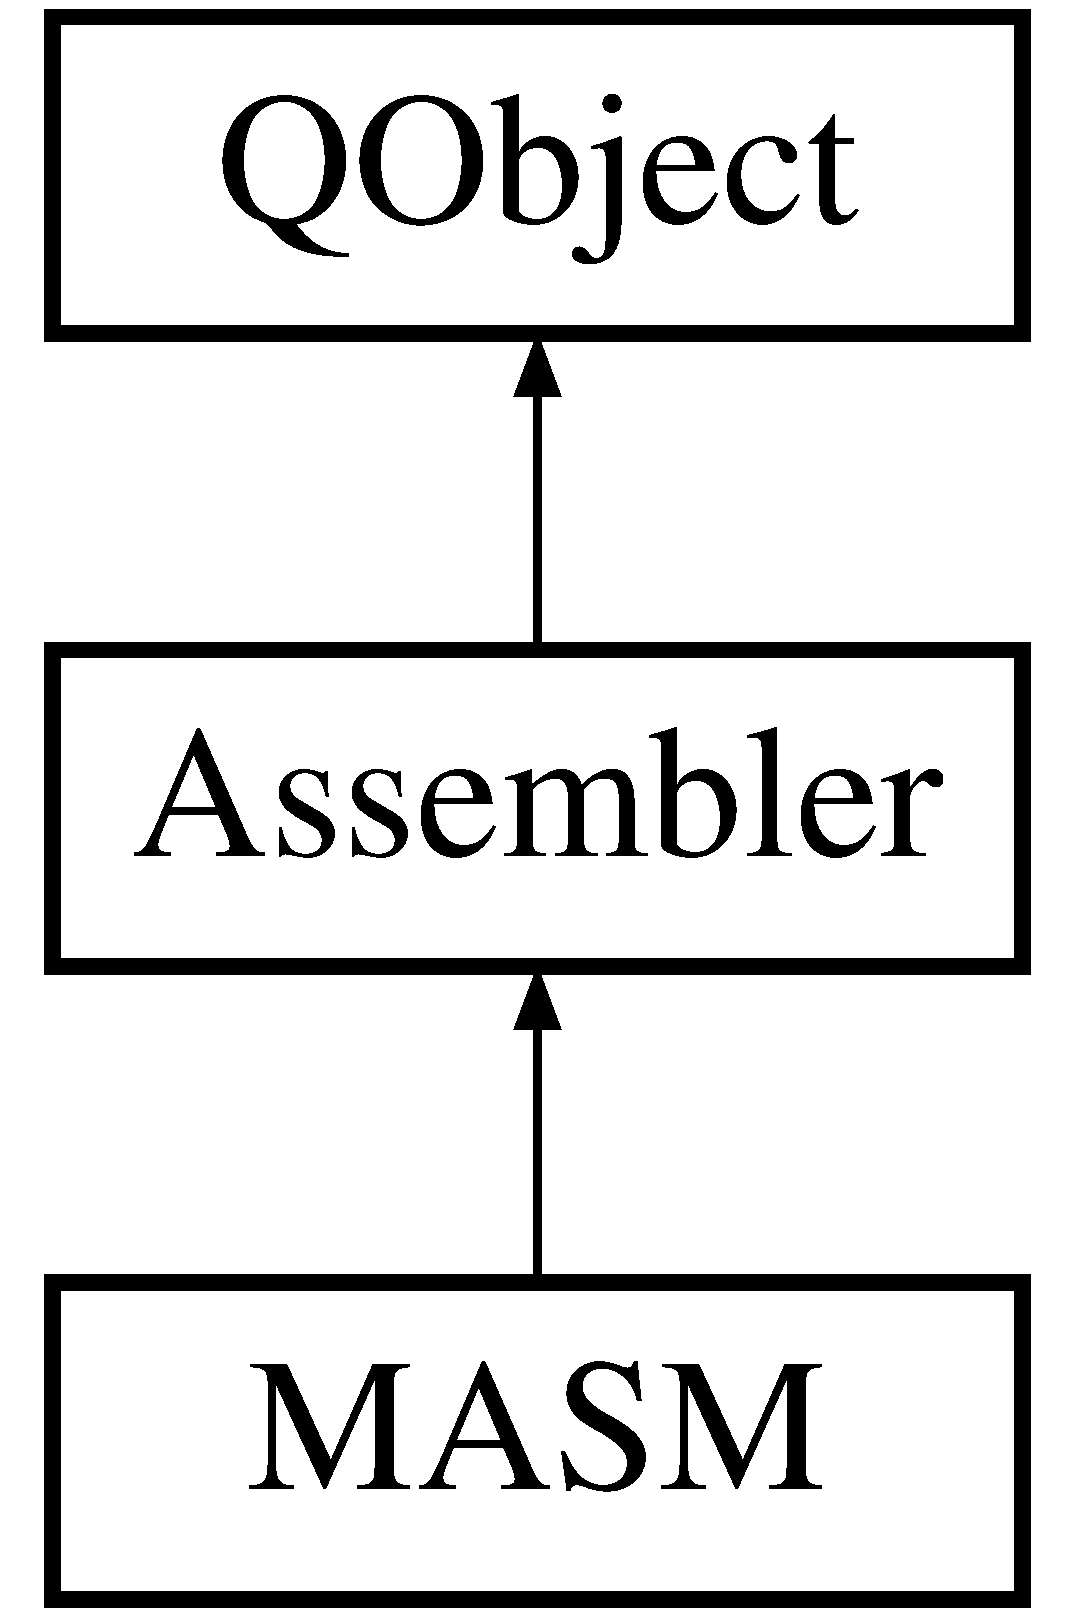
\includegraphics[height=3.000000cm]{class_m_a_s_m}
\end{center}
\end{figure}
\subsection*{Public Member Functions}
\begin{DoxyCompactItemize}
\item 
\hypertarget{class_m_a_s_m_a3dfd4e74baa50b2f7f71c0b1f4f0679f}{}\hyperlink{class_m_a_s_m_a3dfd4e74baa50b2f7f71c0b1f4f0679f}{M\+A\+S\+M} (bool x86, Q\+Object $\ast$parent=0)\label{class_m_a_s_m_a3dfd4e74baa50b2f7f71c0b1f4f0679f}

\begin{DoxyCompactList}\small\item\em Windows only! \end{DoxyCompactList}\item 
\hypertarget{class_m_a_s_m_a22a46b8c03783623be35dc7bb01d3d19}{}Q\+String \hyperlink{class_m_a_s_m_a22a46b8c03783623be35dc7bb01d3d19}{get\+Assembler\+Path} ()\label{class_m_a_s_m_a22a46b8c03783623be35dc7bb01d3d19}

\begin{DoxyCompactList}\small\item\em Return the default path to the assembler. \end{DoxyCompactList}\item 
\hypertarget{class_m_a_s_m_aefccdd4c6d400917163cdd6008e036ff}{}Q\+String \hyperlink{class_m_a_s_m_aefccdd4c6d400917163cdd6008e036ff}{get\+Linker\+Path} ()\label{class_m_a_s_m_aefccdd4c6d400917163cdd6008e036ff}

\begin{DoxyCompactList}\small\item\em Returns the default path to the linker. \end{DoxyCompactList}\item 
quint64 \hyperlink{class_m_a_s_m_aef0f1a5915184bfb9aca890a3493b3ad}{get\+Main\+Offset} (Q\+File \&lst, Q\+String entry\+Label)
\item 
void \hyperlink{class_m_a_s_m_ad52eca298e722cee1e547f62ae24ee11}{parse\+Lst\+File} (Q\+File \&lst, Q\+Vector$<$ \hyperlink{struct_assembler_1_1_line_num}{Assembler\+::\+Line\+Num} $>$ \&lines, quint64 offset)
\item 
void \hyperlink{class_m_a_s_m_a946690c33e0a66a0a91acd857870ffdb}{fill\+Highligher\+Rules} (Q\+Vector$<$ \hyperlink{struct_assembler_1_1_highlighting_rule}{Assembler\+::\+Highlighting\+Rule} $>$ \&highlighting\+Rules, Q\+List$<$ Q\+Text\+Char\+Format $\ast$ $>$ \&formats, bool \&\hyperlink{class_assembler_a8e2ae531c6d59dfea8c7bb90febda262}{multi\+Line\+Comments}, Q\+Reg\+Exp \&comment\+Start\+Expression, Q\+Reg\+Exp \&comment\+End\+Expression)
\item 
\hypertarget{class_m_a_s_m_a9d4eb3151e7082a98db1717203d0835c}{}Q\+String \hyperlink{class_m_a_s_m_a9d4eb3151e7082a98db1717203d0835c}{get\+Start\+Text} ()\label{class_m_a_s_m_a9d4eb3151e7082a98db1717203d0835c}

\begin{DoxyCompactList}\small\item\em Return the default start text (default project code) \end{DoxyCompactList}\item 
\hypertarget{class_m_a_s_m_a915477aac930ce89f5c723557e7edfa4}{}void \hyperlink{class_m_a_s_m_a915477aac930ce89f5c723557e7edfa4}{put\+Debug\+String} (\hyperlink{class_code_editor}{Code\+Editor} $\ast$)\label{class_m_a_s_m_a915477aac930ce89f5c723557e7edfa4}

\begin{DoxyCompactList}\small\item\em Puts the debug string that makes frame (mov ebp, esp) \end{DoxyCompactList}\item 
\hypertarget{class_m_a_s_m_a6b2a173588895bb951992296d80658fc}{}Q\+String \hyperlink{class_m_a_s_m_a6b2a173588895bb951992296d80658fc}{get\+Assembler\+Options} ()\label{class_m_a_s_m_a6b2a173588895bb951992296d80658fc}

\begin{DoxyCompactList}\small\item\em Returns the default assembler options. \end{DoxyCompactList}\item 
\hypertarget{class_m_a_s_m_ae0d538ab3fcaa65e85bab4eb12e6895e}{}Q\+String \hyperlink{class_m_a_s_m_ae0d538ab3fcaa65e85bab4eb12e6895e}{get\+Linker\+Options} ()\label{class_m_a_s_m_ae0d538ab3fcaa65e85bab4eb12e6895e}

\begin{DoxyCompactList}\small\item\em Returns the default linker options. \end{DoxyCompactList}\end{DoxyCompactItemize}
\subsection*{Additional Inherited Members}


\subsection{Detailed Description}
This class defines the behavior for the \hyperlink{class_m_a_s_m}{M\+A\+S\+M} assembler. 



\subsection{Member Function Documentation}
\hypertarget{class_m_a_s_m_a946690c33e0a66a0a91acd857870ffdb}{}\index{M\+A\+S\+M@{M\+A\+S\+M}!fill\+Highligher\+Rules@{fill\+Highligher\+Rules}}
\index{fill\+Highligher\+Rules@{fill\+Highligher\+Rules}!M\+A\+S\+M@{M\+A\+S\+M}}
\subsubsection[{fill\+Highligher\+Rules}]{\setlength{\rightskip}{0pt plus 5cm}void M\+A\+S\+M\+::fill\+Highligher\+Rules (
\begin{DoxyParamCaption}
\item[{Q\+Vector$<$ {\bf Assembler\+::\+Highlighting\+Rule} $>$ \&}]{highlighting\+Rules, }
\item[{Q\+List$<$ Q\+Text\+Char\+Format $\ast$ $>$ \&}]{formats, }
\item[{bool \&}]{multi\+Line\+Comments, }
\item[{Q\+Reg\+Exp \&}]{comment\+Start\+Expression, }
\item[{Q\+Reg\+Exp \&}]{comment\+End\+Expression}
\end{DoxyParamCaption}
)}\label{class_m_a_s_m_a946690c33e0a66a0a91acd857870ffdb}
Setting up regular expressions

Keywords

Memory

Labels

Numbers

Hexadecimal notation

Hexadecimal notation

.labels and numbers with point

System instructions and preprocessor commands \hypertarget{class_m_a_s_m_aef0f1a5915184bfb9aca890a3493b3ad}{}\index{M\+A\+S\+M@{M\+A\+S\+M}!get\+Main\+Offset@{get\+Main\+Offset}}
\index{get\+Main\+Offset@{get\+Main\+Offset}!M\+A\+S\+M@{M\+A\+S\+M}}
\subsubsection[{get\+Main\+Offset}]{\setlength{\rightskip}{0pt plus 5cm}quint64 M\+A\+S\+M\+::get\+Main\+Offset (
\begin{DoxyParamCaption}
\item[{Q\+File \&}]{lst, }
\item[{Q\+String}]{entry\+Label}
\end{DoxyParamCaption}
)\hspace{0.3cm}{\ttfamily [virtual]}}\label{class_m_a_s_m_aef0f1a5915184bfb9aca890a3493b3ad}
get file with listing and name of entry label -\/ main or start. Returns the offset of this label -\/ number of strings and where the label is placed. 

Implements \hyperlink{class_assembler_aa41f46e0cd774718d84bf4e5bd9c65b7}{Assembler}.

\hypertarget{class_m_a_s_m_ad52eca298e722cee1e547f62ae24ee11}{}\index{M\+A\+S\+M@{M\+A\+S\+M}!parse\+Lst\+File@{parse\+Lst\+File}}
\index{parse\+Lst\+File@{parse\+Lst\+File}!M\+A\+S\+M@{M\+A\+S\+M}}
\subsubsection[{parse\+Lst\+File}]{\setlength{\rightskip}{0pt plus 5cm}void M\+A\+S\+M\+::parse\+Lst\+File (
\begin{DoxyParamCaption}
\item[{Q\+File \&}]{lst, }
\item[{Q\+Vector$<$ {\bf Assembler\+::\+Line\+Num} $>$ \&}]{lines, }
\item[{quint64}]{offset}
\end{DoxyParamCaption}
)\hspace{0.3cm}{\ttfamily [virtual]}}\label{class_m_a_s_m_ad52eca298e722cee1e547f62ae24ee11}
Parses the listing file lst and fills Q\+Vector lines with results of parsing. offset -\/ difference between program code in memory and in file. Check if invoke

Check if return

Check if macro

If previous may be macro -\/ switch to finding macro start address mode

If in macro, find its start address

Check if instruction

Offset in instr\+List

Offset in program\+List

If true, skip line in instr\+List and back to first unwatched line in program\+List 

Implements \hyperlink{class_assembler_aa724d277157a407d4d7fd3d0a23e84a7}{Assembler}.



The documentation for this class was generated from the following files\+:\begin{DoxyCompactItemize}
\item 
\hyperlink{masm_8h}{masm.\+h}\item 
\hyperlink{masm_8cpp}{masm.\+cpp}\end{DoxyCompactItemize}

\hypertarget{struct_debugger_1_1memory_info}{}\section{Debugger\+:\+:memory\+Info Struct Reference}
\label{struct_debugger_1_1memory_info}\index{Debugger\+::memory\+Info@{Debugger\+::memory\+Info}}
\subsection*{Public Attributes}
\begin{DoxyCompactItemize}
\item 
\hypertarget{struct_debugger_1_1memory_info_a051ff2fda1d5faa1a188a5e2f3b5b495}{}Q\+String {\bfseries value}\label{struct_debugger_1_1memory_info_a051ff2fda1d5faa1a188a5e2f3b5b495}

\item 
\hypertarget{struct_debugger_1_1memory_info_acf5f4ed0173ad512eece40a70e2095b9}{}bool {\bfseries is\+Valid}\label{struct_debugger_1_1memory_info_acf5f4ed0173ad512eece40a70e2095b9}

\end{DoxyCompactItemize}


The documentation for this struct was generated from the following file\+:\begin{DoxyCompactItemize}
\item 
\hyperlink{debugger_8h}{debugger.\+h}\end{DoxyCompactItemize}

\hypertarget{class_n_a_s_m}{}\section{N\+A\+S\+M Class Reference}
\label{class_n_a_s_m}\index{N\+A\+S\+M@{N\+A\+S\+M}}


This class defines the behavior for the \hyperlink{class_n_a_s_m}{N\+A\+S\+M} assembler.  




{\ttfamily \#include $<$nasm.\+h$>$}

Inheritance diagram for N\+A\+S\+M\+:\begin{figure}[H]
\begin{center}
\leavevmode
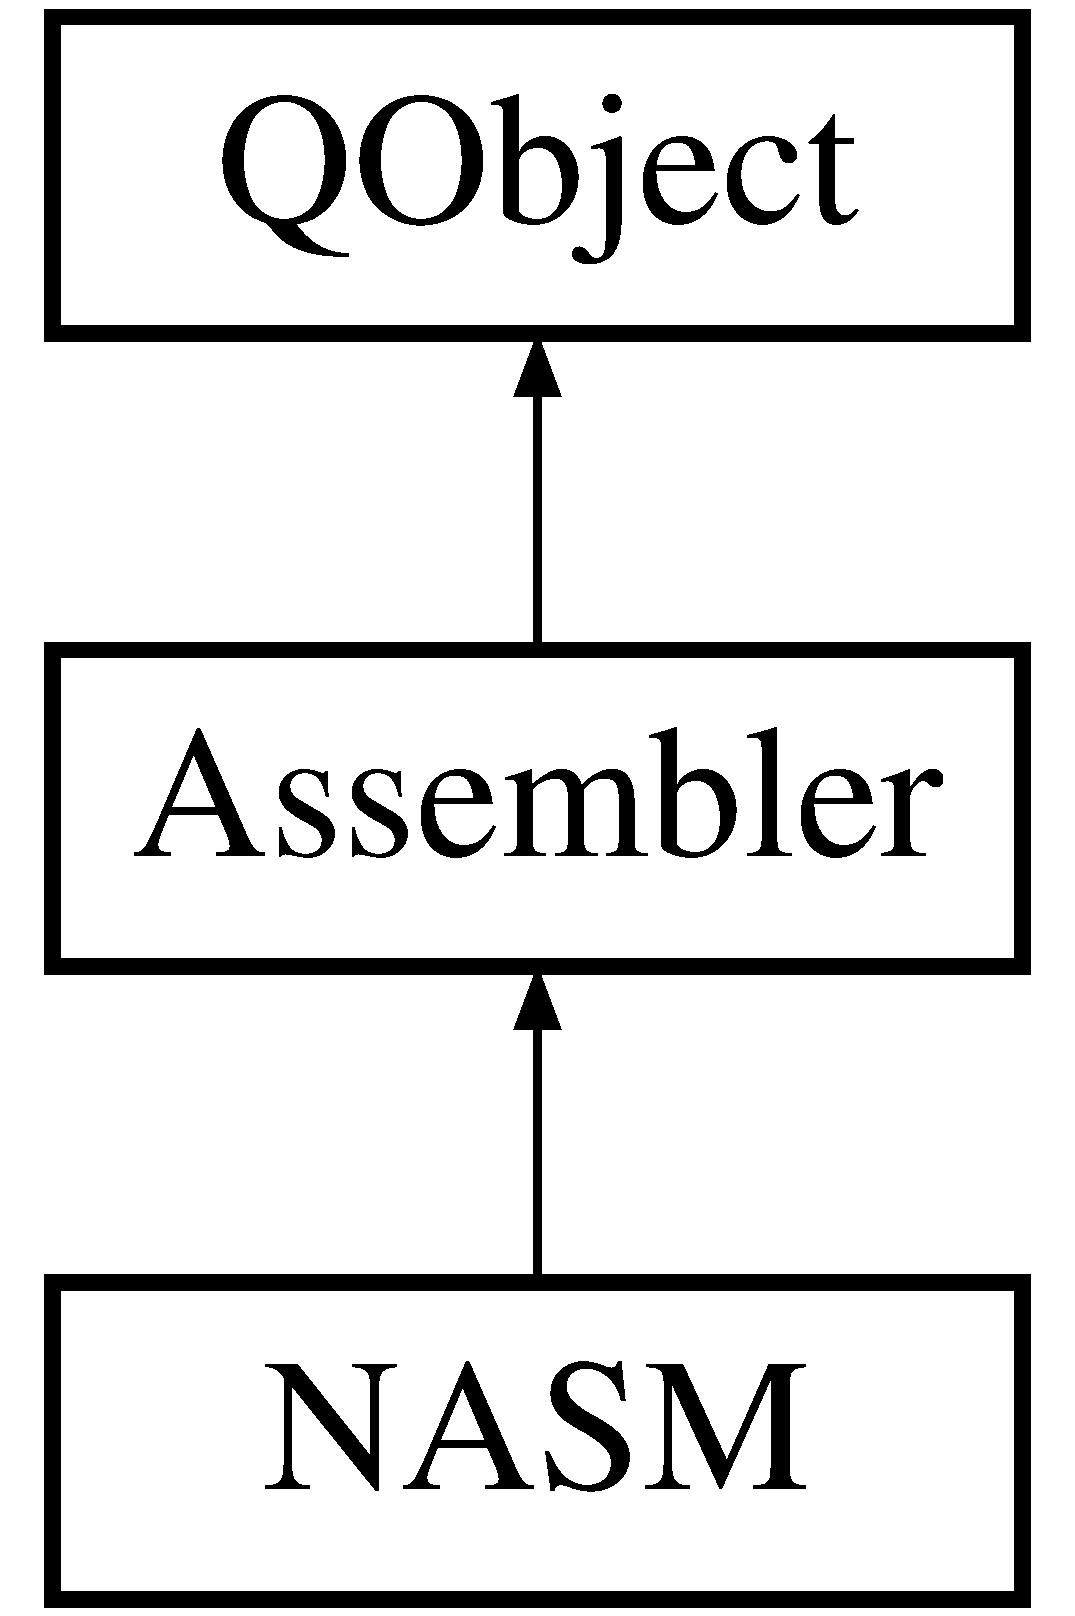
\includegraphics[height=3.000000cm]{class_n_a_s_m}
\end{center}
\end{figure}
\subsection*{Public Member Functions}
\begin{DoxyCompactItemize}
\item 
\hypertarget{class_n_a_s_m_a749bc9c7e08e1a9825c889babced7715}{}{\bfseries N\+A\+S\+M} (bool x86, Q\+Object $\ast$parent=0)\label{class_n_a_s_m_a749bc9c7e08e1a9825c889babced7715}

\item 
\hypertarget{class_n_a_s_m_aaf12100ab23992c4314de00fdb537ab5}{}Q\+String \hyperlink{class_n_a_s_m_aaf12100ab23992c4314de00fdb537ab5}{get\+Assembler\+Path} ()\label{class_n_a_s_m_aaf12100ab23992c4314de00fdb537ab5}

\begin{DoxyCompactList}\small\item\em Return the default path to the assembler. \end{DoxyCompactList}\item 
\hypertarget{class_n_a_s_m_a70cb48d7377086470da91aa2748225c4}{}Q\+String \hyperlink{class_n_a_s_m_a70cb48d7377086470da91aa2748225c4}{get\+Linker\+Path} ()\label{class_n_a_s_m_a70cb48d7377086470da91aa2748225c4}

\begin{DoxyCompactList}\small\item\em Returns the default path to the linker. \end{DoxyCompactList}\item 
quint64 \hyperlink{class_n_a_s_m_a432753e32490e7eaa36d9be41d8f1ed4}{get\+Main\+Offset} (Q\+File \&lst, Q\+String entry\+Label)
\item 
void \hyperlink{class_n_a_s_m_a4de842373fdd8be68c23eb3313ad555e}{parse\+Lst\+File} (Q\+File \&lst, Q\+Vector$<$ \hyperlink{struct_assembler_1_1_line_num}{Assembler\+::\+Line\+Num} $>$ \&lines, quint64 offset)
\item 
void \hyperlink{class_n_a_s_m_abcab860e849ddbfe4ead2baaa09ba592}{fill\+Highligher\+Rules} (Q\+Vector$<$ \hyperlink{struct_assembler_1_1_highlighting_rule}{Assembler\+::\+Highlighting\+Rule} $>$ \&highlighting\+Rules, Q\+List$<$ Q\+Text\+Char\+Format $\ast$ $>$ \&formats, bool \&\hyperlink{class_assembler_a8e2ae531c6d59dfea8c7bb90febda262}{multi\+Line\+Comments}, Q\+Reg\+Exp \&comment\+Start\+Expression, Q\+Reg\+Exp \&comment\+End\+Expression)
\item 
\hypertarget{class_n_a_s_m_ab8b2de6d7f780aeb1962d2fa83e5049f}{}Q\+String \hyperlink{class_n_a_s_m_ab8b2de6d7f780aeb1962d2fa83e5049f}{get\+Start\+Text} ()\label{class_n_a_s_m_ab8b2de6d7f780aeb1962d2fa83e5049f}

\begin{DoxyCompactList}\small\item\em Return the default start text (default project code) \end{DoxyCompactList}\item 
void \hyperlink{class_n_a_s_m_ac4d6d818bc36b8057e21b145480af894}{put\+Debug\+String} (\hyperlink{class_code_editor}{Code\+Editor} $\ast$code)
\begin{DoxyCompactList}\small\item\em Puts the debug string that makes frame (mov ebp, esp) \end{DoxyCompactList}\item 
\hypertarget{class_n_a_s_m_a695bf581a61d6a83235a73c741650ff7}{}Q\+String \hyperlink{class_n_a_s_m_a695bf581a61d6a83235a73c741650ff7}{get\+Assembler\+Options} ()\label{class_n_a_s_m_a695bf581a61d6a83235a73c741650ff7}

\begin{DoxyCompactList}\small\item\em Returns the default assembler options. \end{DoxyCompactList}\item 
\hypertarget{class_n_a_s_m_a6aac9e3f8fa1f9243d4f4fe44f82ffb4}{}Q\+String \hyperlink{class_n_a_s_m_a6aac9e3f8fa1f9243d4f4fe44f82ffb4}{get\+Linker\+Options} ()\label{class_n_a_s_m_a6aac9e3f8fa1f9243d4f4fe44f82ffb4}

\begin{DoxyCompactList}\small\item\em Returns the default linker options. \end{DoxyCompactList}\end{DoxyCompactItemize}
\subsection*{Additional Inherited Members}


\subsection{Detailed Description}
This class defines the behavior for the \hyperlink{class_n_a_s_m}{N\+A\+S\+M} assembler. 



\subsection{Member Function Documentation}
\hypertarget{class_n_a_s_m_abcab860e849ddbfe4ead2baaa09ba592}{}\index{N\+A\+S\+M@{N\+A\+S\+M}!fill\+Highligher\+Rules@{fill\+Highligher\+Rules}}
\index{fill\+Highligher\+Rules@{fill\+Highligher\+Rules}!N\+A\+S\+M@{N\+A\+S\+M}}
\subsubsection[{fill\+Highligher\+Rules}]{\setlength{\rightskip}{0pt plus 5cm}void N\+A\+S\+M\+::fill\+Highligher\+Rules (
\begin{DoxyParamCaption}
\item[{Q\+Vector$<$ {\bf Assembler\+::\+Highlighting\+Rule} $>$ \&}]{highlighting\+Rules, }
\item[{Q\+List$<$ Q\+Text\+Char\+Format $\ast$ $>$ \&}]{formats, }
\item[{bool \&}]{multi\+Line\+Comments, }
\item[{Q\+Reg\+Exp \&}]{comment\+Start\+Expression, }
\item[{Q\+Reg\+Exp \&}]{comment\+End\+Expression}
\end{DoxyParamCaption}
)}\label{class_n_a_s_m_abcab860e849ddbfe4ead2baaa09ba592}
Setting up regular expressions

Keywords

I\+O macros

Memory

Labels

Numbers

Registers

Labels and numbers with point

System instructions and preprocessor commands

Quotations

Comments \hypertarget{class_n_a_s_m_a432753e32490e7eaa36d9be41d8f1ed4}{}\index{N\+A\+S\+M@{N\+A\+S\+M}!get\+Main\+Offset@{get\+Main\+Offset}}
\index{get\+Main\+Offset@{get\+Main\+Offset}!N\+A\+S\+M@{N\+A\+S\+M}}
\subsubsection[{get\+Main\+Offset}]{\setlength{\rightskip}{0pt plus 5cm}quint64 N\+A\+S\+M\+::get\+Main\+Offset (
\begin{DoxyParamCaption}
\item[{Q\+File \&}]{lst, }
\item[{Q\+String}]{entry\+Label}
\end{DoxyParamCaption}
)\hspace{0.3cm}{\ttfamily [virtual]}}\label{class_n_a_s_m_a432753e32490e7eaa36d9be41d8f1ed4}
get file with listing and name of entry label -\/ main or start. Returns the offset of this label -\/ number of strings and where the label is placed. Omit strings with data only if in list \+: line number, address, data and it is all (without instruction) -\/ omit this string

Exclude 0 0 

Implements \hyperlink{class_assembler_aa41f46e0cd774718d84bf4e5bd9c65b7}{Assembler}.

\hypertarget{class_n_a_s_m_a4de842373fdd8be68c23eb3313ad555e}{}\index{N\+A\+S\+M@{N\+A\+S\+M}!parse\+Lst\+File@{parse\+Lst\+File}}
\index{parse\+Lst\+File@{parse\+Lst\+File}!N\+A\+S\+M@{N\+A\+S\+M}}
\subsubsection[{parse\+Lst\+File}]{\setlength{\rightskip}{0pt plus 5cm}void N\+A\+S\+M\+::parse\+Lst\+File (
\begin{DoxyParamCaption}
\item[{Q\+File \&}]{lst, }
\item[{Q\+Vector$<$ {\bf Assembler\+::\+Line\+Num} $>$ \&}]{lines, }
\item[{quint64}]{offset}
\end{DoxyParamCaption}
)\hspace{0.3cm}{\ttfamily [virtual]}}\label{class_n_a_s_m_a4de842373fdd8be68c23eb3313ad555e}
Parses the listing file lst and fills Q\+Vector lines with results of parsing. offset -\/ difference between program code in memory and in file. omit strings with data only if in list \+: line number, address, data and it is all (without instruction) -\/ omit this string and subtract 1 from offset

Offset in list 

Implements \hyperlink{class_assembler_aa724d277157a407d4d7fd3d0a23e84a7}{Assembler}.

\hypertarget{class_n_a_s_m_ac4d6d818bc36b8057e21b145480af894}{}\index{N\+A\+S\+M@{N\+A\+S\+M}!put\+Debug\+String@{put\+Debug\+String}}
\index{put\+Debug\+String@{put\+Debug\+String}!N\+A\+S\+M@{N\+A\+S\+M}}
\subsubsection[{put\+Debug\+String}]{\setlength{\rightskip}{0pt plus 5cm}void N\+A\+S\+M\+::put\+Debug\+String (
\begin{DoxyParamCaption}
\item[{{\bf Code\+Editor} $\ast$}]{code}
\end{DoxyParamCaption}
)\hspace{0.3cm}{\ttfamily [virtual]}}\label{class_n_a_s_m_ac4d6d818bc36b8057e21b145480af894}


Puts the debug string that makes frame (mov ebp, esp) 

add \+: mov ebp, esp for making frame for correct debugging if this code has not been added yet 

Implements \hyperlink{class_assembler_a3d699b729df36103f37a8ac45d54a0a6}{Assembler}.



The documentation for this class was generated from the following files\+:\begin{DoxyCompactItemize}
\item 
\hyperlink{nasm_8h}{nasm.\+h}\item 
\hyperlink{nasm_8cpp}{nasm.\+cpp}\end{DoxyCompactItemize}

\hypertarget{struct_debugger_1_1registers_info}{}\section{Debugger\+:\+:registers\+Info Struct Reference}
\label{struct_debugger_1_1registers_info}\index{Debugger\+::registers\+Info@{Debugger\+::registers\+Info}}
\subsection*{Public Attributes}
\begin{DoxyCompactItemize}
\item 
\hypertarget{struct_debugger_1_1registers_info_ae3b2f5a8a3067a3c918b49bf1199cd3d}{}Q\+String {\bfseries name}\label{struct_debugger_1_1registers_info_ae3b2f5a8a3067a3c918b49bf1199cd3d}

\item 
\hypertarget{struct_debugger_1_1registers_info_a339a32649de1b03fcde0a970c44f8d58}{}Q\+String {\bfseries hex\+Value}\label{struct_debugger_1_1registers_info_a339a32649de1b03fcde0a970c44f8d58}

\item 
\hypertarget{struct_debugger_1_1registers_info_a9d6dbc77e7e94f55dc89c72798f70d2f}{}Q\+String {\bfseries dec\+Value}\label{struct_debugger_1_1registers_info_a9d6dbc77e7e94f55dc89c72798f70d2f}

\end{DoxyCompactItemize}


The documentation for this struct was generated from the following file\+:\begin{DoxyCompactItemize}
\item 
\hyperlink{debugger_8h}{debugger.\+h}\end{DoxyCompactItemize}

\hypertarget{class_ru_q_plain_text_edit}{}\section{Ru\+Q\+Plain\+Text\+Edit Class Reference}
\label{class_ru_q_plain_text_edit}\index{Ru\+Q\+Plain\+Text\+Edit@{Ru\+Q\+Plain\+Text\+Edit}}


This defines the base class which the text editor is derived from.  




{\ttfamily \#include $<$ruqplaintextedit.\+h$>$}

Inheritance diagram for Ru\+Q\+Plain\+Text\+Edit\+:\begin{figure}[H]
\begin{center}
\leavevmode
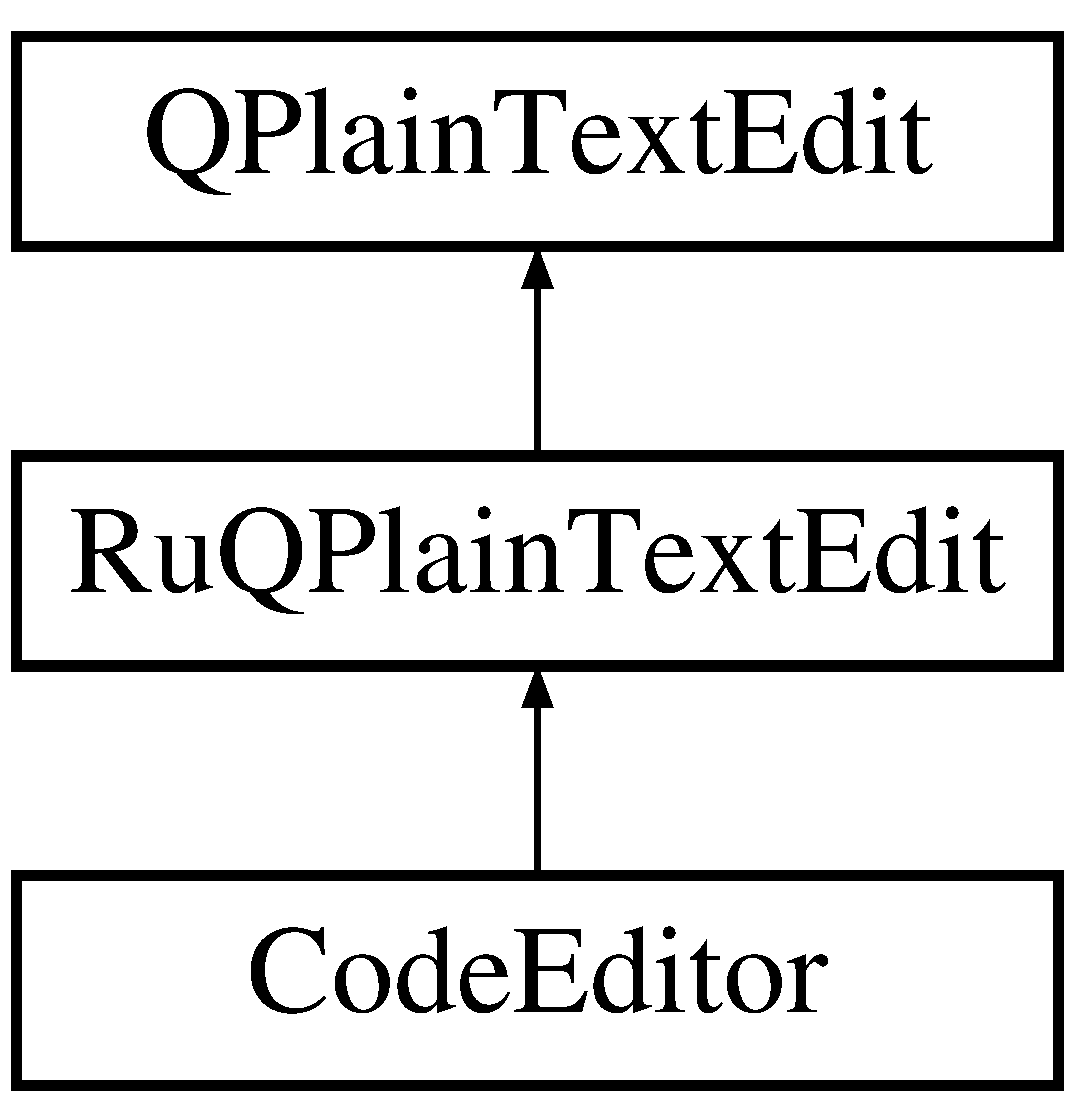
\includegraphics[height=3.000000cm]{class_ru_q_plain_text_edit}
\end{center}
\end{figure}
\subsection*{Classes}
\begin{DoxyCompactItemize}
\item 
struct \hyperlink{struct_ru_q_plain_text_edit_1_1_watch}{Watch}
\begin{DoxyCompactList}\small\item\em Defines a structure to keep track of a watched variable. \end{DoxyCompactList}\end{DoxyCompactItemize}
\subsection*{Public Slots}
\begin{DoxyCompactItemize}
\item 
\hypertarget{class_ru_q_plain_text_edit_aa4304c1935d62a21ca47caefcb4fe73a}{}void \hyperlink{class_ru_q_plain_text_edit_aa4304c1935d62a21ca47caefcb4fe73a}{comment\+Selected\+Code} ()\label{class_ru_q_plain_text_edit_aa4304c1935d62a21ca47caefcb4fe73a}

\begin{DoxyCompactList}\small\item\em Method that comments the user selected code. \end{DoxyCompactList}\item 
\hypertarget{class_ru_q_plain_text_edit_ae4261c2f4317d73e210fb4307291c336}{}void \hyperlink{class_ru_q_plain_text_edit_ae4261c2f4317d73e210fb4307291c336}{uncomment\+Selected\+Code} ()\label{class_ru_q_plain_text_edit_ae4261c2f4317d73e210fb4307291c336}

\begin{DoxyCompactList}\small\item\em Method for uncommenting a previously commented code block. \end{DoxyCompactList}\item 
\hypertarget{class_ru_q_plain_text_edit_a2b37f59c4986e846036b5626fc635e84}{}void {\bfseries delete\+Selected} ()\label{class_ru_q_plain_text_edit_a2b37f59c4986e846036b5626fc635e84}

\item 
\hypertarget{class_ru_q_plain_text_edit_abe44143e74b70e76b7c098378cdce21f}{}void \hyperlink{class_ru_q_plain_text_edit_abe44143e74b70e76b7c098378cdce21f}{add\+Watch} ()\label{class_ru_q_plain_text_edit_abe44143e74b70e76b7c098378cdce21f}

\begin{DoxyCompactList}\small\item\em Method for adding a variable watch. \end{DoxyCompactList}\item 
\hypertarget{class_ru_q_plain_text_edit_a4c8f22184407d5d9cd402e9e19a77dfa}{}void \hyperlink{class_ru_q_plain_text_edit_a4c8f22184407d5d9cd402e9e19a77dfa}{set\+Debug\+Enabled} ()\label{class_ru_q_plain_text_edit_a4c8f22184407d5d9cd402e9e19a77dfa}

\begin{DoxyCompactList}\small\item\em Used to enable the debugger. \end{DoxyCompactList}\item 
\hypertarget{class_ru_q_plain_text_edit_a941b8becef86d6c5a9378843d084e67a}{}void \hyperlink{class_ru_q_plain_text_edit_a941b8becef86d6c5a9378843d084e67a}{set\+Debug\+Disabled} ()\label{class_ru_q_plain_text_edit_a941b8becef86d6c5a9378843d084e67a}

\begin{DoxyCompactList}\small\item\em Used to disable the debugger. \end{DoxyCompactList}\end{DoxyCompactItemize}
\subsection*{Signals}
\begin{DoxyCompactItemize}
\item 
\hypertarget{class_ru_q_plain_text_edit_a91e38e4be24851ce670ecf4d22965f1b}{}void \hyperlink{class_ru_q_plain_text_edit_a91e38e4be24851ce670ecf4d22965f1b}{add\+Watch\+Signal} (\hyperlink{struct_ru_q_plain_text_edit_1_1_watch}{Ru\+Q\+Plain\+Text\+Edit\+::\+Watch} variable)\label{class_ru_q_plain_text_edit_a91e38e4be24851ce670ecf4d22965f1b}

\begin{DoxyCompactList}\small\item\em U\+N\+K\+N\+O\+W\+N. \end{DoxyCompactList}\end{DoxyCompactItemize}
\subsection*{Public Member Functions}
\begin{DoxyCompactItemize}
\item 
\hypertarget{class_ru_q_plain_text_edit_a793cf95c0462ad8ae738c975d5f548ef}{}\hyperlink{class_ru_q_plain_text_edit_a793cf95c0462ad8ae738c975d5f548ef}{Ru\+Q\+Plain\+Text\+Edit} (Q\+Widget $\ast$parent=0)\label{class_ru_q_plain_text_edit_a793cf95c0462ad8ae738c975d5f548ef}

\begin{DoxyCompactList}\small\item\em The class constructor creates the editor, given a specified parent Q\+Widget object. \end{DoxyCompactList}\item 
Q\+Menu $\ast$ \hyperlink{class_ru_q_plain_text_edit_aad91c0ff3e7c3dede14ee0f6eb05afee}{create\+Menu} ()
\begin{DoxyCompactList}\small\item\em Creates a menu. \end{DoxyCompactList}\end{DoxyCompactItemize}
\subsection*{Protected Member Functions}
\begin{DoxyCompactItemize}
\item 
\hypertarget{class_ru_q_plain_text_edit_a3ebf1e882b641ceebd106c7fa44d0a2f}{}void {\bfseries context\+Menu\+Event} (Q\+Context\+Menu\+Event $\ast$e)\label{class_ru_q_plain_text_edit_a3ebf1e882b641ceebd106c7fa44d0a2f}

\end{DoxyCompactItemize}
\subsection*{Private Member Functions}
\begin{DoxyCompactItemize}
\item 
\hypertarget{class_ru_q_plain_text_edit_abbbaf9221ce9a2da5dc0465099080f01}{}\hyperlink{struct_ru_q_plain_text_edit_1_1_watch}{Ru\+Q\+Plain\+Text\+Edit\+::\+Watch} {\bfseries variable\+On\+Current\+Line} ()\label{class_ru_q_plain_text_edit_abbbaf9221ce9a2da5dc0465099080f01}

\end{DoxyCompactItemize}
\subsection*{Private Attributes}
\begin{DoxyCompactItemize}
\item 
\hypertarget{class_ru_q_plain_text_edit_aa8b913265b0dc3aa6da202073896ab14}{}Q\+Pointer$<$ Q\+Menu $>$ {\bfseries context\+Menu}\label{class_ru_q_plain_text_edit_aa8b913265b0dc3aa6da202073896ab14}

\item 
\hypertarget{class_ru_q_plain_text_edit_a2b8d4092c92e175127d1352da14a3f78}{}Q\+Action $\ast$ \hyperlink{class_ru_q_plain_text_edit_a2b8d4092c92e175127d1352da14a3f78}{comment\+Action}\label{class_ru_q_plain_text_edit_a2b8d4092c92e175127d1352da14a3f78}

\begin{DoxyCompactList}\small\item\em Creates a comment. \end{DoxyCompactList}\item 
\hypertarget{class_ru_q_plain_text_edit_a38538d75910f8e62955cba9bafbc6862}{}Q\+Action $\ast$ \hyperlink{class_ru_q_plain_text_edit_a38538d75910f8e62955cba9bafbc6862}{uncomment\+Action}\label{class_ru_q_plain_text_edit_a38538d75910f8e62955cba9bafbc6862}

\begin{DoxyCompactList}\small\item\em Removes a comment. \end{DoxyCompactList}\item 
\hypertarget{class_ru_q_plain_text_edit_a05683430c4f10aae97088275bab17b87}{}Q\+Action $\ast$ \hyperlink{class_ru_q_plain_text_edit_a05683430c4f10aae97088275bab17b87}{undo\+Action}\label{class_ru_q_plain_text_edit_a05683430c4f10aae97088275bab17b87}

\begin{DoxyCompactList}\small\item\em Undo the last action. \end{DoxyCompactList}\item 
\hypertarget{class_ru_q_plain_text_edit_af29953e5a06920e1ba6eb1da9be7ca1e}{}Q\+Action $\ast$ \hyperlink{class_ru_q_plain_text_edit_af29953e5a06920e1ba6eb1da9be7ca1e}{redo\+Action}\label{class_ru_q_plain_text_edit_af29953e5a06920e1ba6eb1da9be7ca1e}

\begin{DoxyCompactList}\small\item\em Do the previous action again. \end{DoxyCompactList}\item 
\hypertarget{class_ru_q_plain_text_edit_a3c6a96c2287b9a2b58b739468c40d367}{}Q\+Action $\ast$ \hyperlink{class_ru_q_plain_text_edit_a3c6a96c2287b9a2b58b739468c40d367}{cut\+Action}\label{class_ru_q_plain_text_edit_a3c6a96c2287b9a2b58b739468c40d367}

\begin{DoxyCompactList}\small\item\em Cut a selected text string. \end{DoxyCompactList}\item 
\hypertarget{class_ru_q_plain_text_edit_a19d8b06c4d6b3a2fe7f5b3a675403d03}{}Q\+Action $\ast$ \hyperlink{class_ru_q_plain_text_edit_a19d8b06c4d6b3a2fe7f5b3a675403d03}{copy\+Action}\label{class_ru_q_plain_text_edit_a19d8b06c4d6b3a2fe7f5b3a675403d03}

\begin{DoxyCompactList}\small\item\em Copy a selected text string. \end{DoxyCompactList}\item 
\hypertarget{class_ru_q_plain_text_edit_ab5ab9d30f4a05b5371444ab7fde9927b}{}Q\+Action $\ast$ \hyperlink{class_ru_q_plain_text_edit_ab5ab9d30f4a05b5371444ab7fde9927b}{paste\+Action}\label{class_ru_q_plain_text_edit_ab5ab9d30f4a05b5371444ab7fde9927b}

\begin{DoxyCompactList}\small\item\em Pase the clipboard contents. \end{DoxyCompactList}\item 
\hypertarget{class_ru_q_plain_text_edit_ad040e7e27a980e1bb67505fc3dbe9f8a}{}Q\+Action $\ast$ \hyperlink{class_ru_q_plain_text_edit_ad040e7e27a980e1bb67505fc3dbe9f8a}{delete\+Action}\label{class_ru_q_plain_text_edit_ad040e7e27a980e1bb67505fc3dbe9f8a}

\begin{DoxyCompactList}\small\item\em U\+N\+K\+N\+O\+W\+N. \end{DoxyCompactList}\item 
\hypertarget{class_ru_q_plain_text_edit_ae0aadce86a565814f15660816d7eaced}{}Q\+Action $\ast$ \hyperlink{class_ru_q_plain_text_edit_ae0aadce86a565814f15660816d7eaced}{select\+All\+Action}\label{class_ru_q_plain_text_edit_ae0aadce86a565814f15660816d7eaced}

\begin{DoxyCompactList}\small\item\em Select all of the text. \end{DoxyCompactList}\item 
\hypertarget{class_ru_q_plain_text_edit_a58f97203281130df24c917791730bbaa}{}Q\+Action $\ast$ \hyperlink{class_ru_q_plain_text_edit_a58f97203281130df24c917791730bbaa}{add\+Watch\+Action}\label{class_ru_q_plain_text_edit_a58f97203281130df24c917791730bbaa}

\begin{DoxyCompactList}\small\item\em Add a watch on a variable. \end{DoxyCompactList}\item 
\hypertarget{class_ru_q_plain_text_edit_a741b5b182b316358df02611a21933ec1}{}bool \hyperlink{class_ru_q_plain_text_edit_a741b5b182b316358df02611a21933ec1}{debug\+Enabled}\label{class_ru_q_plain_text_edit_a741b5b182b316358df02611a21933ec1}

\begin{DoxyCompactList}\small\item\em Used to keep track if the debugger is enabled. \end{DoxyCompactList}\end{DoxyCompactItemize}


\subsection{Detailed Description}
This defines the base class which the text editor is derived from. 

The class contains methods that are used in the editor. These range from simple copying and pasting to enabling/disabling the debugger. 

\subsection{Member Function Documentation}
\hypertarget{class_ru_q_plain_text_edit_aad91c0ff3e7c3dede14ee0f6eb05afee}{}\index{Ru\+Q\+Plain\+Text\+Edit@{Ru\+Q\+Plain\+Text\+Edit}!create\+Menu@{create\+Menu}}
\index{create\+Menu@{create\+Menu}!Ru\+Q\+Plain\+Text\+Edit@{Ru\+Q\+Plain\+Text\+Edit}}
\subsubsection[{create\+Menu}]{\setlength{\rightskip}{0pt plus 5cm}Q\+Menu $\ast$ Ru\+Q\+Plain\+Text\+Edit\+::create\+Menu (
\begin{DoxyParamCaption}
{}
\end{DoxyParamCaption}
)}\label{class_ru_q_plain_text_edit_aad91c0ff3e7c3dede14ee0f6eb05afee}


Creates a menu. 

if nothing selected 

The documentation for this class was generated from the following files\+:\begin{DoxyCompactItemize}
\item 
\hyperlink{ruqplaintextedit_8h}{ruqplaintextedit.\+h}\item 
ruqplaintextedit.\+cpp\end{DoxyCompactItemize}

\hypertarget{class_ru_q_text_edit}{}\section{Ru\+Q\+Text\+Edit Class Reference}
\label{class_ru_q_text_edit}\index{Ru\+Q\+Text\+Edit@{Ru\+Q\+Text\+Edit}}


The \hyperlink{class_ru_q_text_edit}{Ru\+Q\+Text\+Edit} defines the methods specified by Q\+T's Q\+Text\+Edit class. These are things like copying/pasting, edit, undo, etc...  




{\ttfamily \#include $<$ruqtextedit.\+h$>$}

Inheritance diagram for Ru\+Q\+Text\+Edit\+:\begin{figure}[H]
\begin{center}
\leavevmode
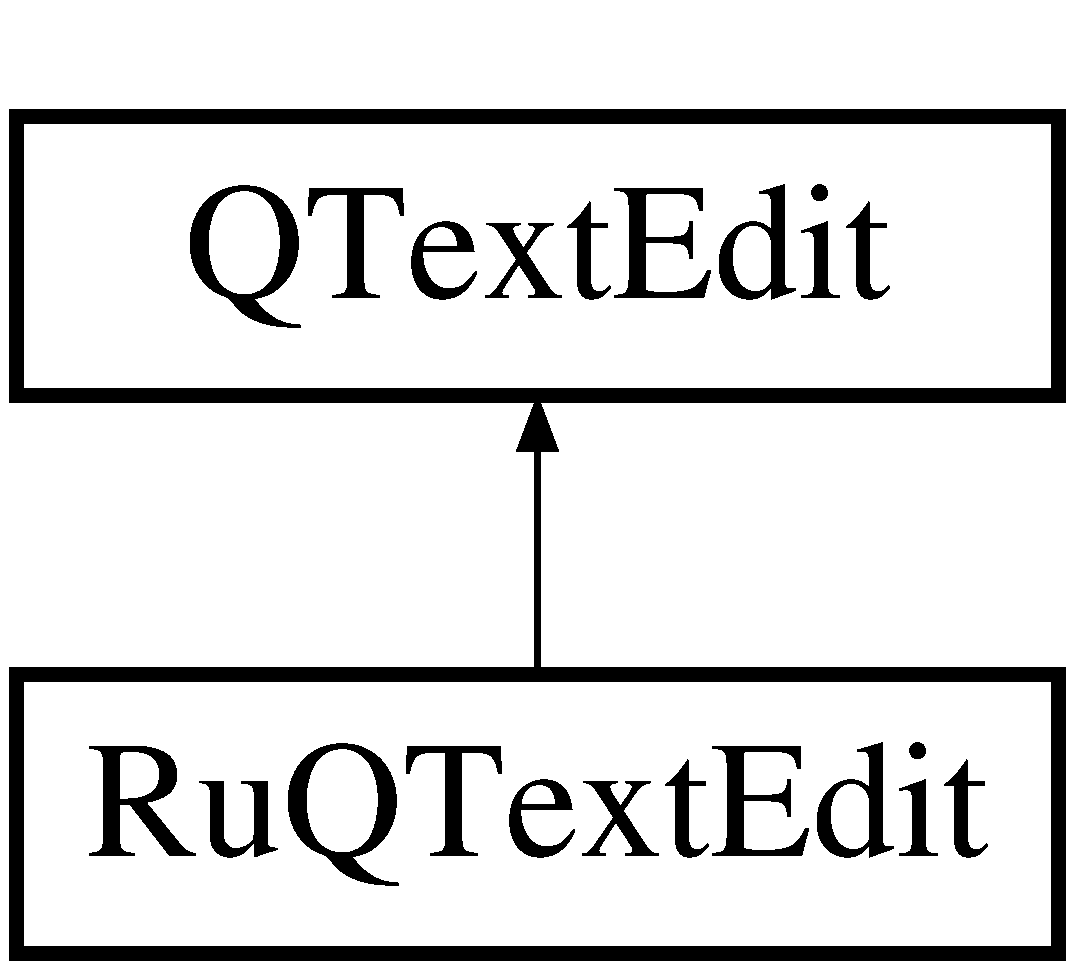
\includegraphics[height=2.000000cm]{class_ru_q_text_edit}
\end{center}
\end{figure}
\subsection*{Public Slots}
\begin{DoxyCompactItemize}
\item 
\hypertarget{class_ru_q_text_edit_a77cd67f6d9eebf4054c96d213872f97f}{}void {\bfseries delete\+Selected} ()\label{class_ru_q_text_edit_a77cd67f6d9eebf4054c96d213872f97f}

\end{DoxyCompactItemize}
\subsection*{Public Member Functions}
\begin{DoxyCompactItemize}
\item 
\hypertarget{class_ru_q_text_edit_a856a9951b1d7b989c5150f9dc2a387d3}{}{\bfseries Ru\+Q\+Text\+Edit} (Q\+Widget $\ast$parent=0)\label{class_ru_q_text_edit_a856a9951b1d7b989c5150f9dc2a387d3}

\end{DoxyCompactItemize}
\subsection*{Protected Member Functions}
\begin{DoxyCompactItemize}
\item 
void \hyperlink{class_ru_q_text_edit_a8fc9c19a6eed33f89d0d62d23ec57ca9}{context\+Menu\+Event} (Q\+Context\+Menu\+Event $\ast$e)
\end{DoxyCompactItemize}
\subsection*{Private Attributes}
\begin{DoxyCompactItemize}
\item 
\hypertarget{class_ru_q_text_edit_aae1b11fbabd5cc5a6d83f0e8b0013965}{}Q\+Pointer$<$ Q\+Menu $>$ {\bfseries context\+Menu}\label{class_ru_q_text_edit_aae1b11fbabd5cc5a6d83f0e8b0013965}

\item 
\hypertarget{class_ru_q_text_edit_a72a48f39790a5f7b559c501c0caa153d}{}Q\+Action $\ast$ {\bfseries undo\+Action}\label{class_ru_q_text_edit_a72a48f39790a5f7b559c501c0caa153d}

\item 
\hypertarget{class_ru_q_text_edit_a7b2b190d834ac530192f58b09ddd5c21}{}Q\+Action $\ast$ {\bfseries redo\+Action}\label{class_ru_q_text_edit_a7b2b190d834ac530192f58b09ddd5c21}

\item 
\hypertarget{class_ru_q_text_edit_ac1b1b077f5d46920f273403768b9893b}{}Q\+Action $\ast$ {\bfseries cut\+Action}\label{class_ru_q_text_edit_ac1b1b077f5d46920f273403768b9893b}

\item 
\hypertarget{class_ru_q_text_edit_ab267bc74de48b1f546917739084d28a4}{}Q\+Action $\ast$ {\bfseries copy\+Action}\label{class_ru_q_text_edit_ab267bc74de48b1f546917739084d28a4}

\item 
\hypertarget{class_ru_q_text_edit_aa978383f49eabf0ac51066c321c21248}{}Q\+Action $\ast$ {\bfseries paste\+Action}\label{class_ru_q_text_edit_aa978383f49eabf0ac51066c321c21248}

\item 
\hypertarget{class_ru_q_text_edit_ad049ff4284897924607c429e15243cf7}{}Q\+Action $\ast$ {\bfseries delete\+Action}\label{class_ru_q_text_edit_ad049ff4284897924607c429e15243cf7}

\item 
\hypertarget{class_ru_q_text_edit_ae6c0886a95235ca04f7873f73997ecab}{}Q\+Action $\ast$ {\bfseries select\+All\+Action}\label{class_ru_q_text_edit_ae6c0886a95235ca04f7873f73997ecab}

\item 
\hypertarget{class_ru_q_text_edit_a873f730061faeca79d8fadd6f5f18556}{}Q\+Action $\ast$ {\bfseries clear\+Action}\label{class_ru_q_text_edit_a873f730061faeca79d8fadd6f5f18556}

\end{DoxyCompactItemize}


\subsection{Detailed Description}
The \hyperlink{class_ru_q_text_edit}{Ru\+Q\+Text\+Edit} defines the methods specified by Q\+T's Q\+Text\+Edit class. These are things like copying/pasting, edit, undo, etc... 



\subsection{Member Function Documentation}
\hypertarget{class_ru_q_text_edit_a8fc9c19a6eed33f89d0d62d23ec57ca9}{}\index{Ru\+Q\+Text\+Edit@{Ru\+Q\+Text\+Edit}!context\+Menu\+Event@{context\+Menu\+Event}}
\index{context\+Menu\+Event@{context\+Menu\+Event}!Ru\+Q\+Text\+Edit@{Ru\+Q\+Text\+Edit}}
\subsubsection[{context\+Menu\+Event}]{\setlength{\rightskip}{0pt plus 5cm}void Ru\+Q\+Text\+Edit\+::context\+Menu\+Event (
\begin{DoxyParamCaption}
\item[{Q\+Context\+Menu\+Event $\ast$}]{e}
\end{DoxyParamCaption}
)\hspace{0.3cm}{\ttfamily [protected]}}\label{class_ru_q_text_edit_a8fc9c19a6eed33f89d0d62d23ec57ca9}
if nothing selected 

The documentation for this class was generated from the following files\+:\begin{DoxyCompactItemize}
\item 
\hyperlink{ruqtextedit_8h}{ruqtextedit.\+h}\item 
\hyperlink{ruqtextedit_8cpp}{ruqtextedit.\+cpp}\end{DoxyCompactItemize}

\hypertarget{class_signal_locker}{}\section{Signal\+Locker Class Reference}
\label{class_signal_locker}\index{Signal\+Locker@{Signal\+Locker}}


U\+N\+K\+N\+O\+W\+N.  




{\ttfamily \#include $<$signallocker.\+h$>$}

Inheritance diagram for Signal\+Locker\+:\begin{figure}[H]
\begin{center}
\leavevmode
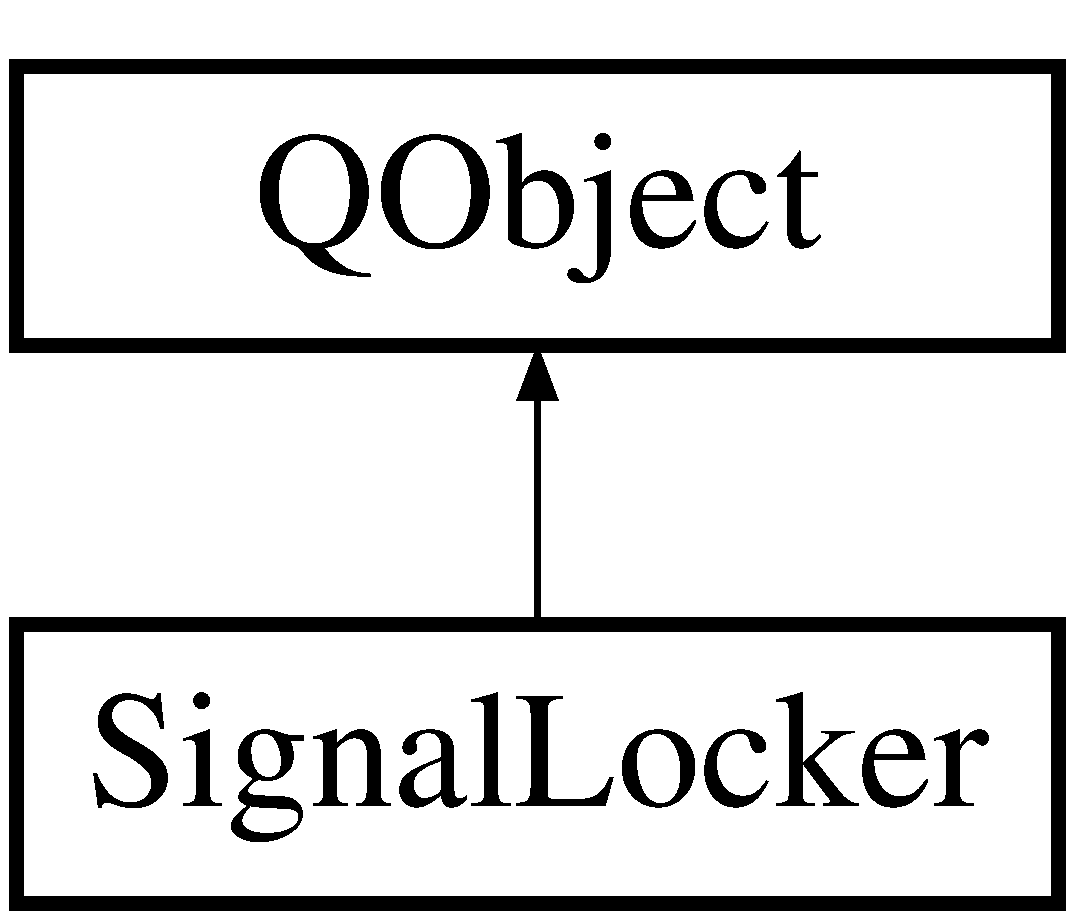
\includegraphics[height=2.000000cm]{class_signal_locker}
\end{center}
\end{figure}
\subsection*{Public Slots}
\begin{DoxyCompactItemize}
\item 
\hypertarget{class_signal_locker_a9cc13c97b47bc5329eb87fbeb39c8c21}{}void {\bfseries unlock} ()\label{class_signal_locker_a9cc13c97b47bc5329eb87fbeb39c8c21}

\item 
\hypertarget{class_signal_locker_a4580211e877dc365f58523a887903f54}{}bool {\bfseries try\+Lock} ()\label{class_signal_locker_a4580211e877dc365f58523a887903f54}

\item 
\hypertarget{class_signal_locker_a0e083bc4b1d1a0eb2561c898357d79f5}{}void {\bfseries lock} ()\label{class_signal_locker_a0e083bc4b1d1a0eb2561c898357d79f5}

\end{DoxyCompactItemize}
\subsection*{Public Member Functions}
\begin{DoxyCompactItemize}
\item 
\hypertarget{class_signal_locker_a2fa8c9dc5a14f60e7c3851bca19b1ddc}{}{\bfseries Signal\+Locker} (Q\+Object $\ast$parent=0)\label{class_signal_locker_a2fa8c9dc5a14f60e7c3851bca19b1ddc}

\end{DoxyCompactItemize}
\subsection*{Private Attributes}
\begin{DoxyCompactItemize}
\item 
\hypertarget{class_signal_locker_a0e96113a0a1a6244d75ec4445096b0ab}{}bool {\bfseries locked}\label{class_signal_locker_a0e96113a0a1a6244d75ec4445096b0ab}

\end{DoxyCompactItemize}


\subsection{Detailed Description}
U\+N\+K\+N\+O\+W\+N. 

U\+N\+K\+N\+O\+W\+N 

The documentation for this class was generated from the following files\+:\begin{DoxyCompactItemize}
\item 
signallocker.\+h\item 
signallocker.\+cpp\end{DoxyCompactItemize}

\hypertarget{class_single_application}{}\section{Single\+Application Class Reference}
\label{class_single_application}\index{Single\+Application@{Single\+Application}}
Inheritance diagram for Single\+Application\+:\begin{figure}[H]
\begin{center}
\leavevmode
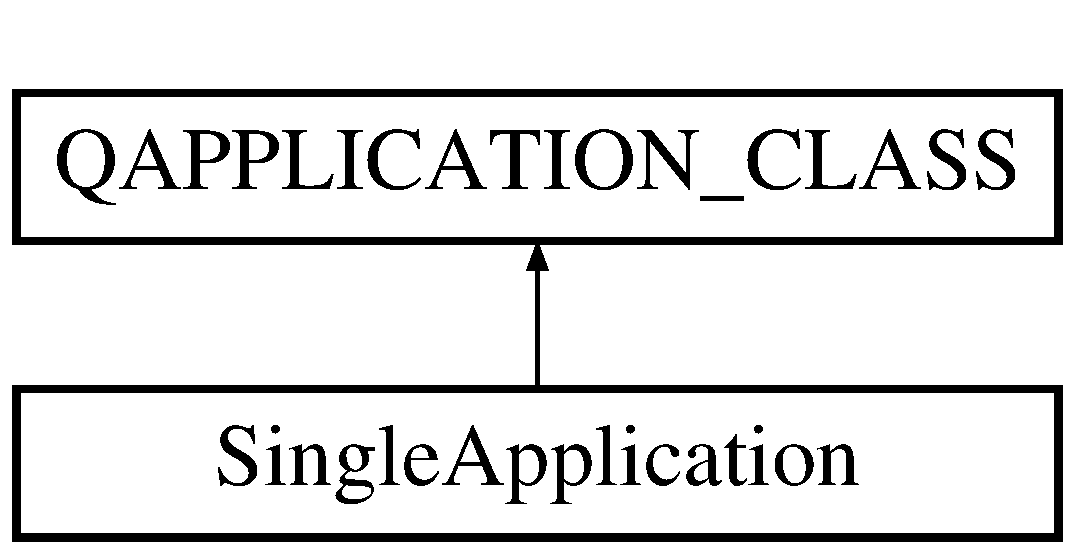
\includegraphics[height=2.000000cm]{class_single_application}
\end{center}
\end{figure}
\subsection*{Signals}
\begin{DoxyCompactItemize}
\item 
\hypertarget{class_single_application_afc6621000a339c859a5f188946505af8}{}void {\bfseries other\+Instance\+Data\+Received} (Q\+Byte\+Array ba)\label{class_single_application_afc6621000a339c859a5f188946505af8}

\end{DoxyCompactItemize}
\subsection*{Public Member Functions}
\begin{DoxyCompactItemize}
\item 
\hyperlink{class_single_application_aa2de0d9769181e267d261f08e3ddc5d9}{Single\+Application} (int \&, char $\ast$\mbox{[}$\,$\mbox{]})
\begin{DoxyCompactList}\small\item\em Constructor. Checks and fires up Local\+Server or closes the program if another instance already exists. \end{DoxyCompactList}\item 
\hypertarget{class_single_application_aa845dd6c6f0b01d8959f4056ded1295b}{}\hyperlink{class_single_application_aa845dd6c6f0b01d8959f4056ded1295b}{$\sim$\+Single\+Application} ()\label{class_single_application_aa845dd6c6f0b01d8959f4056ded1295b}

\begin{DoxyCompactList}\small\item\em Destructor. \end{DoxyCompactList}\end{DoxyCompactItemize}
\subsection*{Private Slots}
\begin{DoxyCompactItemize}
\item 
\hypertarget{class_single_application_a0f048d0c518bd246e3d65760804636a4}{}void \hyperlink{class_single_application_a0f048d0c518bd246e3d65760804636a4}{slot\+Connection\+Established} ()\label{class_single_application_a0f048d0c518bd246e3d65760804636a4}

\begin{DoxyCompactList}\small\item\em Executed when the show\+Up command is sent to Local\+Server. \end{DoxyCompactList}\end{DoxyCompactItemize}
\subsection*{Private Attributes}
\begin{DoxyCompactItemize}
\item 
\hypertarget{class_single_application_ace092941b52064f187862d7be27b7c6a}{}\hyperlink{class_single_application_private}{Single\+Application\+Private} $\ast$ {\bfseries d\+\_\+ptr}\label{class_single_application_ace092941b52064f187862d7be27b7c6a}

\end{DoxyCompactItemize}


\subsection{Constructor \& Destructor Documentation}
\hypertarget{class_single_application_aa2de0d9769181e267d261f08e3ddc5d9}{}\index{Single\+Application@{Single\+Application}!Single\+Application@{Single\+Application}}
\index{Single\+Application@{Single\+Application}!Single\+Application@{Single\+Application}}
\subsubsection[{Single\+Application}]{\setlength{\rightskip}{0pt plus 5cm}Single\+Application\+::\+Single\+Application (
\begin{DoxyParamCaption}
\item[{int \&}]{argc, }
\item[{char $\ast$}]{argv\mbox{[}$\,$\mbox{]}}
\end{DoxyParamCaption}
)\hspace{0.3cm}{\ttfamily [explicit]}}\label{class_single_application_aa2de0d9769181e267d261f08e3ddc5d9}


Constructor. Checks and fires up Local\+Server or closes the program if another instance already exists. 


\begin{DoxyParams}{Parameters}
{\em argc} & \\
\hline
{\em argv} & \\
\hline
\end{DoxyParams}
Garantee thread safe behaviour with a shared memory block

Successful creation means that no main process exists So we start a Local Server to listen for connections

Connect to the Local Server of the main process to notify it that a new process had been started

Even though a shared memory block exists, the original application might have crashed So only after a successful connection is the second instance terminated

Terminate the program using S\+T\+D\+Lib's exit function 

The documentation for this class was generated from the following files\+:\begin{DoxyCompactItemize}
\item 
\hyperlink{singleapplication_8h}{singleapplication.\+h}\item 
\hyperlink{singleapplication_8cpp}{singleapplication.\+cpp}\end{DoxyCompactItemize}

\hypertarget{class_single_application_private}{}\section{Single\+Application\+Private Class Reference}
\label{class_single_application_private}\index{Single\+Application\+Private@{Single\+Application\+Private}}
\subsection*{Public Member Functions}
\begin{DoxyCompactItemize}
\item 
\hypertarget{class_single_application_private_a3bdf4415aaa8f5829e8637f0c75cb697}{}{\bfseries Single\+Application\+Private} (\hyperlink{class_single_application}{Single\+Application} $\ast$q\+\_\+ptr)\label{class_single_application_private_a3bdf4415aaa8f5829e8637f0c75cb697}

\item 
void \hyperlink{class_single_application_private_a4d7284bd84a7a08aeaa90c7c350bb1cd}{start\+Server} (Q\+String \&server\+Name)
\end{DoxyCompactItemize}
\subsection*{Public Attributes}
\begin{DoxyCompactItemize}
\item 
\hypertarget{class_single_application_private_a68209c957c6bf79051354a8ecf4a6b49}{}Q\+Shared\+Memory $\ast$ {\bfseries memory}\label{class_single_application_private_a68209c957c6bf79051354a8ecf4a6b49}

\item 
\hypertarget{class_single_application_private_aeace2f08f4ed4642b4a5f7c4408a14f2}{}\hyperlink{class_single_application}{Single\+Application} $\ast$ {\bfseries q\+\_\+ptr}\label{class_single_application_private_aeace2f08f4ed4642b4a5f7c4408a14f2}

\item 
\hypertarget{class_single_application_private_ae95f6462bd243b08cdff4815d671a21f}{}Q\+Local\+Server $\ast$ {\bfseries server}\label{class_single_application_private_ae95f6462bd243b08cdff4815d671a21f}

\item 
\hypertarget{class_single_application_private_a4557ba81fb05cf961cb2285b889c7fff}{}Q\+Local\+Socket $\ast$ {\bfseries socket}\label{class_single_application_private_a4557ba81fb05cf961cb2285b889c7fff}

\end{DoxyCompactItemize}


\subsection{Member Function Documentation}
\hypertarget{class_single_application_private_a4d7284bd84a7a08aeaa90c7c350bb1cd}{}\index{Single\+Application\+Private@{Single\+Application\+Private}!start\+Server@{start\+Server}}
\index{start\+Server@{start\+Server}!Single\+Application\+Private@{Single\+Application\+Private}}
\subsubsection[{start\+Server}]{\setlength{\rightskip}{0pt plus 5cm}void Single\+Application\+Private\+::start\+Server (
\begin{DoxyParamCaption}
\item[{Q\+String \&}]{server\+Name}
\end{DoxyParamCaption}
)\hspace{0.3cm}{\ttfamily [inline]}}\label{class_single_application_private_a4d7284bd84a7a08aeaa90c7c350bb1cd}
Start a Q\+Local\+Server to listen for connections 

The documentation for this class was generated from the following file\+:\begin{DoxyCompactItemize}
\item 
\hyperlink{singleapplication_8cpp}{singleapplication.\+cpp}\end{DoxyCompactItemize}

\hypertarget{class_tab}{}\section{Tab Class Reference}
\label{class_tab}\index{Tab@{Tab}}


U\+N\+K\+N\+O\+W\+N.  




{\ttfamily \#include $<$tab.\+h$>$}

Inheritance diagram for Tab\+:\begin{figure}[H]
\begin{center}
\leavevmode
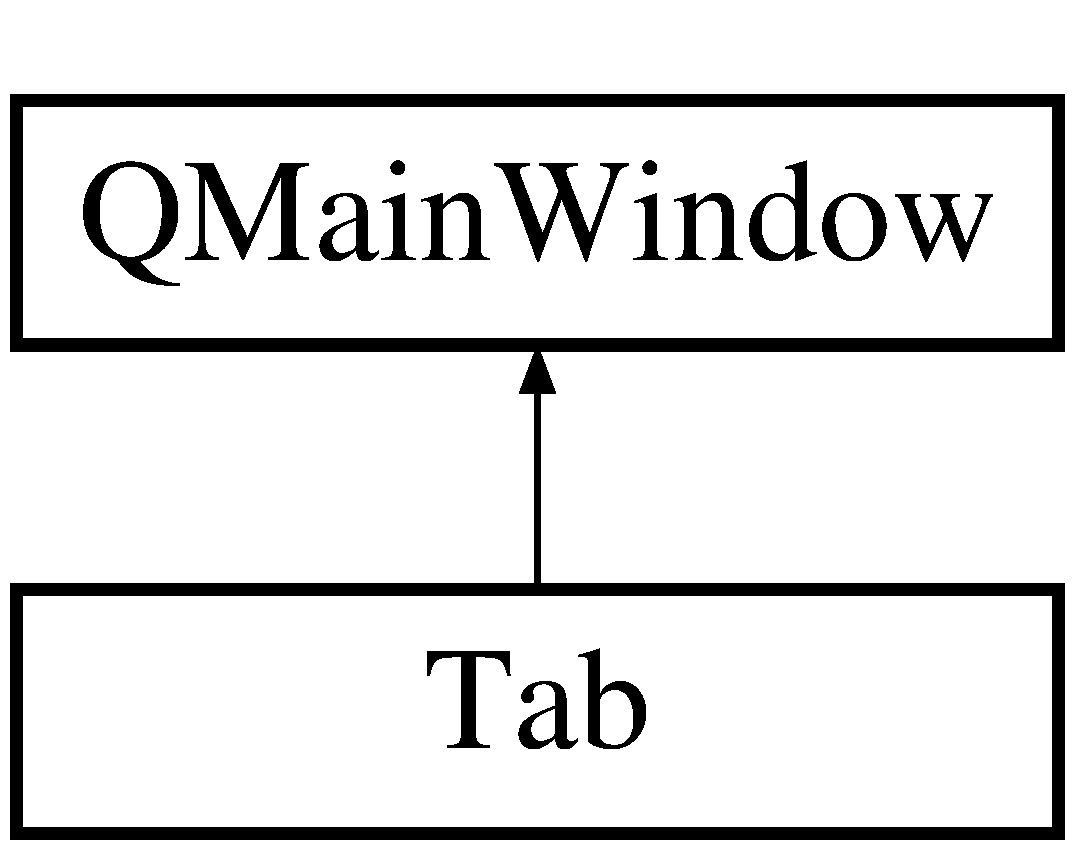
\includegraphics[height=2.000000cm]{class_tab}
\end{center}
\end{figure}
\subsection*{Public Member Functions}
\begin{DoxyCompactItemize}
\item 
\hyperlink{class_tab_a3e967f9ec671509bfab71e919c838876}{Tab} (Q\+Widget $\ast$parent=0)
\begin{DoxyCompactList}\small\item\em U\+N\+K\+N\+O\+W\+N. \end{DoxyCompactList}\item 
virtual \hyperlink{class_tab_a8cc210bcede02daa21145bb1675c3c80}{$\sim$\+Tab} ()
\begin{DoxyCompactList}\small\item\em Destructor for the \hyperlink{class_tab}{Tab} objects. \end{DoxyCompactList}\item 
\hypertarget{class_tab_a28ed89a733484410df7455110425c50d}{}Q\+Text\+Document $\ast$ {\bfseries get\+Code\+Document} ()\label{class_tab_a28ed89a733484410df7455110425c50d}

\item 
\hypertarget{class_tab_aff2b75621d226d4941670b66450c574b}{}void {\bfseries save\+Code\+To\+File} (const Q\+String \&file\+Path, \hyperlink{class_assembler}{Assembler} $\ast$assembler, bool change\+Code\+Modified\+Flag=true, bool debug\+Mode=false)\label{class_tab_aff2b75621d226d4941670b66450c574b}

\item 
\hypertarget{class_tab_a26b069ece03c8df2fe26a98bc5c0f985}{}void {\bfseries save\+Input\+To\+File} (const Q\+String \&file\+Path)\label{class_tab_a26b069ece03c8df2fe26a98bc5c0f985}

\item 
\hypertarget{class_tab_afc158a43658eba563e286bc8385745da}{}void {\bfseries load\+Output\+From\+File} (const Q\+String \&file\+Path)\label{class_tab_afc158a43658eba563e286bc8385745da}

\item 
\hypertarget{class_tab_a8e95ad5c45974adfe3f2c76a370c5364}{}void {\bfseries load\+Code\+From\+File} (const Q\+String \&file\+Path)\label{class_tab_a8e95ad5c45974adfe3f2c76a370c5364}

\item 
void \hyperlink{class_tab_af4c53acabb77314b325490e7895c4bfb}{append\+Output} (Q\+String msg)
\item 
\hypertarget{class_tab_a3a7e86d4a00ee457caa53c56f2fb7595}{}Q\+String {\bfseries get\+Current\+File\+Path} ()\label{class_tab_a3a7e86d4a00ee457caa53c56f2fb7595}

\item 
\hypertarget{class_tab_a94288e7eebc73fa8c48611ea59afec24}{}void {\bfseries clear\+Output} ()\label{class_tab_a94288e7eebc73fa8c48611ea59afec24}

\item 
\hypertarget{class_tab_a4e545dbb1b91938197393089766202d1}{}void {\bfseries set\+Fonts} ()\label{class_tab_a4e545dbb1b91938197393089766202d1}

\end{DoxyCompactItemize}
\subsection*{Public Attributes}
\begin{DoxyCompactItemize}
\item 
\hypertarget{class_tab_a2ca89e986540f7ad32fd78712ed078ec}{}\hyperlink{class_code_editor}{Code\+Editor} $\ast$ {\bfseries code}\label{class_tab_a2ca89e986540f7ad32fd78712ed078ec}

\end{DoxyCompactItemize}
\subsection*{Private Attributes}
\begin{DoxyCompactItemize}
\item 
\hypertarget{class_tab_a177d0ededc7732e0eb9f4ab3946a0613}{}Q\+V\+Box\+Layout $\ast$ \hyperlink{class_tab_a177d0ededc7732e0eb9f4ab3946a0613}{input\+Layout}\label{class_tab_a177d0ededc7732e0eb9f4ab3946a0613}

\begin{DoxyCompactList}\small\item\em Text fields. \end{DoxyCompactList}\item 
\hypertarget{class_tab_a2022402e6791f8706264ead579db8ddb}{}Q\+V\+Box\+Layout $\ast$ {\bfseries output\+Layout}\label{class_tab_a2022402e6791f8706264ead579db8ddb}

\item 
\hypertarget{class_tab_a0b1098aee5962a413385026bb97217ad}{}\hyperlink{class_ru_q_text_edit}{Ru\+Q\+Text\+Edit} $\ast$ {\bfseries input}\label{class_tab_a0b1098aee5962a413385026bb97217ad}

\item 
\hypertarget{class_tab_a487419863e6026db90ecdeb1e312e98d}{}\hyperlink{class_ru_q_text_edit}{Ru\+Q\+Text\+Edit} $\ast$ {\bfseries output}\label{class_tab_a487419863e6026db90ecdeb1e312e98d}

\item 
\hypertarget{class_tab_a9035df5e25ea1c063800729c208899da}{}Q\+Widget $\ast$ {\bfseries input\+Widget}\label{class_tab_a9035df5e25ea1c063800729c208899da}

\item 
\hypertarget{class_tab_ac9e36aa86c10d2222c7c64146e8ccdc4}{}Q\+Widget $\ast$ {\bfseries output\+Widget}\label{class_tab_ac9e36aa86c10d2222c7c64146e8ccdc4}

\item 
\hypertarget{class_tab_a2fcfb7fc3caf22a3e024efde604385b4}{}Q\+String {\bfseries current\+File\+Path}\label{class_tab_a2fcfb7fc3caf22a3e024efde604385b4}

\end{DoxyCompactItemize}


\subsection{Detailed Description}
U\+N\+K\+N\+O\+W\+N. 

U\+N\+K\+N\+O\+W\+N 

\subsection{Constructor \& Destructor Documentation}
\hypertarget{class_tab_a3e967f9ec671509bfab71e919c838876}{}\index{Tab@{Tab}!Tab@{Tab}}
\index{Tab@{Tab}!Tab@{Tab}}
\subsubsection[{Tab}]{\setlength{\rightskip}{0pt plus 5cm}Tab\+::\+Tab (
\begin{DoxyParamCaption}
\item[{Q\+Widget $\ast$}]{parent = {\ttfamily 0}}
\end{DoxyParamCaption}
)\hspace{0.3cm}{\ttfamily [explicit]}}\label{class_tab_a3e967f9ec671509bfab71e919c838876}


U\+N\+K\+N\+O\+W\+N. 

Setting code field

Setting input and output fields

Setting io and code fonts

Restore state \hypertarget{class_tab_a8cc210bcede02daa21145bb1675c3c80}{}\index{Tab@{Tab}!````~Tab@{$\sim$\+Tab}}
\index{````~Tab@{$\sim$\+Tab}!Tab@{Tab}}
\subsubsection[{$\sim$\+Tab}]{\setlength{\rightskip}{0pt plus 5cm}Tab\+::$\sim$\+Tab (
\begin{DoxyParamCaption}
{}
\end{DoxyParamCaption}
)\hspace{0.3cm}{\ttfamily [virtual]}}\label{class_tab_a8cc210bcede02daa21145bb1675c3c80}


Destructor for the \hyperlink{class_tab}{Tab} objects. 



\subsection{Member Function Documentation}
\hypertarget{class_tab_af4c53acabb77314b325490e7895c4bfb}{}\index{Tab@{Tab}!append\+Output@{append\+Output}}
\index{append\+Output@{append\+Output}!Tab@{Tab}}
\subsubsection[{append\+Output}]{\setlength{\rightskip}{0pt plus 5cm}void Tab\+::append\+Output (
\begin{DoxyParamCaption}
\item[{Q\+String}]{msg}
\end{DoxyParamCaption}
)}\label{class_tab_af4c53acabb77314b325490e7895c4bfb}
Scroll 

The documentation for this class was generated from the following files\+:\begin{DoxyCompactItemize}
\item 
\hyperlink{tab_8h}{tab.\+h}\item 
\hyperlink{tab_8cpp}{tab.\+cpp}\end{DoxyCompactItemize}

\hypertarget{struct_ru_q_plain_text_edit_1_1_watch}{}\section{Ru\+Q\+Plain\+Text\+Edit\+:\+:Watch Struct Reference}
\label{struct_ru_q_plain_text_edit_1_1_watch}\index{Ru\+Q\+Plain\+Text\+Edit\+::\+Watch@{Ru\+Q\+Plain\+Text\+Edit\+::\+Watch}}


Defines a structure to keep track of a watched variable.  




{\ttfamily \#include $<$ruqplaintextedit.\+h$>$}

\subsection*{Public Attributes}
\begin{DoxyCompactItemize}
\item 
\hypertarget{struct_ru_q_plain_text_edit_1_1_watch_a1be872e72e8414ba1efa6a36738914e3}{}Q\+String {\bfseries name}\label{struct_ru_q_plain_text_edit_1_1_watch_a1be872e72e8414ba1efa6a36738914e3}

\item 
\hypertarget{struct_ru_q_plain_text_edit_1_1_watch_a9ba866a2946627df2dc301bb7eb1279a}{}int {\bfseries type}\label{struct_ru_q_plain_text_edit_1_1_watch_a9ba866a2946627df2dc301bb7eb1279a}

\item 
\hypertarget{struct_ru_q_plain_text_edit_1_1_watch_a1bf8cee83d981ae218097934125f5ef0}{}int {\bfseries size}\label{struct_ru_q_plain_text_edit_1_1_watch_a1bf8cee83d981ae218097934125f5ef0}

\item 
\hypertarget{struct_ru_q_plain_text_edit_1_1_watch_a092b03dbdf3af5c7dcfd12940c19a1c3}{}int {\bfseries array\+Size}\label{struct_ru_q_plain_text_edit_1_1_watch_a092b03dbdf3af5c7dcfd12940c19a1c3}

\item 
\hypertarget{struct_ru_q_plain_text_edit_1_1_watch_a8a69b8fd93364e59cb025dac18cadc64}{}bool {\bfseries address}\label{struct_ru_q_plain_text_edit_1_1_watch_a8a69b8fd93364e59cb025dac18cadc64}

\end{DoxyCompactItemize}


\subsection{Detailed Description}
Defines a structure to keep track of a watched variable. 

The documentation for this struct was generated from the following file\+:\begin{DoxyCompactItemize}
\item 
\hyperlink{ruqplaintextedit_8h}{ruqplaintextedit.\+h}\end{DoxyCompactItemize}

\hypertarget{class_watch_settins_widget}{}\section{Watch\+Settins\+Widget Class Reference}
\label{class_watch_settins_widget}\index{Watch\+Settins\+Widget@{Watch\+Settins\+Widget}}
Inheritance diagram for Watch\+Settins\+Widget\+:\begin{figure}[H]
\begin{center}
\leavevmode
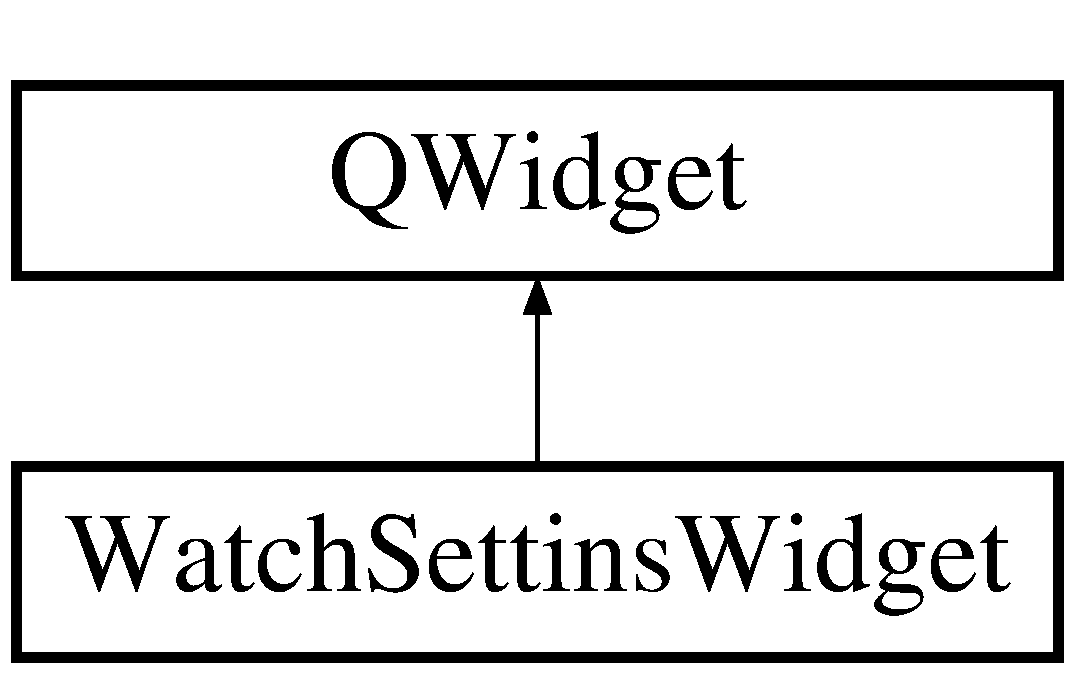
\includegraphics[height=2.000000cm]{class_watch_settins_widget}
\end{center}
\end{figure}
\subsection*{Signals}
\begin{DoxyCompactItemize}
\item 
\hypertarget{class_watch_settins_widget_aa8795e2002112890a4d579e99bc5cd87}{}void {\bfseries settings\+Changed} (void)\label{class_watch_settins_widget_aa8795e2002112890a4d579e99bc5cd87}

\end{DoxyCompactItemize}
\subsection*{Public Member Functions}
\begin{DoxyCompactItemize}
\item 
\hyperlink{class_watch_settins_widget_a6a84d2b11a68201f1a035587757d8fc5}{Watch\+Settins\+Widget} (Q\+Widget $\ast$parent=0)
\begin{DoxyCompactList}\small\item\em This defines the layout such as spacing and items of the variable watch area. \end{DoxyCompactList}\item 
\hypertarget{class_watch_settins_widget_a1d32e0025eb6328e829561fc6b9d62c1}{}int {\bfseries sum\+Size} ()\label{class_watch_settins_widget_a1d32e0025eb6328e829561fc6b9d62c1}

\item 
\hypertarget{class_watch_settins_widget_ae3057ad6e1835532b01be44f0ee02a1f}{}Q\+Size {\bfseries size\+Hint} () const \label{class_watch_settins_widget_ae3057ad6e1835532b01be44f0ee02a1f}

\end{DoxyCompactItemize}
\subsection*{Public Attributes}
\begin{DoxyCompactItemize}
\item 
\hypertarget{class_watch_settins_widget_a8922245dfda45811c2efd34c9502c6be}{}Q\+Combo\+Box $\ast$ {\bfseries type\+Combo\+Box}\label{class_watch_settins_widget_a8922245dfda45811c2efd34c9502c6be}

\item 
\hypertarget{class_watch_settins_widget_a7a22d14236236072644d6cb36dabf12b}{}Q\+Combo\+Box $\ast$ {\bfseries size\+Combo\+Box}\label{class_watch_settins_widget_a7a22d14236236072644d6cb36dabf12b}

\item 
\hypertarget{class_watch_settins_widget_a7d7a33acd1841ae2c4e8e70eda14c5fb}{}Q\+Line\+Edit $\ast$ {\bfseries array\+Size\+Edit}\label{class_watch_settins_widget_a7d7a33acd1841ae2c4e8e70eda14c5fb}

\item 
\hypertarget{class_watch_settins_widget_a057d81b10a5d0ac66e9a3c3aab6c1f72}{}Q\+Check\+Box $\ast$ {\bfseries address\+Checkbox}\label{class_watch_settins_widget_a057d81b10a5d0ac66e9a3c3aab6c1f72}

\end{DoxyCompactItemize}
\subsection*{Private Attributes}
\begin{DoxyCompactItemize}
\item 
\hypertarget{class_watch_settins_widget_acdbd67294d078bc130a6612c69ae56a5}{}Q\+H\+Box\+Layout $\ast$ {\bfseries layout}\label{class_watch_settins_widget_acdbd67294d078bc130a6612c69ae56a5}

\end{DoxyCompactItemize}


\subsection{Constructor \& Destructor Documentation}
\hypertarget{class_watch_settins_widget_a6a84d2b11a68201f1a035587757d8fc5}{}\index{Watch\+Settins\+Widget@{Watch\+Settins\+Widget}!Watch\+Settins\+Widget@{Watch\+Settins\+Widget}}
\index{Watch\+Settins\+Widget@{Watch\+Settins\+Widget}!Watch\+Settins\+Widget@{Watch\+Settins\+Widget}}
\subsubsection[{Watch\+Settins\+Widget}]{\setlength{\rightskip}{0pt plus 5cm}Watch\+Settins\+Widget\+::\+Watch\+Settins\+Widget (
\begin{DoxyParamCaption}
\item[{Q\+Widget $\ast$}]{parent = {\ttfamily 0}}
\end{DoxyParamCaption}
)\hspace{0.3cm}{\ttfamily [explicit]}}\label{class_watch_settins_widget_a6a84d2b11a68201f1a035587757d8fc5}


This defines the layout such as spacing and items of the variable watch area. 

First, the parent widget is passed to the class. Next, the form items are added and spaced appropriately. The form items are then further defined and then connected. 

The documentation for this class was generated from the following files\+:\begin{DoxyCompactItemize}
\item 
watchsettinswidget.\+h\item 
\hyperlink{watchsettinswidget_8cpp}{watchsettinswidget.\+cpp}\end{DoxyCompactItemize}

\chapter{File Documentation}
\hypertarget{assembler_8cpp}{}\section{assembler.\+cpp File Reference}
\label{assembler_8cpp}\index{assembler.\+cpp@{assembler.\+cpp}}
{\ttfamily \#include \char`\"{}assembler.\+h\char`\"{}}\\*


\subsection{Detailed Description}
Impliments the Assmbler class 
\hypertarget{assembler_8h}{}\section{assembler.\+h File Reference}
\label{assembler_8h}\index{assembler.\+h@{assembler.\+h}}
{\ttfamily \#include $<$Q\+Object$>$}\\*
{\ttfamily \#include $<$Q\+Map$>$}\\*
{\ttfamily \#include $<$Q\+List$>$}\\*
{\ttfamily \#include $<$Q\+Reg\+Exp$>$}\\*
{\ttfamily \#include $<$Q\+File$>$}\\*
{\ttfamily \#include $<$Q\+Text\+Stream$>$}\\*
{\ttfamily \#include $<$Q\+Vector$>$}\\*
{\ttfamily \#include $<$Q\+Text\+Char\+Format$>$}\\*
{\ttfamily \#include $<$Q\+Settings$>$}\\*
{\ttfamily \#include $<$Q\+Palette$>$}\\*
{\ttfamily \#include \char`\"{}common.\+h\char`\"{}}\\*
{\ttfamily \#include \char`\"{}codeeditor.\+h\char`\"{}}\\*
\subsection*{Classes}
\begin{DoxyCompactItemize}
\item 
class \hyperlink{class_assembler}{Assembler}
\begin{DoxyCompactList}\small\item\em This is the base class that all assemblers inherit. \end{DoxyCompactList}\item 
struct \hyperlink{struct_assembler_1_1_line_num}{Assembler\+::\+Line\+Num}
\item 
struct \hyperlink{struct_assembler_1_1_highlighting_rule}{Assembler\+::\+Highlighting\+Rule}
\end{DoxyCompactItemize}


\subsection{Detailed Description}
Base class for creating assembler instances 
\hypertarget{codeeditor_8cpp}{}\section{codeeditor.\+cpp File Reference}
\label{codeeditor_8cpp}\index{codeeditor.\+cpp@{codeeditor.\+cpp}}
{\ttfamily \#include \char`\"{}codeeditor.\+h\char`\"{}}\\*


\subsection{Detailed Description}
Impliments the code editing area 
\hypertarget{codeeditor_8h}{}\section{codeeditor.\+h File Reference}
\label{codeeditor_8h}\index{codeeditor.\+h@{codeeditor.\+h}}
{\ttfamily \#include $<$Q\+Painter$>$}\\*
{\ttfamily \#include $<$Q\+Text\+Block$>$}\\*
{\ttfamily \#include $<$Q\+Scroll\+Bar$>$}\\*
{\ttfamily \#include $<$Q\+Drag\+Enter\+Event$>$}\\*
{\ttfamily \#include $<$Q\+Drop\+Event$>$}\\*
{\ttfamily \#include $<$Q\+Mime\+Data$>$}\\*
{\ttfamily \#include \char`\"{}ruqplaintextedit.\+h\char`\"{}}\\*
{\ttfamily \#include $<$Q\+Url$>$}\\*
\subsection*{Classes}
\begin{DoxyCompactItemize}
\item 
class \hyperlink{class_code_editor}{Code\+Editor}
\item 
class \hyperlink{class_line_number_area}{Line\+Number\+Area}
\end{DoxyCompactItemize}


\subsection{Detailed Description}
Contains definitions for objects pertaining to the code editing section 
\hypertarget{common_8cpp}{}\section{common.\+cpp File Reference}
\label{common_8cpp}\index{common.\+cpp@{common.\+cpp}}
{\ttfamily \#include \char`\"{}common.\+h\char`\"{}}\\*


\subsection{Detailed Description}
U\+N\+K\+N\+O\+W\+N 
\hypertarget{common_8h}{}\section{common.\+h File Reference}
\label{common_8h}\index{common.\+h@{common.\+h}}
{\ttfamily \#include $<$Q\+String$>$}\\*
{\ttfamily \#include $<$Q\+Core\+Application$>$}\\*
{\ttfamily \#include $<$Q\+File$>$}\\*
{\ttfamily \#include $<$Q\+Dir$>$}\\*
\subsection*{Functions}
\begin{DoxyCompactItemize}
\item 
\hypertarget{namespace_common_ab2131edad5b444e7cdf2d487035acfb8}{}Q\+String {\bfseries Common\+::application\+Data\+Path} ()\label{namespace_common_ab2131edad5b444e7cdf2d487035acfb8}

\item 
\hypertarget{namespace_common_ad6dcc120315bccbb162820cfdd301bee}{}Q\+String {\bfseries Common\+::path\+In\+Temp} (Q\+String path)\label{namespace_common_ad6dcc120315bccbb162820cfdd301bee}

\end{DoxyCompactItemize}


\subsection{Detailed Description}
Base U\+N\+K\+N\+O\+W\+N 
\hypertarget{debuganycommandwidget_8cpp}{}\section{debuganycommandwidget.\+cpp File Reference}
\label{debuganycommandwidget_8cpp}\index{debuganycommandwidget.\+cpp@{debuganycommandwidget.\+cpp}}
{\ttfamily \#include \char`\"{}debuganycommandwidget.\+h\char`\"{}}\\*


\subsection{Detailed Description}
Impliments the debugger's stepping features 
\hypertarget{debuganycommandwidget_8h}{}\section{debuganycommandwidget.\+h File Reference}
\label{debuganycommandwidget_8h}\index{debuganycommandwidget.\+h@{debuganycommandwidget.\+h}}
{\ttfamily \#include $<$Q\+Widget$>$}\\*
{\ttfamily \#include $<$Q\+Label$>$}\\*
{\ttfamily \#include $<$Q\+Line\+Edit$>$}\\*
{\ttfamily \#include $<$Q\+Push\+Button$>$}\\*
{\ttfamily \#include $<$Q\+H\+Box\+Layout$>$}\\*
{\ttfamily \#include $<$Q\+Key\+Event$>$}\\*
{\ttfamily \#include $<$Q\+Check\+Box$>$}\\*
\subsection*{Classes}
\begin{DoxyCompactItemize}
\item 
class \hyperlink{class_debug_any_command_widget}{Debug\+Any\+Command\+Widget}
\begin{DoxyCompactList}\small\item\em This class does...... \end{DoxyCompactList}\end{DoxyCompactItemize}


\subsection{Detailed Description}
U\+N\+K\+N\+O\+W\+N 
\hypertarget{debugger_8cpp}{}\section{debugger.\+cpp File Reference}
\label{debugger_8cpp}\index{debugger.\+cpp@{debugger.\+cpp}}
{\ttfamily \#include \char`\"{}debugger.\+h\char`\"{}}\\*


\subsection{Detailed Description}
Sets debugger information and runs the debugger. 
\hypertarget{debugger_8h}{}\section{debugger.\+h File Reference}
\label{debugger_8h}\index{debugger.\+h@{debugger.\+h}}
{\ttfamily \#include $<$Q\+Process$>$}\\*
{\ttfamily \#include $<$Q\+Process\+Environment$>$}\\*
{\ttfamily \#include $<$Q\+String$>$}\\*
{\ttfamily \#include $<$Q\+Text\+Stream$>$}\\*
{\ttfamily \#include $<$Q\+Text\+Edit$>$}\\*
{\ttfamily \#include $<$Q\+File$>$}\\*
{\ttfamily \#include $<$Q\+Vector$>$}\\*
{\ttfamily \#include $<$Q\+Core\+Application$>$}\\*
{\ttfamily \#include $<$Q\+Timer$>$}\\*
{\ttfamily \#include $<$Q\+Queue$>$}\\*
{\ttfamily \#include $<$Q\+Settings$>$}\\*
{\ttfamily \#include \char`\"{}assembler.\+h\char`\"{}}\\*
{\ttfamily \#include $<$signal.\+h$>$}\\*
\subsection*{Classes}
\begin{DoxyCompactItemize}
\item 
class \hyperlink{class_debugger}{Debugger}
\begin{DoxyCompactList}\small\item\em This class represents the debugger. \end{DoxyCompactList}\item 
struct \hyperlink{struct_debugger_1_1registers_info}{Debugger\+::registers\+Info}
\item 
struct \hyperlink{struct_debugger_1_1memory_info}{Debugger\+::memory\+Info}
\end{DoxyCompactItemize}
\subsection*{Enumerations}
\begin{DoxyCompactItemize}
\item 
\hypertarget{debugger_8h_a4d452a0b8b1cbbea4f29aac39d4aa529}{}enum {\bfseries Debug\+Action\+Type} \{ \\*
{\bfseries ni}, 
{\bfseries si}, 
{\bfseries show\+Line}, 
{\bfseries info\+Registers}, 
\\*
{\bfseries info\+Memory}, 
{\bfseries any\+Action}, 
{\bfseries none}, 
{\bfseries breakpoint}
 \}\label{debugger_8h_a4d452a0b8b1cbbea4f29aac39d4aa529}

\end{DoxyCompactItemize}


\subsection{Detailed Description}
Defines the debugger. 
\hypertarget{debugtablewidget_8cpp}{}\section{debugtablewidget.\+cpp File Reference}
\label{debugtablewidget_8cpp}\index{debugtablewidget.\+cpp@{debugtablewidget.\+cpp}}
{\ttfamily \#include \char`\"{}debugtablewidget.\+h\char`\"{}}\\*


\subsection{Detailed Description}
Impliments the debuging memory window 
\hypertarget{debugtablewidget_8h}{}\section{debugtablewidget.\+h File Reference}
\label{debugtablewidget_8h}\index{debugtablewidget.\+h@{debugtablewidget.\+h}}
{\ttfamily \#include $<$Q\+Table\+Widget$>$}\\*
{\ttfamily \#include $<$Q\+Desktop\+Widget$>$}\\*
{\ttfamily \#include $<$Q\+Header\+View$>$}\\*
{\ttfamily \#include $<$Q\+Mouse\+Event$>$}\\*
{\ttfamily \#include $<$Q\+Action$>$}\\*
{\ttfamily \#include $<$Q\+Menu$>$}\\*
{\ttfamily \#include $<$Q\+Byte\+Array$>$}\\*
{\ttfamily \#include \char`\"{}debugger.\+h\char`\"{}}\\*
{\ttfamily \#include \char`\"{}watchsettinswidget.\+h\char`\"{}}\\*
{\ttfamily \#include \char`\"{}ruqplaintextedit.\+h\char`\"{}}\\*
\subsection*{Classes}
\begin{DoxyCompactItemize}
\item 
class \hyperlink{class_debug_table_widget}{Debug\+Table\+Widget}
\begin{DoxyCompactList}\small\item\em This class represents the Memory table. \end{DoxyCompactList}\end{DoxyCompactItemize}
\subsection*{Enumerations}
\begin{DoxyCompactItemize}
\item 
\hypertarget{debugtablewidget_8h_a351fb1d60db94ff69e3bafa1b11806a9}{}enum {\bfseries Debug\+Table\+Widget\+Type} \{ {\bfseries registers\+Table}, 
{\bfseries memory\+Table}
 \}\label{debugtablewidget_8h_a351fb1d60db94ff69e3bafa1b11806a9}

\end{DoxyCompactItemize}


\subsection{Detailed Description}
Defines the debugging window which the user interfaces with it. 
\hypertarget{fasm_8cpp}{}\section{fasm.\+cpp File Reference}
\label{fasm_8cpp}\index{fasm.\+cpp@{fasm.\+cpp}}
{\ttfamily \#include \char`\"{}fasm.\+h\char`\"{}}\\*


\subsection{Detailed Description}
Impliments the \hyperlink{class_f_a_s_m}{F\+A\+S\+M} assembler 
\hypertarget{fasm_8h}{}\section{fasm.\+h File Reference}
\label{fasm_8h}\index{fasm.\+h@{fasm.\+h}}
{\ttfamily \#include $<$Q\+Process$>$}\\*
{\ttfamily \#include $<$Q\+Linked\+List$>$}\\*
{\ttfamily \#include \char`\"{}assembler.\+h\char`\"{}}\\*
\subsection*{Classes}
\begin{DoxyCompactItemize}
\item 
class \hyperlink{class_f_a_s_m}{F\+A\+S\+M}
\begin{DoxyCompactList}\small\item\em This class defines the behavior for the \hyperlink{class_f_a_s_m}{F\+A\+S\+M} assembler. \end{DoxyCompactList}\end{DoxyCompactItemize}


\subsection{Detailed Description}
Defines the \hyperlink{class_f_a_s_m}{F\+A\+S\+M} assembler 
\hypertarget{finddialog_8cpp}{}\section{finddialog.\+cpp File Reference}
\label{finddialog_8cpp}\index{finddialog.\+cpp@{finddialog.\+cpp}}
{\ttfamily \#include \char`\"{}finddialog.\+h\char`\"{}}\\*


\subsection{Detailed Description}
Impliments the find text widget. 
\hypertarget{finddialog_8h}{}\section{finddialog.\+h File Reference}
\label{finddialog_8h}\index{finddialog.\+h@{finddialog.\+h}}
{\ttfamily \#include $<$Q\+Widget$>$}\\*
{\ttfamily \#include $<$Q\+Check\+Box$>$}\\*
{\ttfamily \#include $<$Q\+Label$>$}\\*
{\ttfamily \#include $<$Q\+Line\+Edit$>$}\\*
{\ttfamily \#include $<$Q\+Push\+Button$>$}\\*
{\ttfamily \#include $<$Q\+H\+Box\+Layout$>$}\\*
{\ttfamily \#include $<$Q\+V\+Box\+Layout$>$}\\*
{\ttfamily \#include $<$Q\+Close\+Event$>$}\\*
\subsection*{Classes}
\begin{DoxyCompactItemize}
\item 
class \hyperlink{class_find_dialog}{Find\+Dialog}
\begin{DoxyCompactList}\small\item\em This class represents the \char`\"{}find text\char`\"{} functionality. \end{DoxyCompactList}\end{DoxyCompactItemize}


\subsection{Detailed Description}
The dialog box used to find text. 
\hypertarget{gas_8cpp}{}\section{gas.\+cpp File Reference}
\label{gas_8cpp}\index{gas.\+cpp@{gas.\+cpp}}
{\ttfamily \#include \char`\"{}gas.\+h\char`\"{}}\\*


\subsection{Detailed Description}
Impliments the \hyperlink{class_g_a_s}{G\+A\+S} assembler. 
\hypertarget{gas_8h}{}\section{gas.\+h File Reference}
\label{gas_8h}\index{gas.\+h@{gas.\+h}}
{\ttfamily \#include \char`\"{}assembler.\+h\char`\"{}}\\*
\subsection*{Classes}
\begin{DoxyCompactItemize}
\item 
class \hyperlink{class_g_a_s}{G\+A\+S}
\begin{DoxyCompactList}\small\item\em This class defines the behavior for the \hyperlink{class_g_a_s}{G\+A\+S} assembler. \end{DoxyCompactList}\end{DoxyCompactItemize}


\subsection{Detailed Description}
Defines the \hyperlink{class_g_a_s}{G\+A\+S} assembler. 
\hypertarget{getstartedwidget_8cpp}{}\section{getstartedwidget.\+cpp File Reference}
\label{getstartedwidget_8cpp}\index{getstartedwidget.\+cpp@{getstartedwidget.\+cpp}}
{\ttfamily \#include \char`\"{}getstartedwidget.\+h\char`\"{}}\\*


\subsection{Detailed Description}
Impliments the opening window. 
\hypertarget{getstartedwidget_8h}{}\section{getstartedwidget.\+h File Reference}
\label{getstartedwidget_8h}\index{getstartedwidget.\+h@{getstartedwidget.\+h}}
{\ttfamily \#include $<$Q\+V\+Box\+Layout$>$}\\*
{\ttfamily \#include $<$Q\+Command\+Link\+Button$>$}\\*
{\ttfamily \#include $<$Q\+Label$>$}\\*
{\ttfamily \#include $<$Q\+Spacer\+Item$>$}\\*
\subsection*{Classes}
\begin{DoxyCompactItemize}
\item 
class \hyperlink{class_get_started_widget}{Get\+Started\+Widget}
\end{DoxyCompactItemize}


\subsection{Detailed Description}
Defines the enry window. 
\hypertarget{highlighter_8cpp}{}\section{highlighter.\+cpp File Reference}
\label{highlighter_8cpp}\index{highlighter.\+cpp@{highlighter.\+cpp}}
{\ttfamily \#include \char`\"{}highlighter.\+h\char`\"{}}\\*


\subsection{Detailed Description}
The code highlighting features are defined here. 
\hypertarget{highlighter_8h}{}\section{highlighter.\+h File Reference}
\label{highlighter_8h}\index{highlighter.\+h@{highlighter.\+h}}
{\ttfamily \#include $<$Q\+Syntax\+Highlighter$>$}\\*
{\ttfamily \#include $<$Q\+Settings$>$}\\*
{\ttfamily \#include $<$Q\+Palette$>$}\\*
{\ttfamily \#include $<$Q\+Text\+Document$>$}\\*
{\ttfamily \#include \char`\"{}assembler.\+h\char`\"{}}\\*
\subsection*{Classes}
\begin{DoxyCompactItemize}
\item 
class \hyperlink{class_highlighter}{Highlighter}
\begin{DoxyCompactList}\small\item\em This class defines the rules of syntax highlighting. \end{DoxyCompactList}\end{DoxyCompactItemize}


\subsection{Detailed Description}
Defines the highlighting class. 
\hypertarget{main_8cpp}{}\section{main.\+cpp File Reference}
\label{main_8cpp}\index{main.\+cpp@{main.\+cpp}}
{\ttfamily \#include \char`\"{}mainwindow.\+h\char`\"{}}\\*
{\ttfamily \#include $<$Q\+Application$>$}\\*
{\ttfamily \#include $<$Q\+Translator$>$}\\*
{\ttfamily \#include $<$Q\+Text\+Codec$>$}\\*
{\ttfamily \#include $<$Q\+Settings$>$}\\*
{\ttfamily \#include $<$Q\+Push\+Button$>$}\\*
{\ttfamily \#include $<$Q\+Object$>$}\\*
{\ttfamily \#include \char`\"{}singleapplication.\+h\char`\"{}}\\*
\subsection*{Functions}
\begin{DoxyCompactItemize}
\item 
\hypertarget{main_8cpp_a0ddf1224851353fc92bfbff6f499fa97}{}int {\bfseries main} (int argc, char $\ast$argv\mbox{[}$\,$\mbox{]})\label{main_8cpp_a0ddf1224851353fc92bfbff6f499fa97}

\end{DoxyCompactItemize}

\hypertarget{mainwindow_8cpp}{}\section{mainwindow.\+cpp File Reference}
\label{mainwindow_8cpp}\index{mainwindow.\+cpp@{mainwindow.\+cpp}}
{\ttfamily \#include \char`\"{}mainwindow.\+h\char`\"{}}\\*


\subsection{Detailed Description}
Code for all of the windows and features. 
\hypertarget{mainwindow_8h}{}\section{mainwindow.\+h File Reference}
\label{mainwindow_8h}\index{mainwindow.\+h@{mainwindow.\+h}}
{\ttfamily \#include $<$Q\+Main\+Window$>$}\\*
{\ttfamily \#include $<$Q\+Stacked\+Widget$>$}\\*
{\ttfamily \#include $<$Q\+Text\+Browser$>$}\\*
{\ttfamily \#include $<$Q\+Timer$>$}\\*
{\ttfamily \#include $<$Q\+Menu\+Bar$>$}\\*
{\ttfamily \#include $<$Q\+Message\+Box$>$}\\*
{\ttfamily \#include $<$Q\+File\+Dialog$>$}\\*
{\ttfamily \#include $<$Q\+Time$>$}\\*
{\ttfamily \#include $<$Q\+Pointer$>$}\\*
{\ttfamily \#include $<$Q\+Color\+Dialog$>$}\\*
{\ttfamily \#include $<$Q\+Signal\+Mapper$>$}\\*
{\ttfamily \#include $<$Q\+Map$>$}\\*
{\ttfamily \#include $<$Q\+Splitter$>$}\\*
{\ttfamily \#include $<$Q\+Tool\+Bar$>$}\\*
{\ttfamily \#include $<$Q\+Mutex$>$}\\*
{\ttfamily \#include $<$Q\+Drag\+Enter\+Event$>$}\\*
{\ttfamily \#include $<$Q\+Mime\+Data$>$}\\*
{\ttfamily \#include \char`\"{}tab.\+h\char`\"{}}\\*
{\ttfamily \#include \char`\"{}highlighter.\+h\char`\"{}}\\*
{\ttfamily \#include \char`\"{}debugger.\+h\char`\"{}}\\*
{\ttfamily \#include \char`\"{}commanddebugwindow.\+h\char`\"{}}\\*
{\ttfamily \#include \char`\"{}finddialog.\+h\char`\"{}}\\*
{\ttfamily \#include \char`\"{}ruqtextedit.\+h\char`\"{}}\\*
{\ttfamily \#include \char`\"{}getstartedwidget.\+h\char`\"{}}\\*
{\ttfamily \#include \char`\"{}ui\+\_\+settings.\+h\char`\"{}}\\*
{\ttfamily \#include \char`\"{}debugtablewidget.\+h\char`\"{}}\\*
{\ttfamily \#include \char`\"{}debuganycommandwidget.\+h\char`\"{}}\\*
{\ttfamily \#include \char`\"{}assembler.\+h\char`\"{}}\\*
{\ttfamily \#include \char`\"{}nasm.\+h\char`\"{}}\\*
{\ttfamily \#include \char`\"{}gas.\+h\char`\"{}}\\*
{\ttfamily \#include \char`\"{}common.\+h\char`\"{}}\\*
{\ttfamily \#include \char`\"{}fasm.\+h\char`\"{}}\\*
{\ttfamily \#include \char`\"{}signallocker.\+h\char`\"{}}\\*
{\ttfamily \#include \char`\"{}masm.\+h\char`\"{}}\\*
\subsection*{Classes}
\begin{DoxyCompactItemize}
\item 
class \hyperlink{class_main_window}{Main\+Window}
\begin{DoxyCompactList}\small\item\em The \hyperlink{class_main_window}{Main\+Window} class defines the actions and behavior of the main user interface. \end{DoxyCompactList}\end{DoxyCompactItemize}
\subsection*{Macros}
\begin{DoxyCompactItemize}
\item 
\hypertarget{mainwindow_8h_a7d46ada3d0ac56ded95b2aa042336562}{}\#define {\bfseries S\+A\+S\+M\+\_\+\+V\+E\+R\+S\+I\+O\+N}~\char`\"{}3.\+4.\+0\char`\"{}\label{mainwindow_8h_a7d46ada3d0ac56ded95b2aa042336562}

\end{DoxyCompactItemize}


\subsection{Detailed Description}
Defines the main user interface. 
\hypertarget{masm_8cpp}{}\section{masm.\+cpp File Reference}
\label{masm_8cpp}\index{masm.\+cpp@{masm.\+cpp}}
{\ttfamily \#include \char`\"{}masm.\+h\char`\"{}}\\*


\subsection{Detailed Description}
Impliments the \hyperlink{class_m_a_s_m}{M\+A\+S\+M} \hyperlink{class_assembler}{Assembler} 
\hypertarget{masm_8h}{}\section{masm.\+h File Reference}
\label{masm_8h}\index{masm.\+h@{masm.\+h}}
{\ttfamily \#include $<$Q\+Message\+Box$>$}\\*
{\ttfamily \#include \char`\"{}assembler.\+h\char`\"{}}\\*
\subsection*{Classes}
\begin{DoxyCompactItemize}
\item 
class \hyperlink{class_m_a_s_m}{M\+A\+S\+M}
\begin{DoxyCompactList}\small\item\em This class defines the behavior for the \hyperlink{class_m_a_s_m}{M\+A\+S\+M} assembler. \end{DoxyCompactList}\end{DoxyCompactItemize}


\subsection{Detailed Description}
Defines the \hyperlink{class_m_a_s_m}{M\+A\+S\+M} assembler 
\hypertarget{nasm_8cpp}{}\section{nasm.\+cpp File Reference}
\label{nasm_8cpp}\index{nasm.\+cpp@{nasm.\+cpp}}
{\ttfamily \#include \char`\"{}nasm.\+h\char`\"{}}\\*


\subsection{Detailed Description}
Impliments the \hyperlink{class_n_a_s_m}{N\+A\+S\+M} \hyperlink{class_assembler}{Assembler} 
\hypertarget{nasm_8h}{}\section{nasm.\+h File Reference}
\label{nasm_8h}\index{nasm.\+h@{nasm.\+h}}
{\ttfamily \#include \char`\"{}assembler.\+h\char`\"{}}\\*
\subsection*{Classes}
\begin{DoxyCompactItemize}
\item 
class \hyperlink{class_n_a_s_m}{N\+A\+S\+M}
\begin{DoxyCompactList}\small\item\em This class defines the behavior for the \hyperlink{class_n_a_s_m}{N\+A\+S\+M} assembler. \end{DoxyCompactList}\end{DoxyCompactItemize}


\subsection{Detailed Description}
Defines the \hyperlink{class_n_a_s_m}{N\+A\+S\+M} assembler 
\hypertarget{ruqplaintextedit_8h}{}\section{ruqplaintextedit.\+h File Reference}
\label{ruqplaintextedit_8h}\index{ruqplaintextedit.\+h@{ruqplaintextedit.\+h}}
{\ttfamily \#include $<$Q\+Plain\+Text\+Edit$>$}\\*
{\ttfamily \#include $<$Q\+Action$>$}\\*
{\ttfamily \#include $<$Q\+Menu$>$}\\*
{\ttfamily \#include $<$Q\+Context\+Menu\+Event$>$}\\*
{\ttfamily \#include $<$Q\+Text\+Block$>$}\\*
{\ttfamily \#include $<$Q\+Text\+Stream$>$}\\*
{\ttfamily \#include $<$Q\+Pointer$>$}\\*
{\ttfamily \#include $<$Q\+Settings$>$}\\*
\subsection*{Classes}
\begin{DoxyCompactItemize}
\item 
class \hyperlink{class_ru_q_plain_text_edit}{Ru\+Q\+Plain\+Text\+Edit}
\begin{DoxyCompactList}\small\item\em This defines the base class which the text editor is derived from. \end{DoxyCompactList}\item 
struct \hyperlink{struct_ru_q_plain_text_edit_1_1_watch}{Ru\+Q\+Plain\+Text\+Edit\+::\+Watch}
\begin{DoxyCompactList}\small\item\em Defines a structure to keep track of a watched variable. \end{DoxyCompactList}\end{DoxyCompactItemize}


\subsection{Detailed Description}
Text editor base class definition file. 
\hypertarget{ruqtextedit_8cpp}{}\section{ruqtextedit.\+cpp File Reference}
\label{ruqtextedit_8cpp}\index{ruqtextedit.\+cpp@{ruqtextedit.\+cpp}}
{\ttfamily \#include \char`\"{}ruqtextedit.\+h\char`\"{}}\\*


\subsection{Detailed Description}
U\+N\+K\+N\+O\+W\+N 
\hypertarget{ruqtextedit_8h}{}\section{ruqtextedit.\+h File Reference}
\label{ruqtextedit_8h}\index{ruqtextedit.\+h@{ruqtextedit.\+h}}
{\ttfamily \#include $<$Q\+Text\+Edit$>$}\\*
{\ttfamily \#include $<$Q\+Action$>$}\\*
{\ttfamily \#include $<$Q\+Menu$>$}\\*
{\ttfamily \#include $<$Q\+Context\+Menu\+Event$>$}\\*
{\ttfamily \#include $<$Q\+Pointer$>$}\\*
{\ttfamily \#include $<$Q\+Settings$>$}\\*
\subsection*{Classes}
\begin{DoxyCompactItemize}
\item 
class \hyperlink{class_ru_q_text_edit}{Ru\+Q\+Text\+Edit}
\begin{DoxyCompactList}\small\item\em The \hyperlink{class_ru_q_text_edit}{Ru\+Q\+Text\+Edit} defines the methods specified by Q\+T's Q\+Text\+Edit class. These are things like copying/pasting, edit, undo, etc... \end{DoxyCompactList}\end{DoxyCompactItemize}


\subsection{Detailed Description}
Defines text editor 
\hypertarget{singleapplication_8cpp}{}\section{singleapplication.\+cpp File Reference}
\label{singleapplication_8cpp}\index{singleapplication.\+cpp@{singleapplication.\+cpp}}
{\ttfamily \#include \char`\"{}singleapplication.\+h\char`\"{}}\\*
{\ttfamily \#include $<$Q\+Shared\+Memory$>$}\\*
{\ttfamily \#include $<$Q\+Local\+Socket$>$}\\*
{\ttfamily \#include $<$Q\+Local\+Server$>$}\\*
{\ttfamily \#include $<$Q\+Mutex$>$}\\*
{\ttfamily \#include $<$cstdlib$>$}\\*
{\ttfamily \#include $<$Q\+Reg\+Exp$>$}\\*
\subsection*{Classes}
\begin{DoxyCompactItemize}
\item 
class \hyperlink{class_single_application_private}{Single\+Application\+Private}
\end{DoxyCompactItemize}


\subsection{Detailed Description}
What is this? 
\hypertarget{singleapplication_8h}{}\section{singleapplication.\+h File Reference}
\label{singleapplication_8h}\index{singleapplication.\+h@{singleapplication.\+h}}
\subsection*{Classes}
\begin{DoxyCompactItemize}
\item 
class \hyperlink{class_single_application}{Single\+Application}
\end{DoxyCompactItemize}
\subsection*{Macros}
\begin{DoxyCompactItemize}
\item 
\hypertarget{singleapplication_8h_afb7c16286a65984a60b12dbab9e05920}{}\#define {\bfseries Q\+A\+P\+P\+L\+I\+C\+A\+T\+I\+O\+N\+\_\+\+C\+L\+A\+S\+S}~Q\+Application\label{singleapplication_8h_afb7c16286a65984a60b12dbab9e05920}

\item 
\hypertarget{singleapplication_8h_ad11a79131e7d57260592ccb6b2dc1ef5}{}\#define {\bfseries Q\+U\+O\+T\+E}(C)~\#C\label{singleapplication_8h_ad11a79131e7d57260592ccb6b2dc1ef5}

\item 
\hypertarget{singleapplication_8h_ab679b66d9edb4ebed4c07d9eac321b13}{}\#define {\bfseries I\+N\+C\+L\+U\+D\+E\+\_\+\+F\+I\+L\+E}(C)~Q\+U\+O\+T\+E(C)\label{singleapplication_8h_ab679b66d9edb4ebed4c07d9eac321b13}

\end{DoxyCompactItemize}


\subsection{Detailed Description}
Defines the methods provided by Q\+T's Q\+A\+P\+P\+L\+I\+C\+A\+T\+I\+O\+N\+\_\+\+C\+L\+A\+S\+S 
\hypertarget{tab_8cpp}{}\section{tab.\+cpp File Reference}
\label{tab_8cpp}\index{tab.\+cpp@{tab.\+cpp}}
{\ttfamily \#include \char`\"{}tab.\+h\char`\"{}}\\*


\subsection{Detailed Description}
Implimentation of the Watch\+Settings\+Widget 
\hypertarget{tab_8h}{}\section{tab.\+h File Reference}
\label{tab_8h}\index{tab.\+h@{tab.\+h}}
{\ttfamily \#include $<$Q\+V\+Box\+Layout$>$}\\*
{\ttfamily \#include $<$Q\+H\+Box\+Layout$>$}\\*
{\ttfamily \#include $<$Q\+Settings$>$}\\*
{\ttfamily \#include $<$Q\+Text\+Stream$>$}\\*
{\ttfamily \#include $<$Q\+File$>$}\\*
{\ttfamily \#include $<$Q\+Main\+Window$>$}\\*
{\ttfamily \#include $<$Q\+Dock\+Widget$>$}\\*
{\ttfamily \#include \char`\"{}codeeditor.\+h\char`\"{}}\\*
{\ttfamily \#include \char`\"{}ruqtextedit.\+h\char`\"{}}\\*
{\ttfamily \#include \char`\"{}assembler.\+h\char`\"{}}\\*
\subsection*{Classes}
\begin{DoxyCompactItemize}
\item 
class \hyperlink{class_tab}{Tab}
\begin{DoxyCompactList}\small\item\em U\+N\+K\+N\+O\+W\+N. \end{DoxyCompactList}\end{DoxyCompactItemize}


\subsection{Detailed Description}
U\+N\+K\+N\+O\+W\+N 
\hypertarget{watchsettinswidget_8cpp}{}\section{watchsettinswidget.\+cpp File Reference}
\label{watchsettinswidget_8cpp}\index{watchsettinswidget.\+cpp@{watchsettinswidget.\+cpp}}
{\ttfamily \#include \char`\"{}watchsettinswidget.\+h\char`\"{}}\\*


\subsection{Detailed Description}
Implimentation of the Watch\+Settings\+Widget 
%--- End generated contents ---

% Index
\backmatter
\newpage
\phantomsection
\clearemptydoublepage
\addcontentsline{toc}{chapter}{Index}
\printindex

\end{document}
